\documentclass[12pt]{extarticle}
\usepackage[paperwidth=15in,paperheight=7.2in]{geometry}
\usepackage{amsmath}
\usepackage{hyperref}
\usepackage{multirow}
\usepackage{pdfpages}
\usepackage[utf8]{inputenc}
\title{Kaon mixing: chiral and continuum extrapolations}
\author{R Mukherjee}
\date{\today}
\begin{document}
\maketitle
\tableofcontents
\clearpage
\begin{figure}
\centering
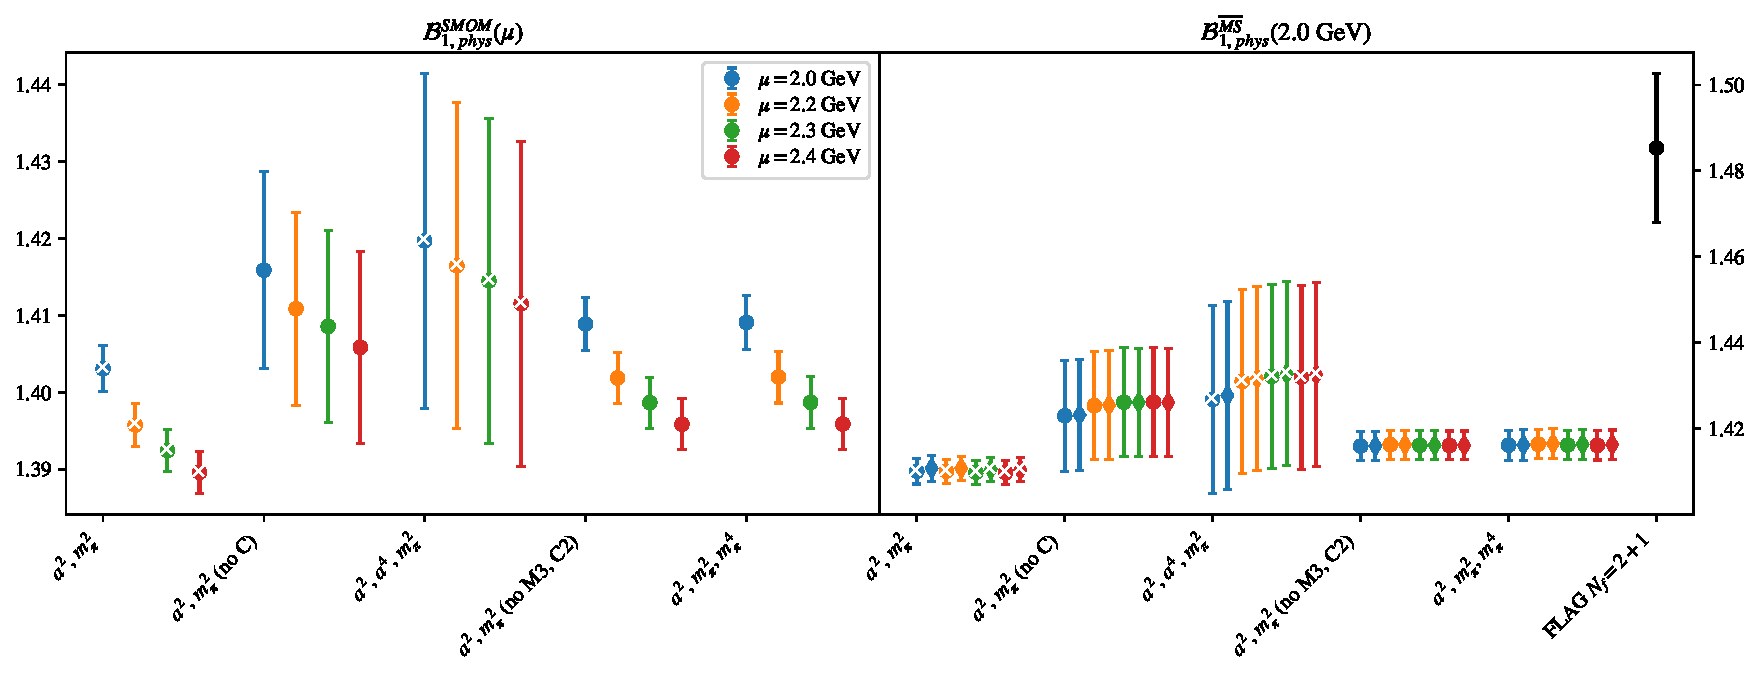
\includegraphics[page=1, width=1.1\textwidth]{VVpAA/SUSY/fit_summary.pdf}
\caption{$B_{1}$\\(left) $B_{phys}$ in RI/SMOM scheme from fit variations (fits with $p$-value $<0.05$ marked with ``$\times$"). \\(right) $B_{phys}$ in $\overline{MS}$ computed using $B^{\overline{MS}} = R^{\overline{MS}\leftarrow SMOM}(2.0)\sigma_{npt}(2.0,\mu) B^{SMOM}(\mu)$.}
\end{figure}
\clearpage
\begin{figure}
\centering
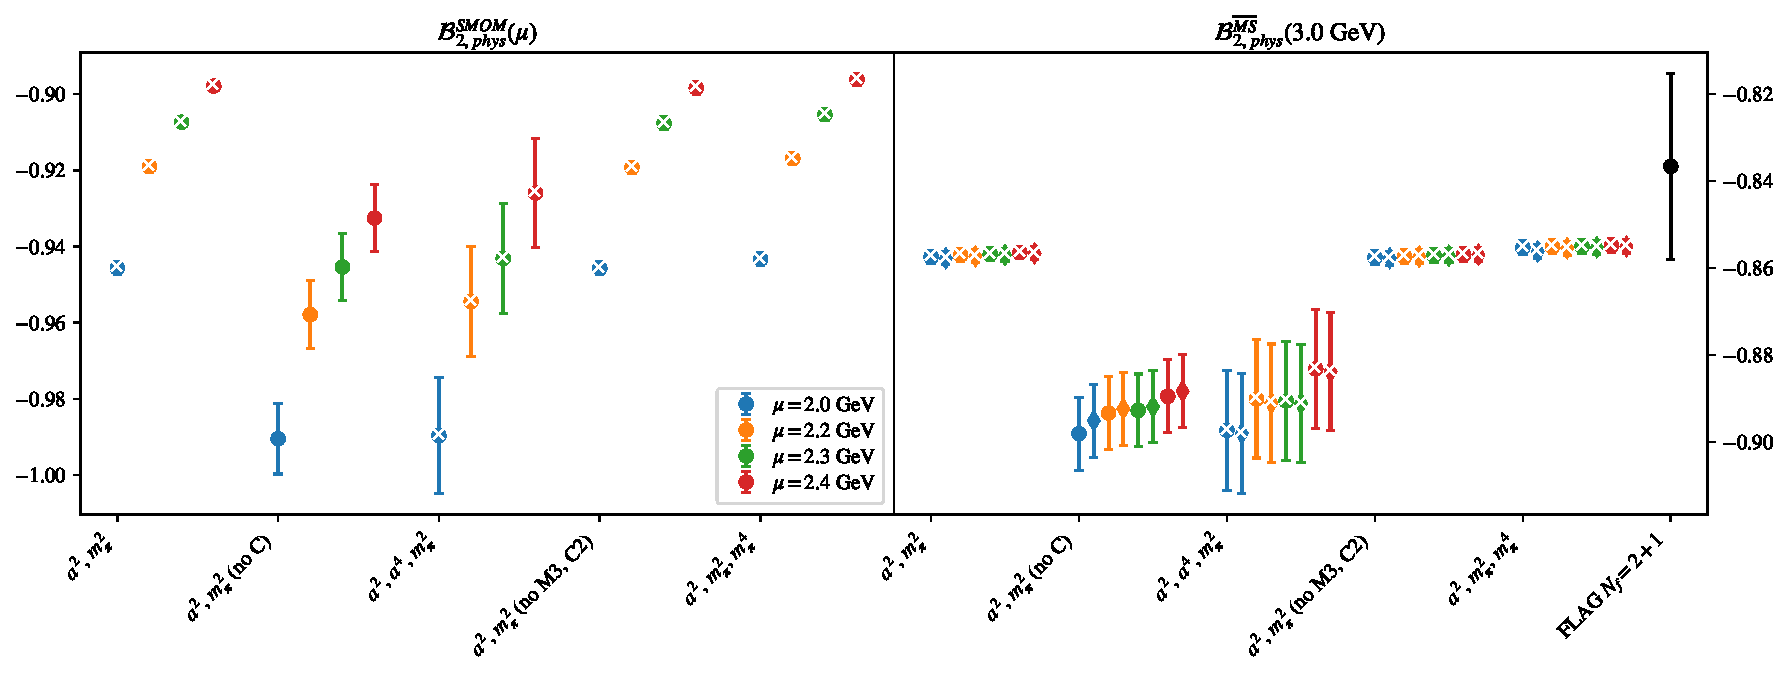
\includegraphics[page=1, width=1.1\textwidth]{VVmAA/SUSY/fit_summary.pdf}
\caption{$B_{2}$\\(left) $B_{phys}$ in RI/SMOM scheme from fit variations (fits with $p$-value $<0.05$ marked with ``$\times$"). \\(right) $B_{phys}$ in $\overline{MS}$ computed using $B^{\overline{MS}} = R^{\overline{MS}\leftarrow SMOM}(3.0)\sigma_{npt}(3.0,\mu) B^{SMOM}(\mu)$.}
\end{figure}
\clearpage
\begin{figure}
\centering
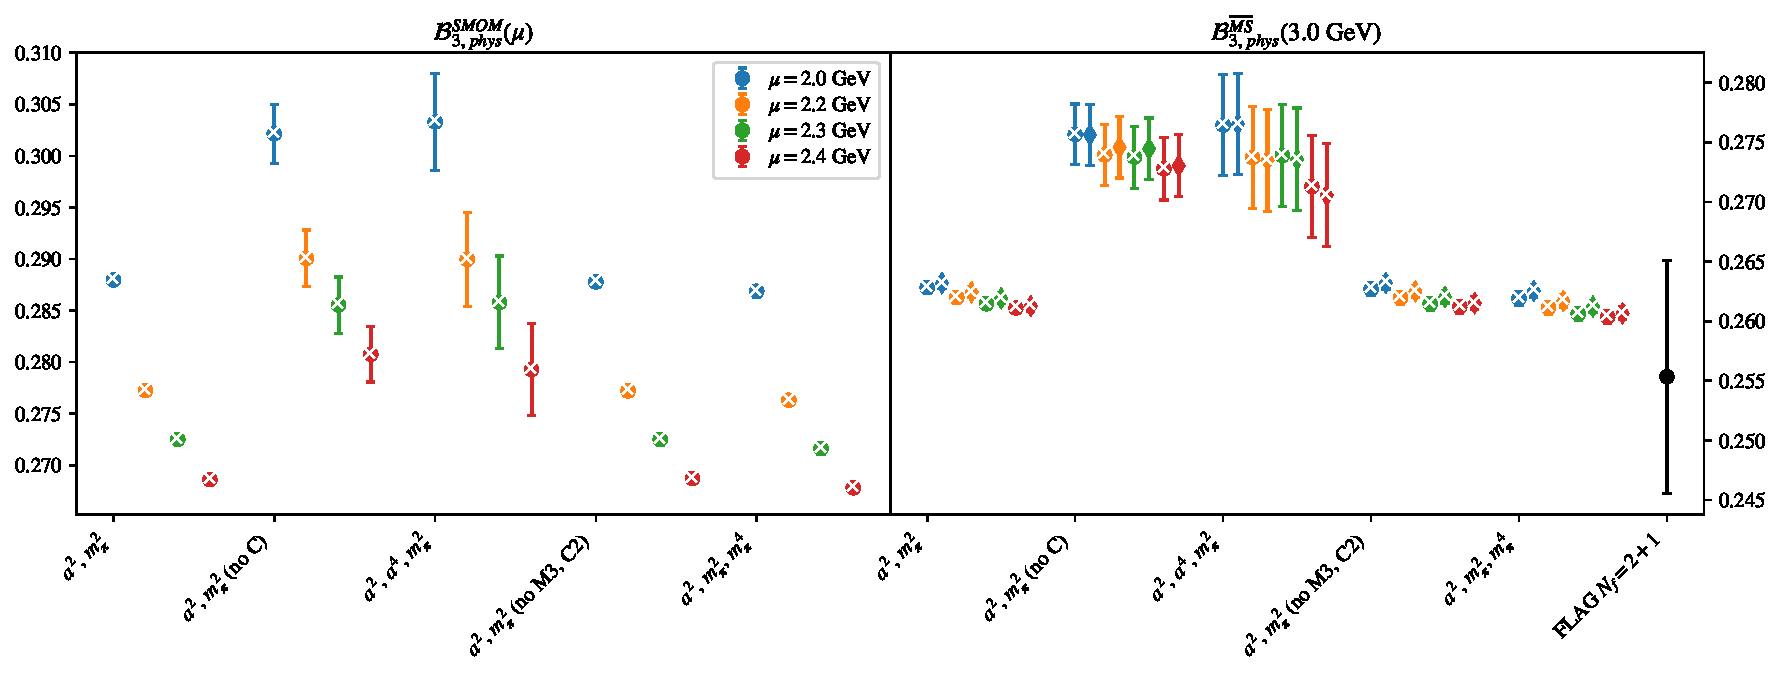
\includegraphics[page=1, width=1.1\textwidth]{SSmPP/SUSY/fit_summary.pdf}
\caption{$B_{3}$\\(left) $B_{phys}$ in RI/SMOM scheme from fit variations (fits with $p$-value $<0.05$ marked with ``$\times$"). \\(right) $B_{phys}$ in $\overline{MS}$ computed using $B^{\overline{MS}} = R^{\overline{MS}\leftarrow SMOM}(3.0)\sigma_{npt}(3.0,\mu) B^{SMOM}(\mu)$.}
\end{figure}
\clearpage
\begin{figure}
\centering
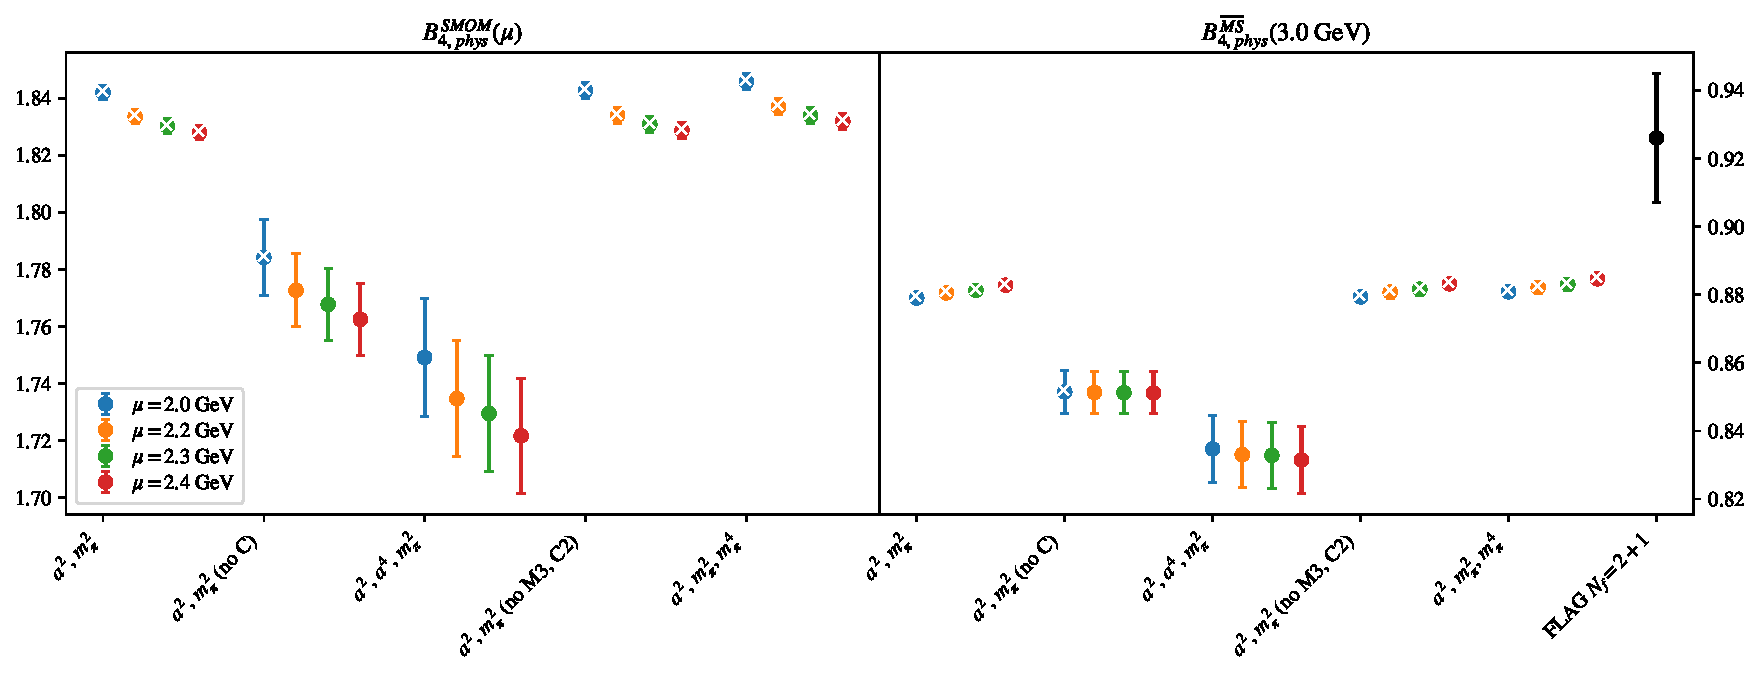
\includegraphics[page=1, width=1.1\textwidth]{SSpPP/SUSY/fit_summary.pdf}
\caption{$B_{4}$\\(left) $B_{phys}$ in RI/SMOM scheme from fit variations (fits with $p$-value $<0.05$ marked with ``$\times$"). \\(right) $B_{phys}$ in $\overline{MS}$ computed using $B^{\overline{MS}} = R^{\overline{MS}\leftarrow SMOM}(3.0)\sigma_{npt}(3.0,\mu) B^{SMOM}(\mu)$.}
\end{figure}
\clearpage
\begin{figure}
\centering
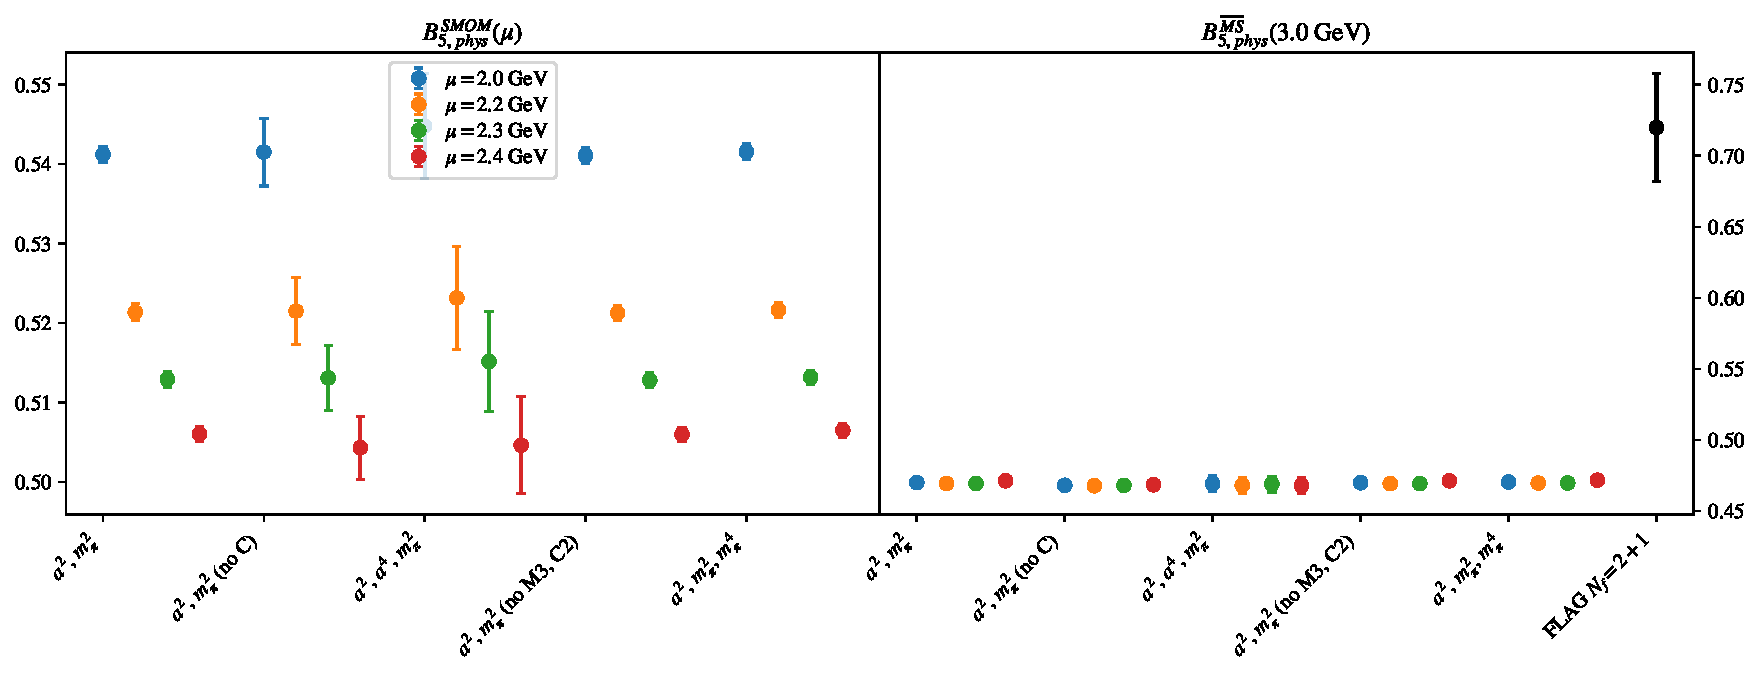
\includegraphics[page=1, width=1.1\textwidth]{TT/SUSY/fit_summary.pdf}
\caption{$B_{5}$\\(left) $B_{phys}$ in RI/SMOM scheme from fit variations (fits with $p$-value $<0.05$ marked with ``$\times$"). \\(right) $B_{phys}$ in $\overline{MS}$ computed using $B^{\overline{MS}} = R^{\overline{MS}\leftarrow SMOM}(3.0)\sigma_{npt}(3.0,\mu) B^{SMOM}(\mu)$.}
\end{figure}
\clearpage
\section{$B_1$}
\begin{table}[h!]
\begin{center}
\begin{tabular}{|c|c|c|c|c|c|}
\hline
$\mu$ (GeV) & $a^2$, $m_\pi^2$& $a^2$, $m_\pi^2$ (no C)& $a^2$, $a^4$, $m_\pi^2$& $a^2$, $m_\pi^2$ (no M3, C2)& $a^2$, $m_\pi^2$, $m_\pi^4$\\
\hline
2.0& \hyperlink{VVpAA/SUSY/a2m2_20.pdf.1}{\textbf{0.5264(10)}: 1.858 (0.098)} & \hyperlink{VVpAA/SUSY/a2m2noC_20.pdf.1}{\textbf{0.5310(47)}: 0.876 (0.417)} & \hyperlink{VVpAA/SUSY/a2a4m2_20.pdf.1}{\textbf{0.5327(81)}: 2.173 (0.069)} & \hyperlink{VVpAA/SUSY/a2m2mcut_20.pdf.1}{\textbf{0.5283(12)}: 0.248 (0.863)} & \hyperlink{VVpAA/SUSY/a2m2m4_20.pdf.1}{\textbf{0.5284(12)}: 0.661 (0.619)}\\
2.2& \hyperlink{VVpAA/SUSY/a2m2_22.pdf.1}{\textbf{0.5236(10)}: 2.214 (0.05)} & \hyperlink{VVpAA/SUSY/a2m2noC_22.pdf.1}{\textbf{0.5291(46)}: 1.143 (0.319)} & \hyperlink{VVpAA/SUSY/a2a4m2_22.pdf.1}{\textbf{0.5314(79)}: 2.525 (0.039)} & \hyperlink{VVpAA/SUSY/a2m2mcut_22.pdf.1}{\textbf{0.5257(12)}: 0.36 (0.782)} & \hyperlink{VVpAA/SUSY/a2m2m4_22.pdf.1}{\textbf{0.5257(12)}: 0.923 (0.449)}\\
2.3& \hyperlink{VVpAA/SUSY/a2m2_23.pdf.1}{\textbf{0.5224(10)}: 2.304 (0.042)} & \hyperlink{VVpAA/SUSY/a2m2noC_23.pdf.1}{\textbf{0.5282(46)}: 1.197 (0.302)} & \hyperlink{VVpAA/SUSY/a2a4m2_23.pdf.1}{\textbf{0.5306(78)}: 2.605 (0.034)} & \hyperlink{VVpAA/SUSY/a2m2mcut_23.pdf.1}{\textbf{0.5245(12)}: 0.411 (0.745)} & \hyperlink{VVpAA/SUSY/a2m2m4_23.pdf.1}{\textbf{0.5245(12)}: 0.993 (0.41)}\\
2.4& \hyperlink{VVpAA/SUSY/a2m2_24.pdf.1}{\textbf{0.5213(10)}: 2.348 (0.039)} & \hyperlink{VVpAA/SUSY/a2m2noC_24.pdf.1}{\textbf{0.5271(46)}: 1.223 (0.294)} & \hyperlink{VVpAA/SUSY/a2a4m2_24.pdf.1}{\textbf{0.5295(78)}: 2.663 (0.031)} & \hyperlink{VVpAA/SUSY/a2m2mcut_24.pdf.1}{\textbf{0.5234(12)}: 0.411 (0.745)} & \hyperlink{VVpAA/SUSY/a2m2m4_24.pdf.1}{\textbf{0.5235(12)}: 1.005 (0.403)}\\
\hline
\end{tabular}
\caption{Physical point value from chiral and continuum extrapolation at renormalisation scale $\mu$. Entries are \textbf{value(error)}: $\chi^2/\text{DOF}$ ($p$-value).}
\end{center}
\end{table}
\begin{table}[h!]
\begin{center}
\begin{tabular}{|c c|c|c|c|c|c|}
\hline
$\mu$ (GeV) &  & $a^2$, $m_\pi^2$& $a^2$, $m_\pi^2$ (no C)& $a^2$, $a^4$, $m_\pi^2$& $a^2$, $m_\pi^2$ (no M3, C2)& $a^2$, $m_\pi^2$, $m_\pi^4$\\
\hline
\multirow{2}{0.5in}{2.0} & $\alpha$ & 0.0937(71)& 0.047(53)& -0.017& 0.0815(83)& 0.0813(82)\\
 & $\beta$ & 0.00261(14)& 0.00223(27)& 0.00263(15)& 0.00189(28)& 0.00031(90)\\
\hline
\multirow{2}{0.5in}{2.2} & $\alpha$ & 0.0977(70)& 0.041(52)& -0.038& 0.0847(83)& 0.0846(82)\\
 & $\beta$ & 0.00261(14)& 0.00220(27)& 0.00264(14)& 0.00184(28)& 0.00020(89)\\
\hline
\multirow{2}{0.5in}{2.3} & $\alpha$ & 0.0992(70)& 0.039(52)& -0.045& 0.0859(83)& 0.0859(82)\\
 & $\beta$ & 0.00262(14)& 0.00220(27)& 0.00265(14)& 0.00184(28)& 0.00018(89)\\
\hline
\multirow{2}{0.5in}{2.4} & $\alpha$ & 0.0999(70)& 0.040(52)& -0.044& 0.0864(83)& 0.0864(82)\\
 & $\beta$ & 0.00263(14)& 0.00220(27)& 0.00266(14)& 0.00184(28)& 0.00017(89)\\
\hline
\end{tabular}
\caption{Fit values of coefficients in $B = B_{phys} + \mathbf{\alpha} a^2 + \mathbf{\beta}\left(\frac{m_\pi^2}{f_\pi^2}-\frac{m_{\pi,PDG}^2}{f_\pi^2}\right) + \ldots$.}
\end{center}
\end{table}
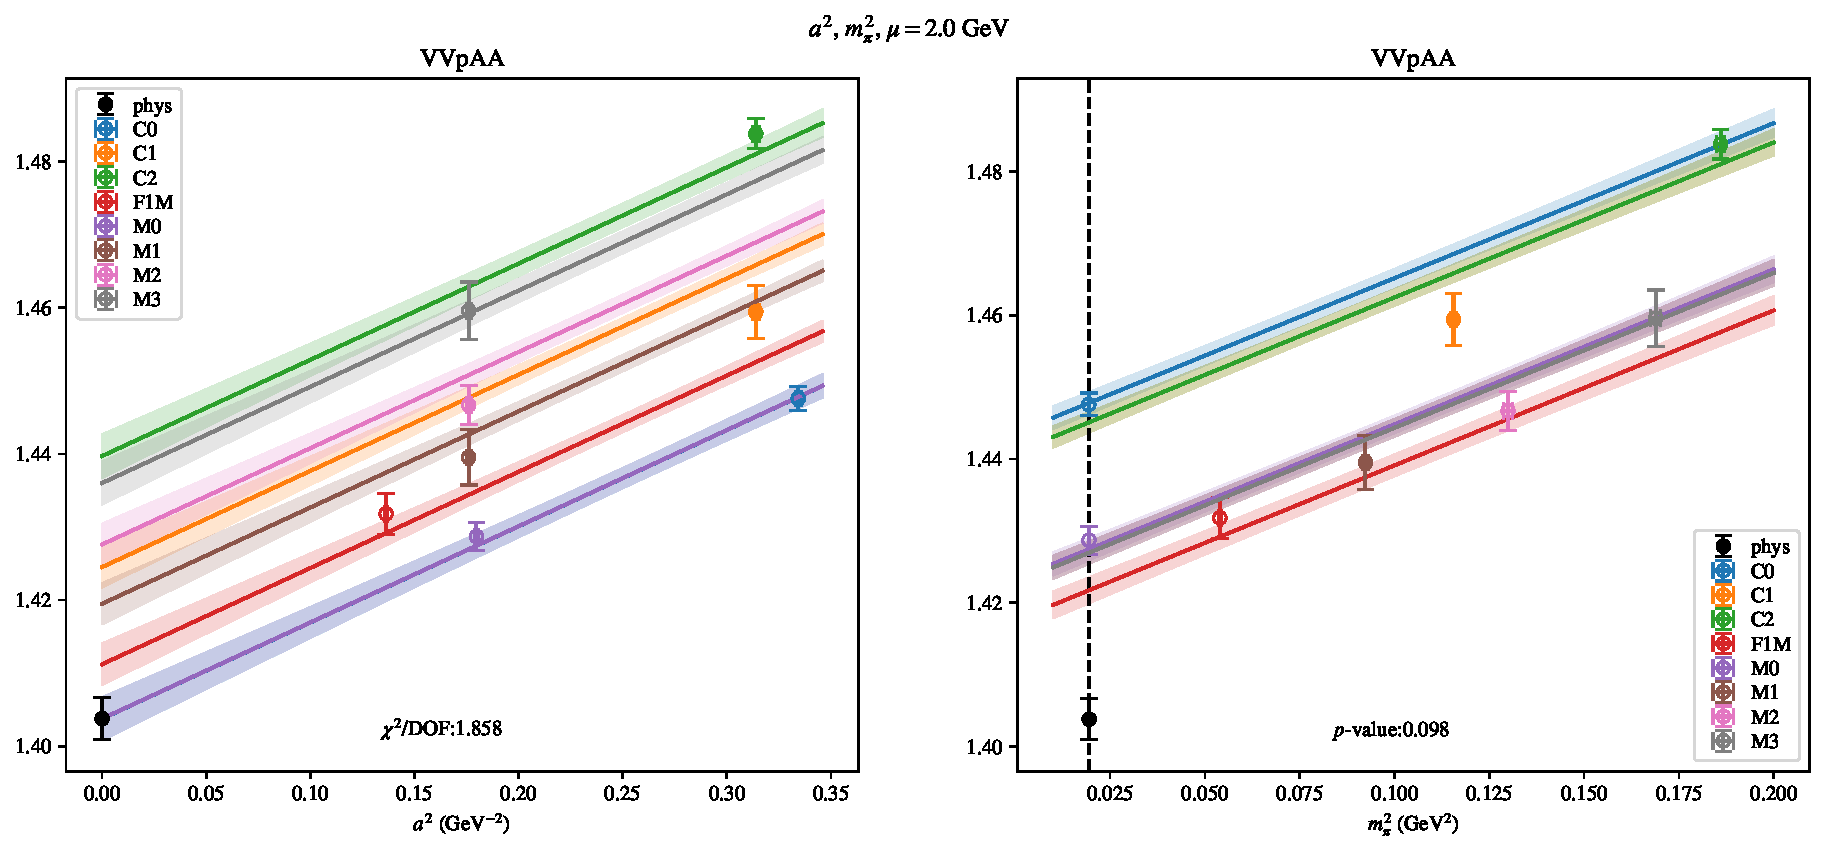
\includepdf[link, pages=-]{VVpAA/SUSY/a2m2_20.pdf}
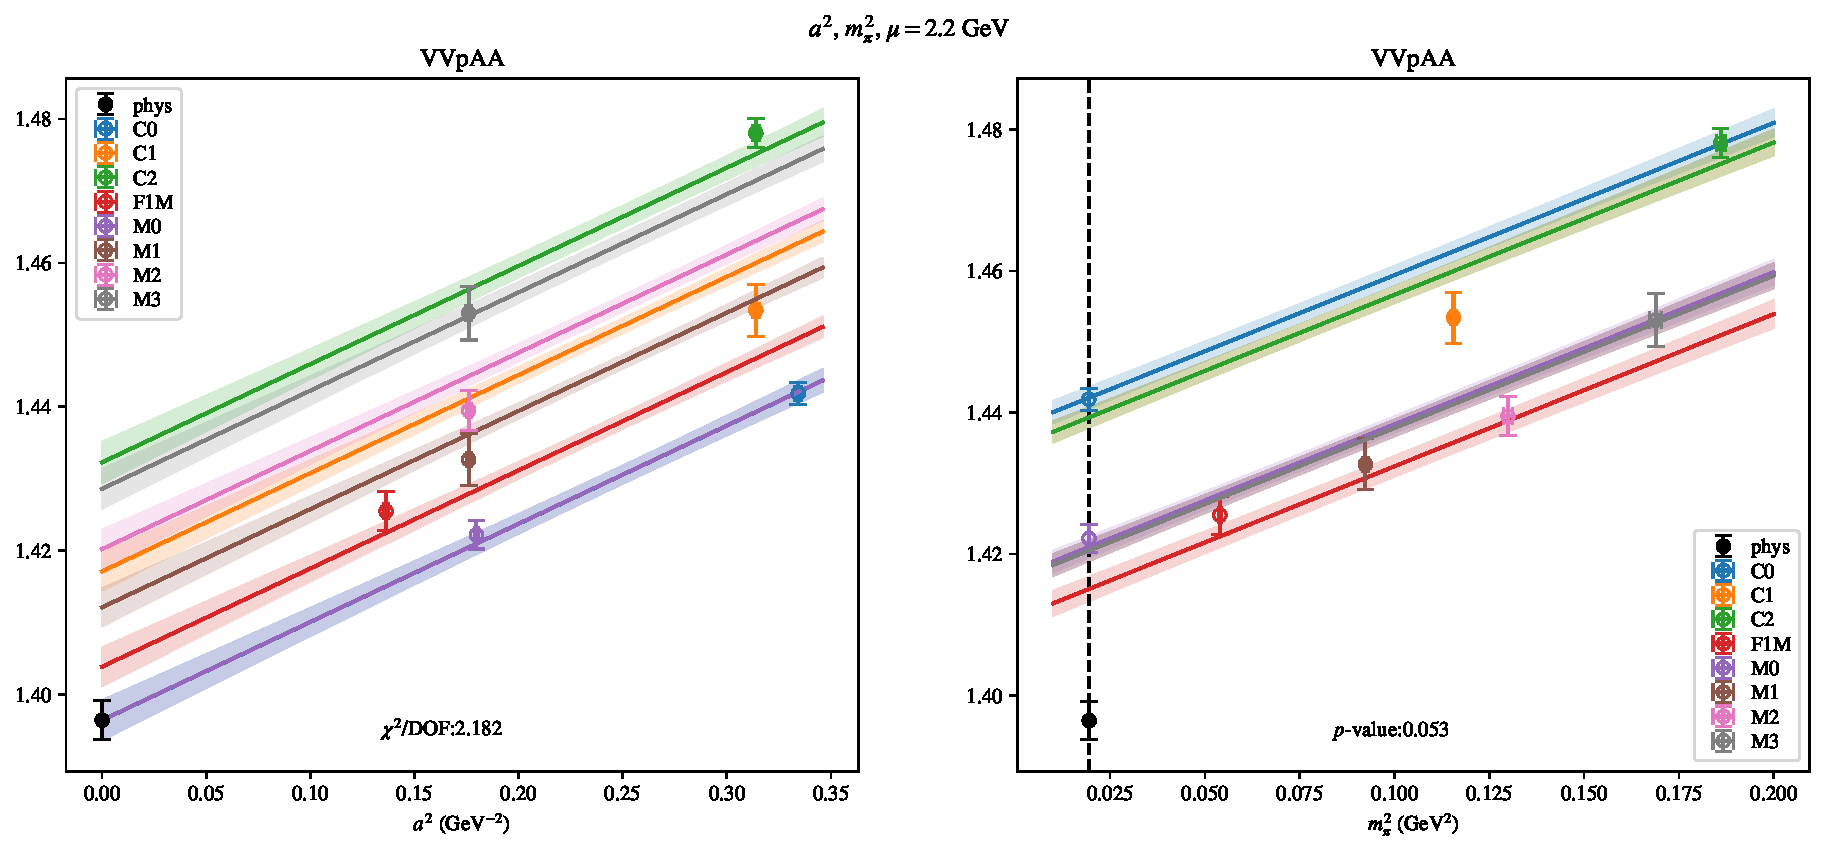
\includepdf[link, pages=-]{VVpAA/SUSY/a2m2_22.pdf}
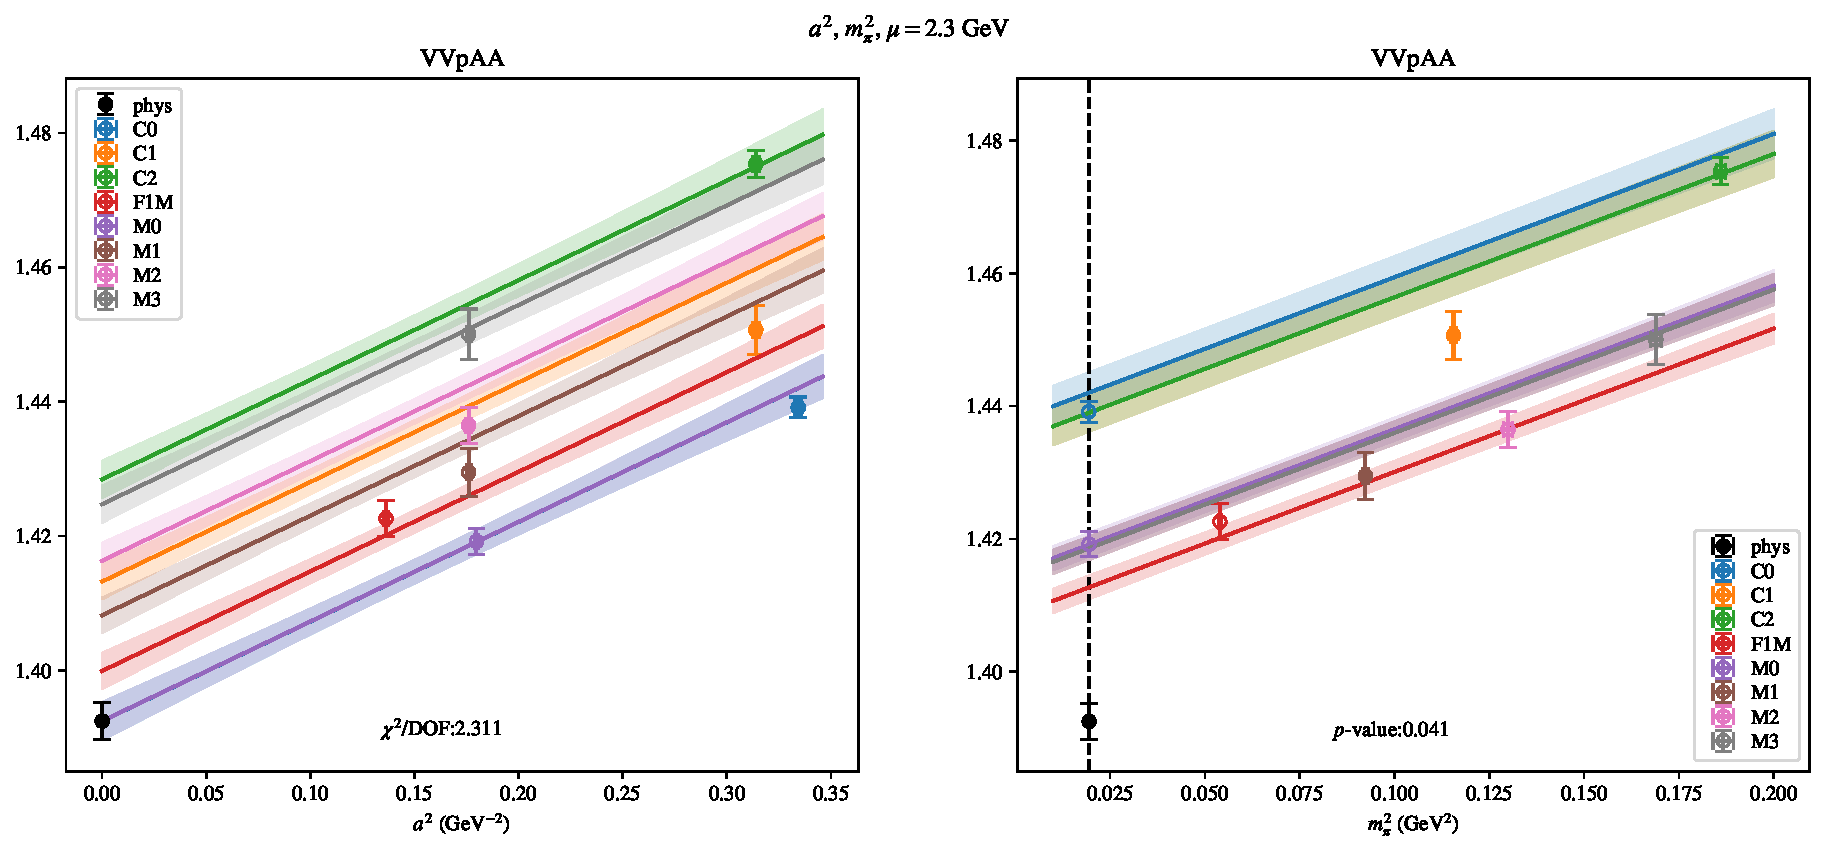
\includepdf[link, pages=-]{VVpAA/SUSY/a2m2_23.pdf}
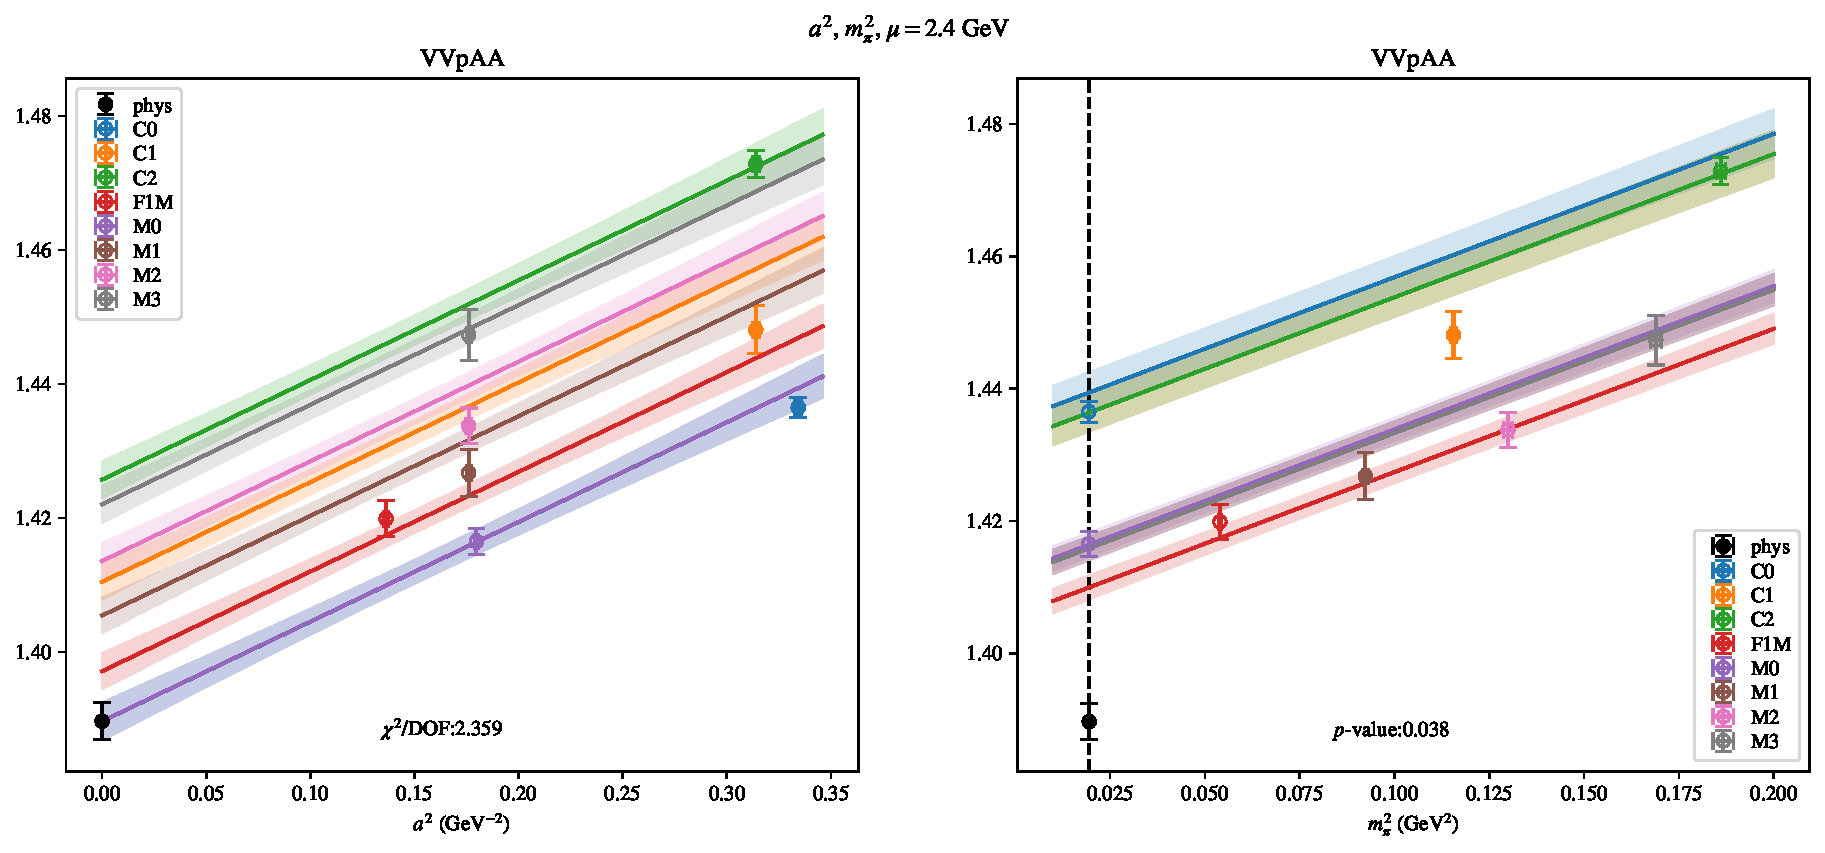
\includepdf[link, pages=-]{VVpAA/SUSY/a2m2_24.pdf}
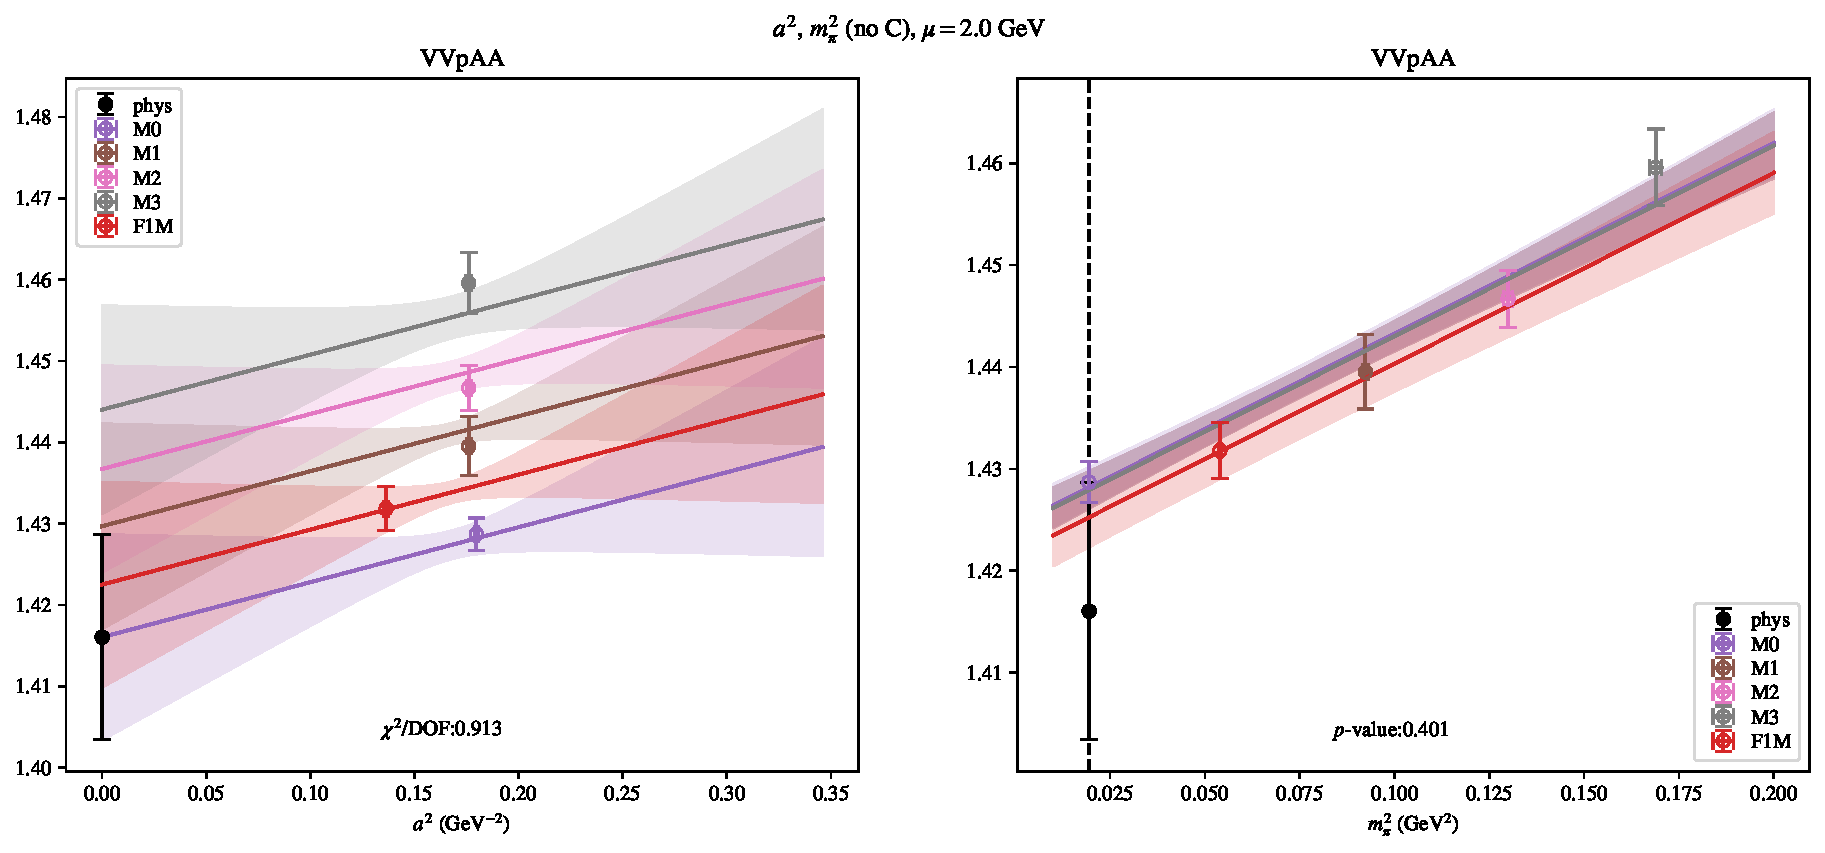
\includepdf[link, pages=-]{VVpAA/SUSY/a2m2noC_20.pdf}
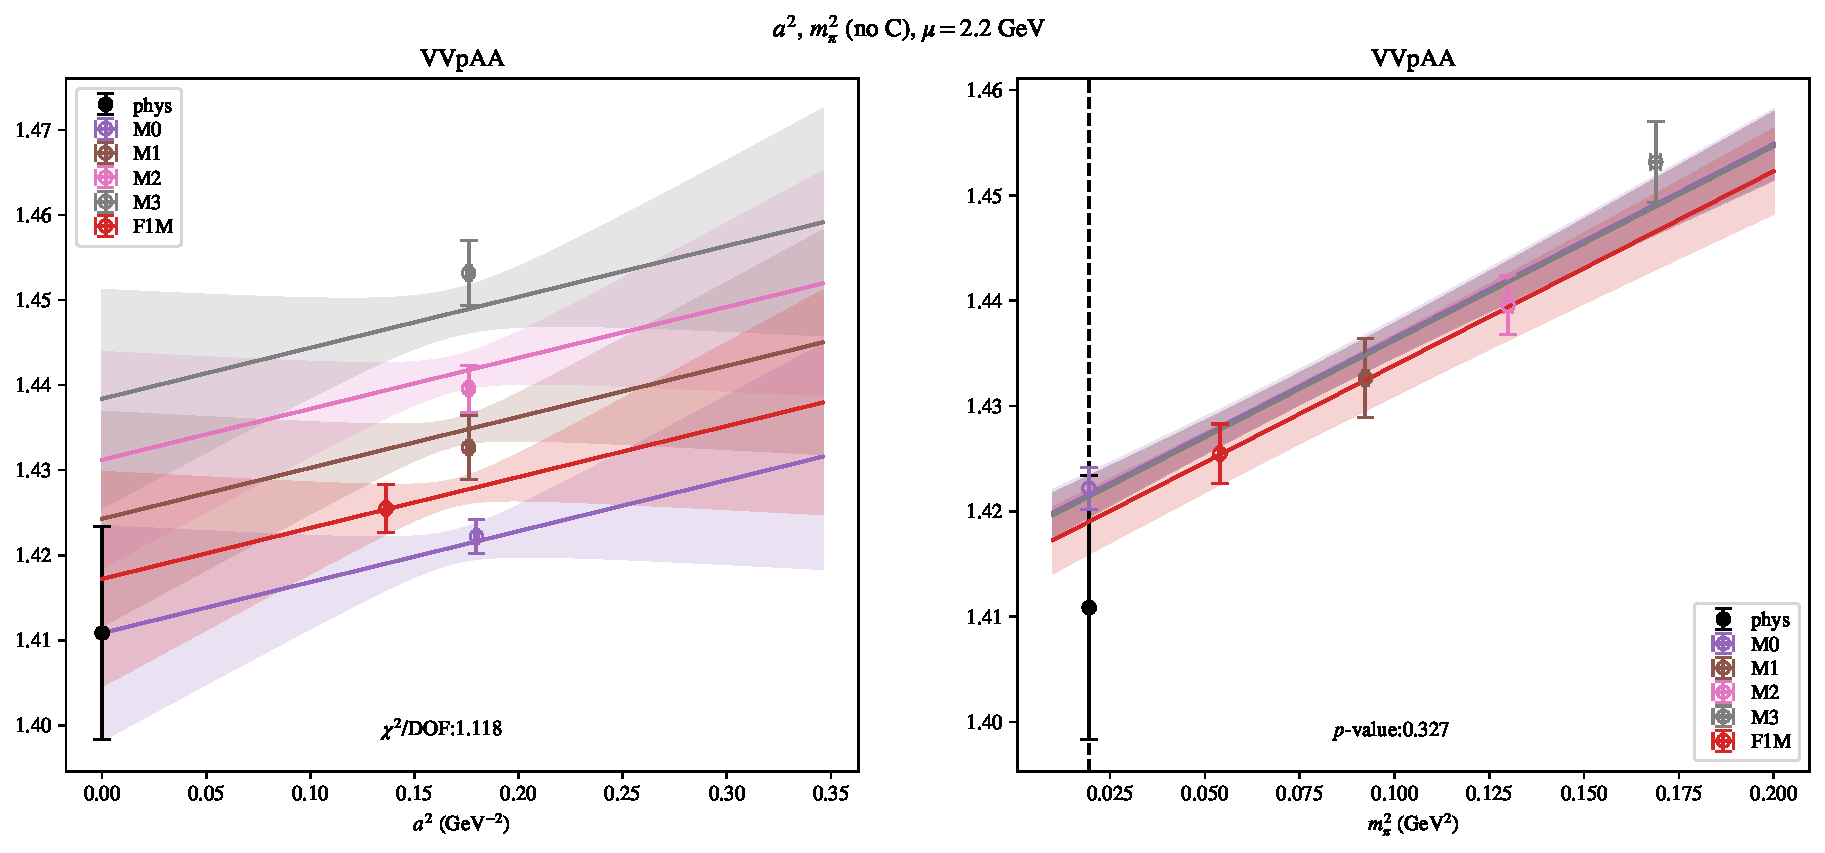
\includepdf[link, pages=-]{VVpAA/SUSY/a2m2noC_22.pdf}
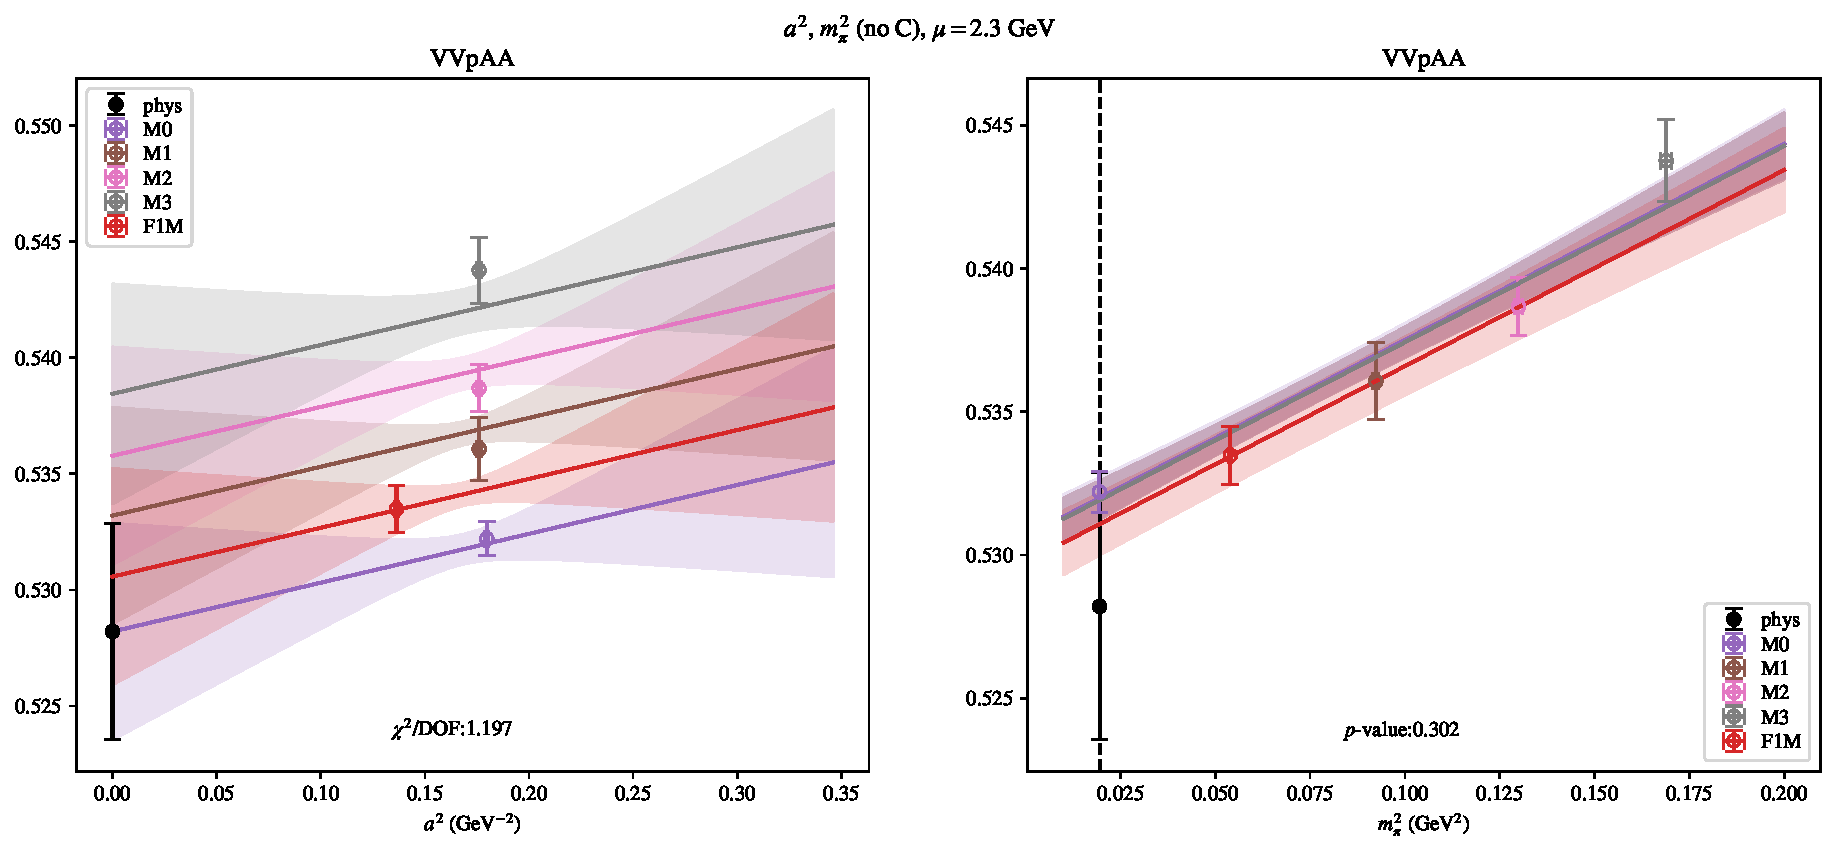
\includepdf[link, pages=-]{VVpAA/SUSY/a2m2noC_23.pdf}
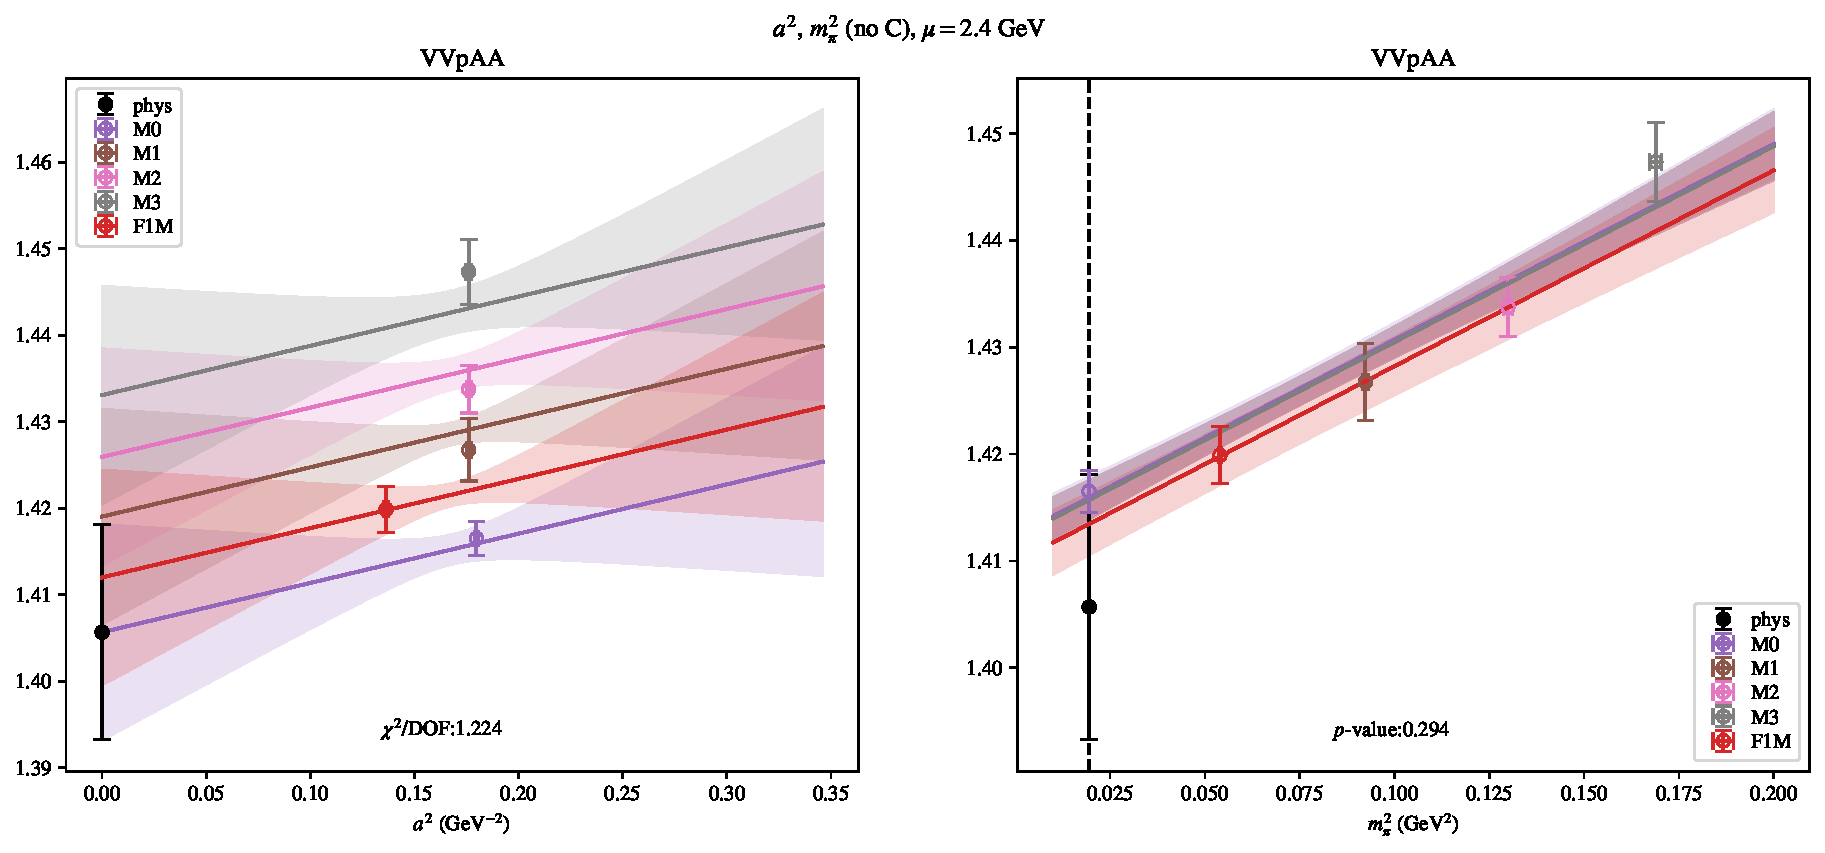
\includepdf[link, pages=-]{VVpAA/SUSY/a2m2noC_24.pdf}
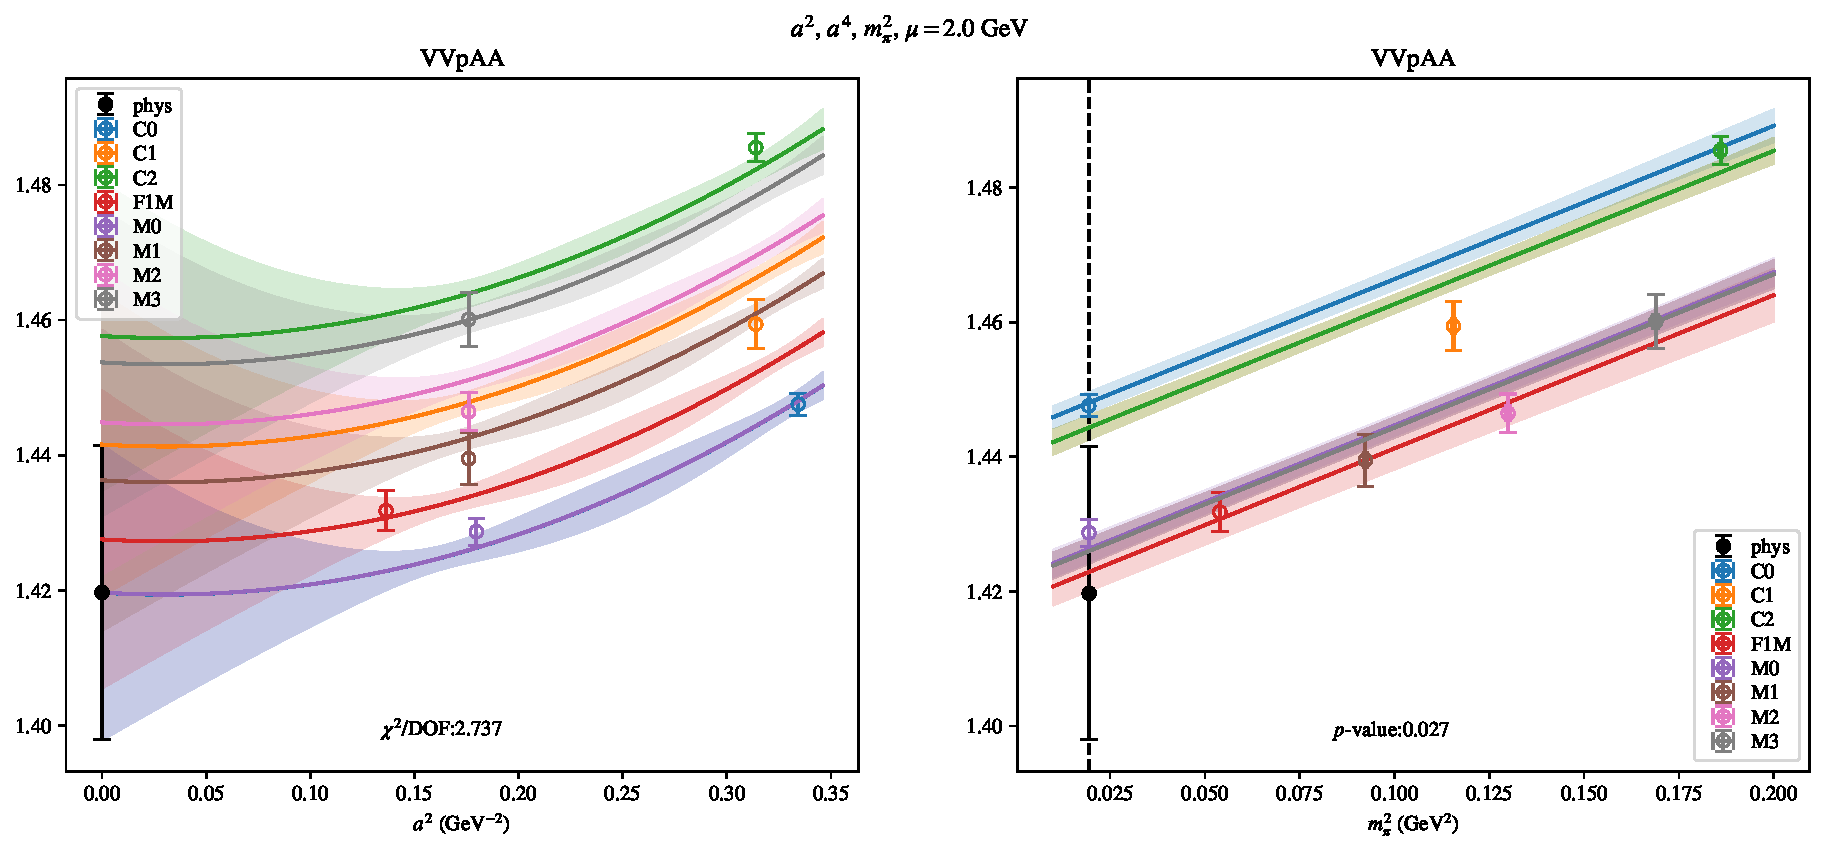
\includepdf[link, pages=-]{VVpAA/SUSY/a2a4m2_20.pdf}
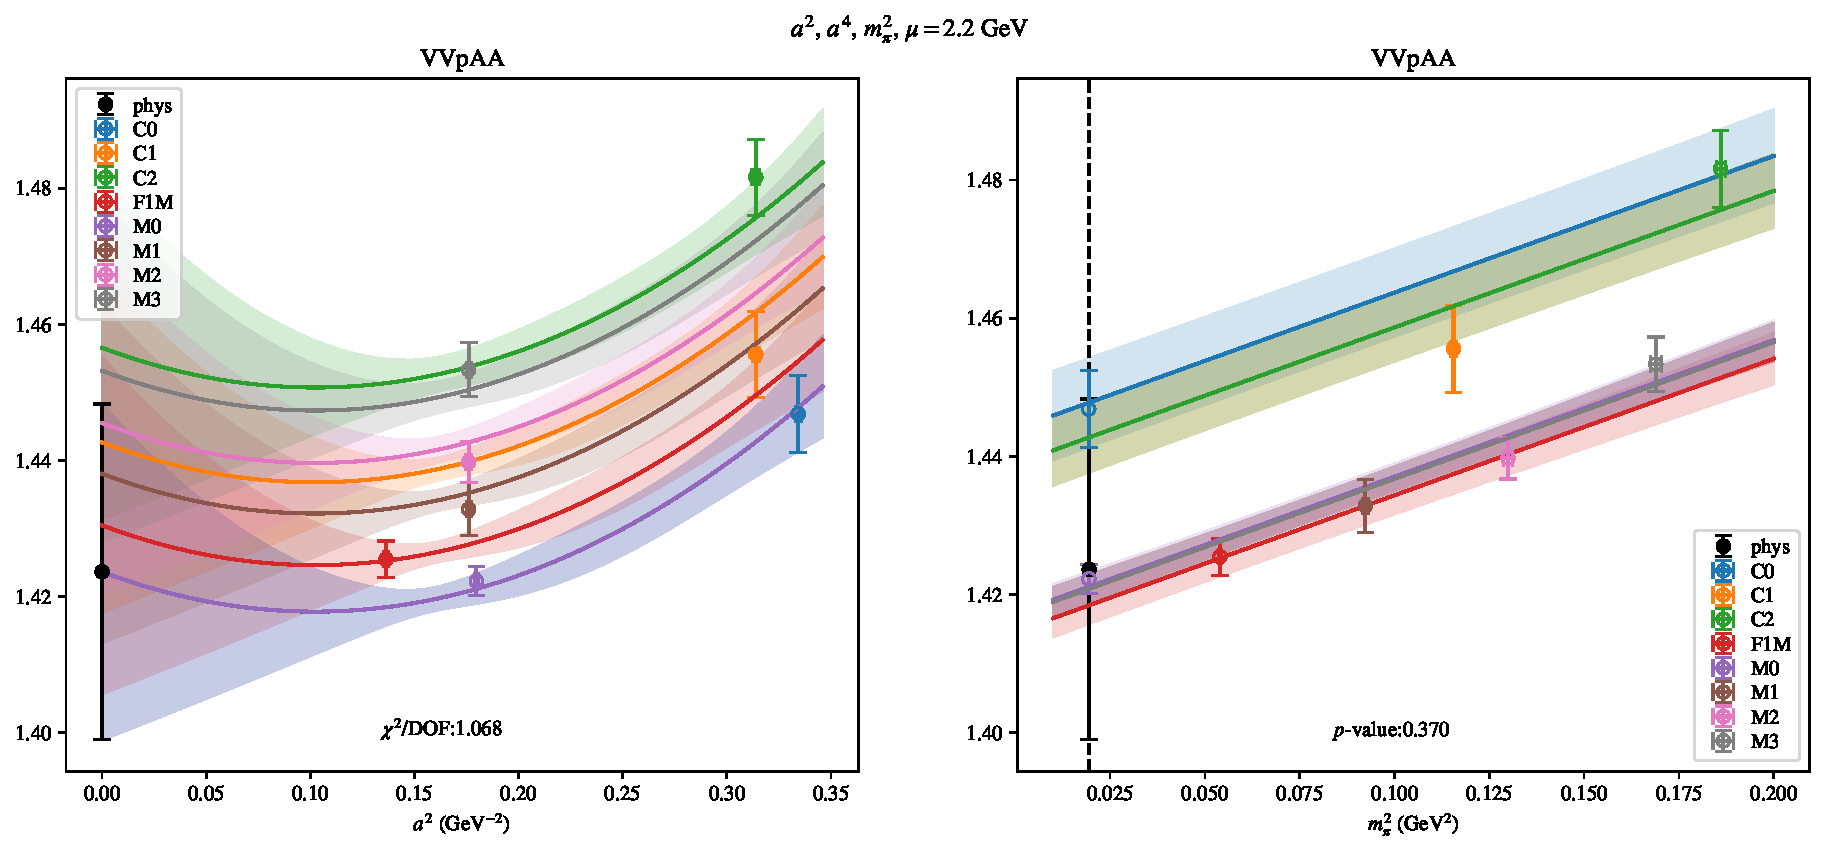
\includepdf[link, pages=-]{VVpAA/SUSY/a2a4m2_22.pdf}
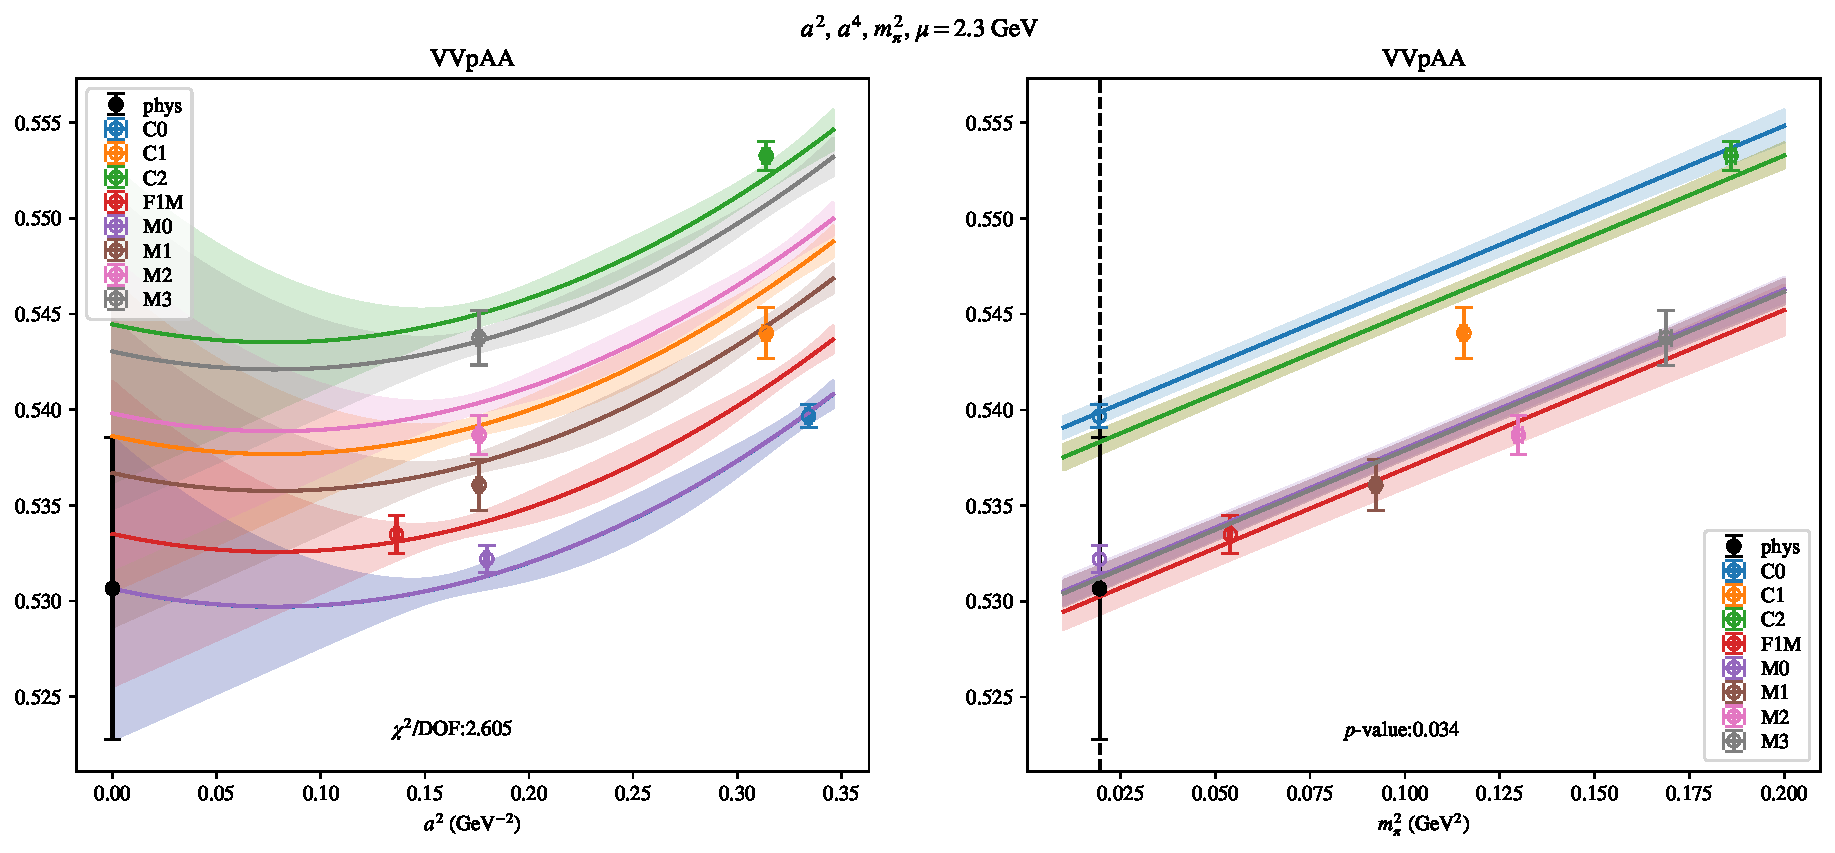
\includepdf[link, pages=-]{VVpAA/SUSY/a2a4m2_23.pdf}
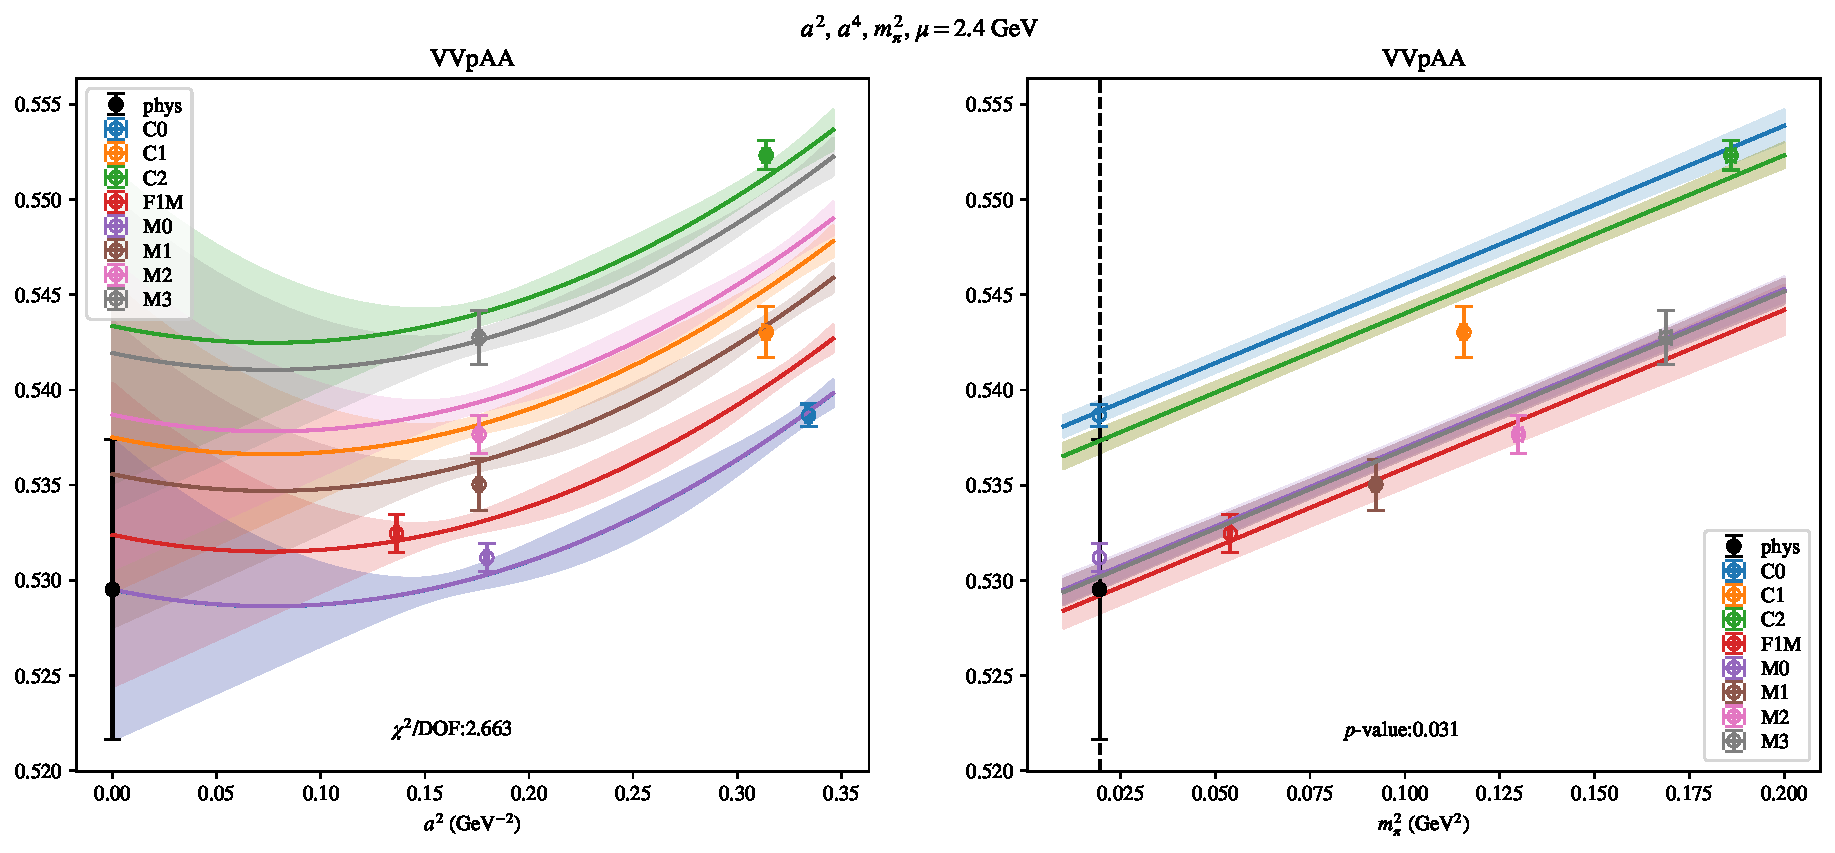
\includepdf[link, pages=-]{VVpAA/SUSY/a2a4m2_24.pdf}
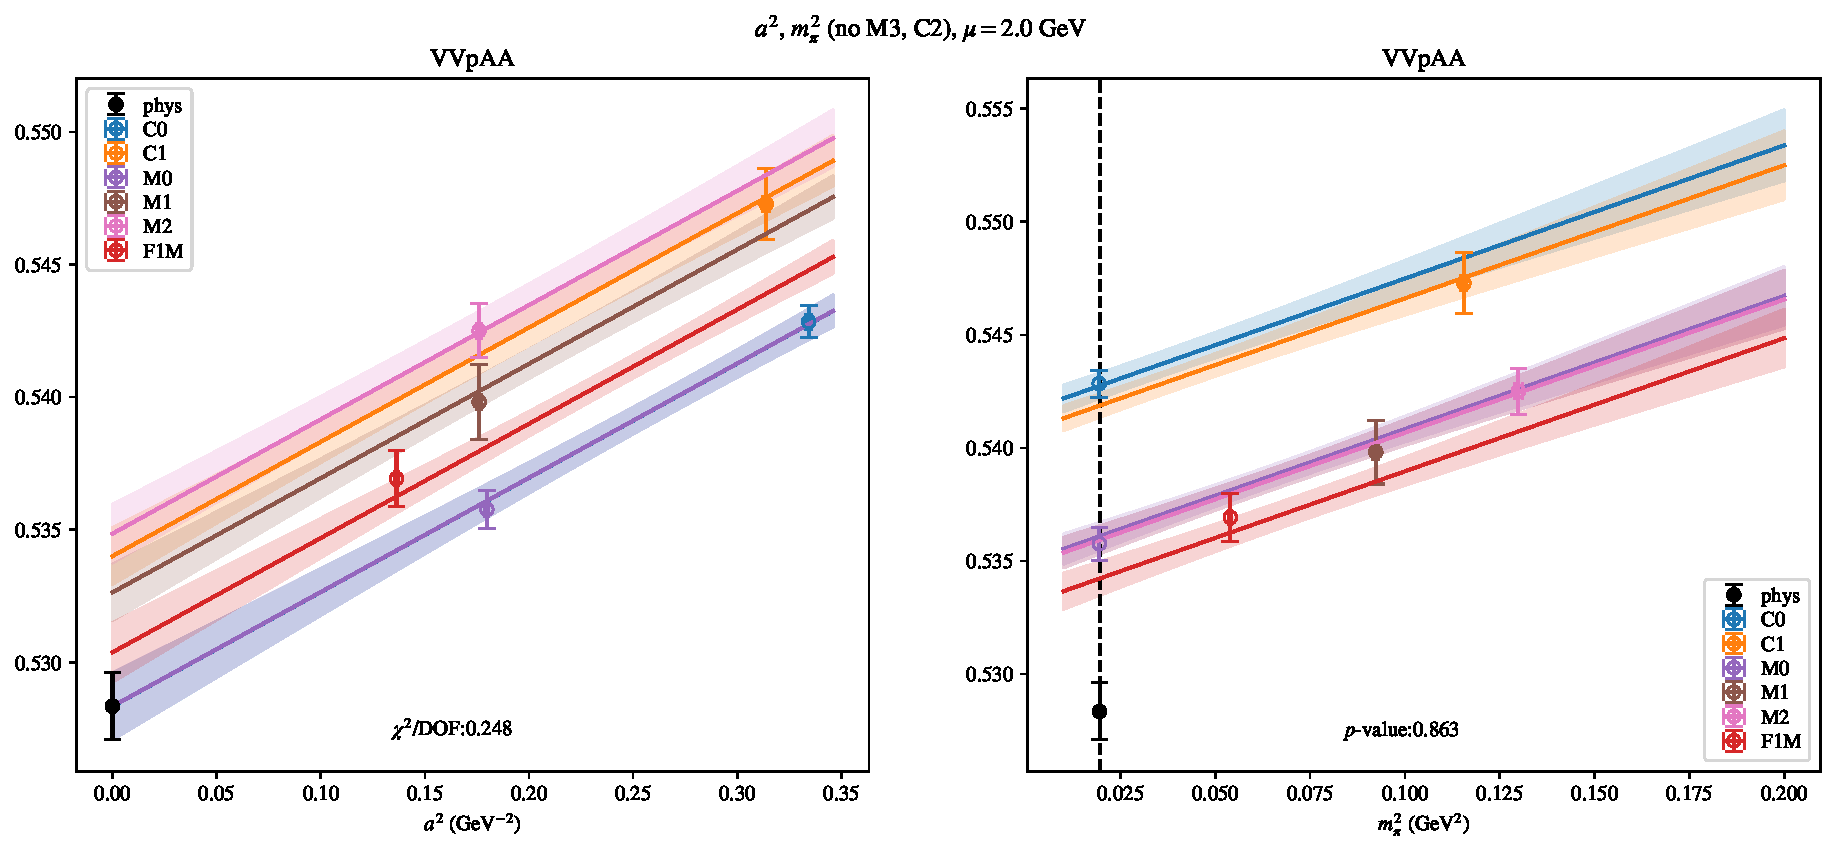
\includepdf[link, pages=-]{VVpAA/SUSY/a2m2mcut_20.pdf}
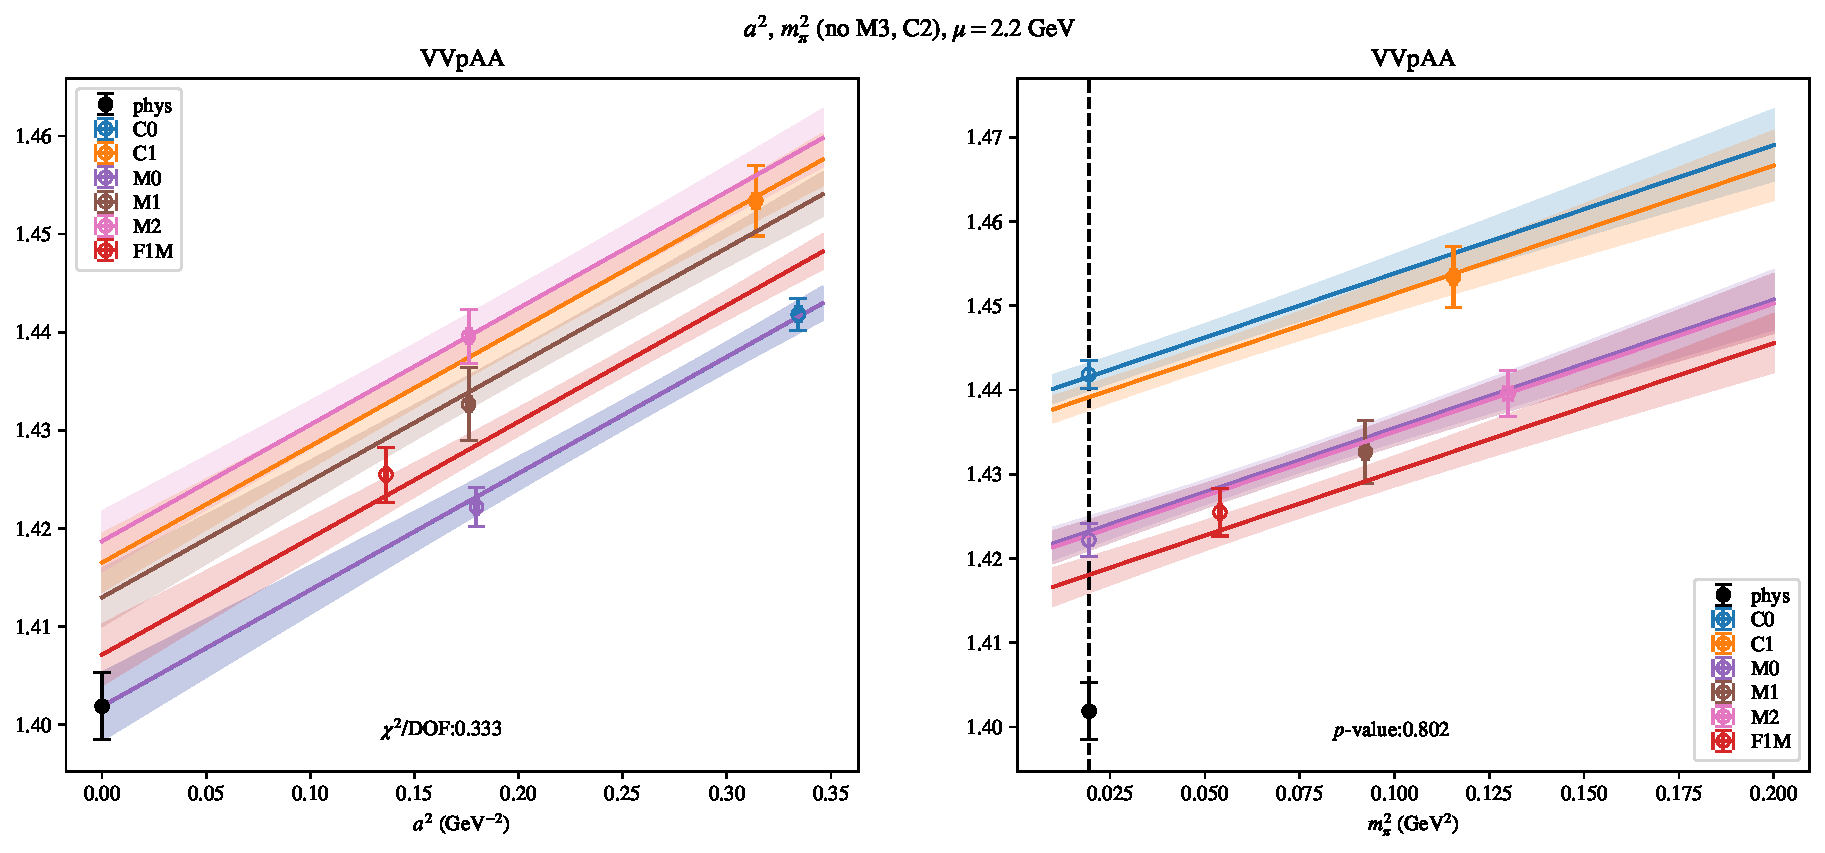
\includepdf[link, pages=-]{VVpAA/SUSY/a2m2mcut_22.pdf}
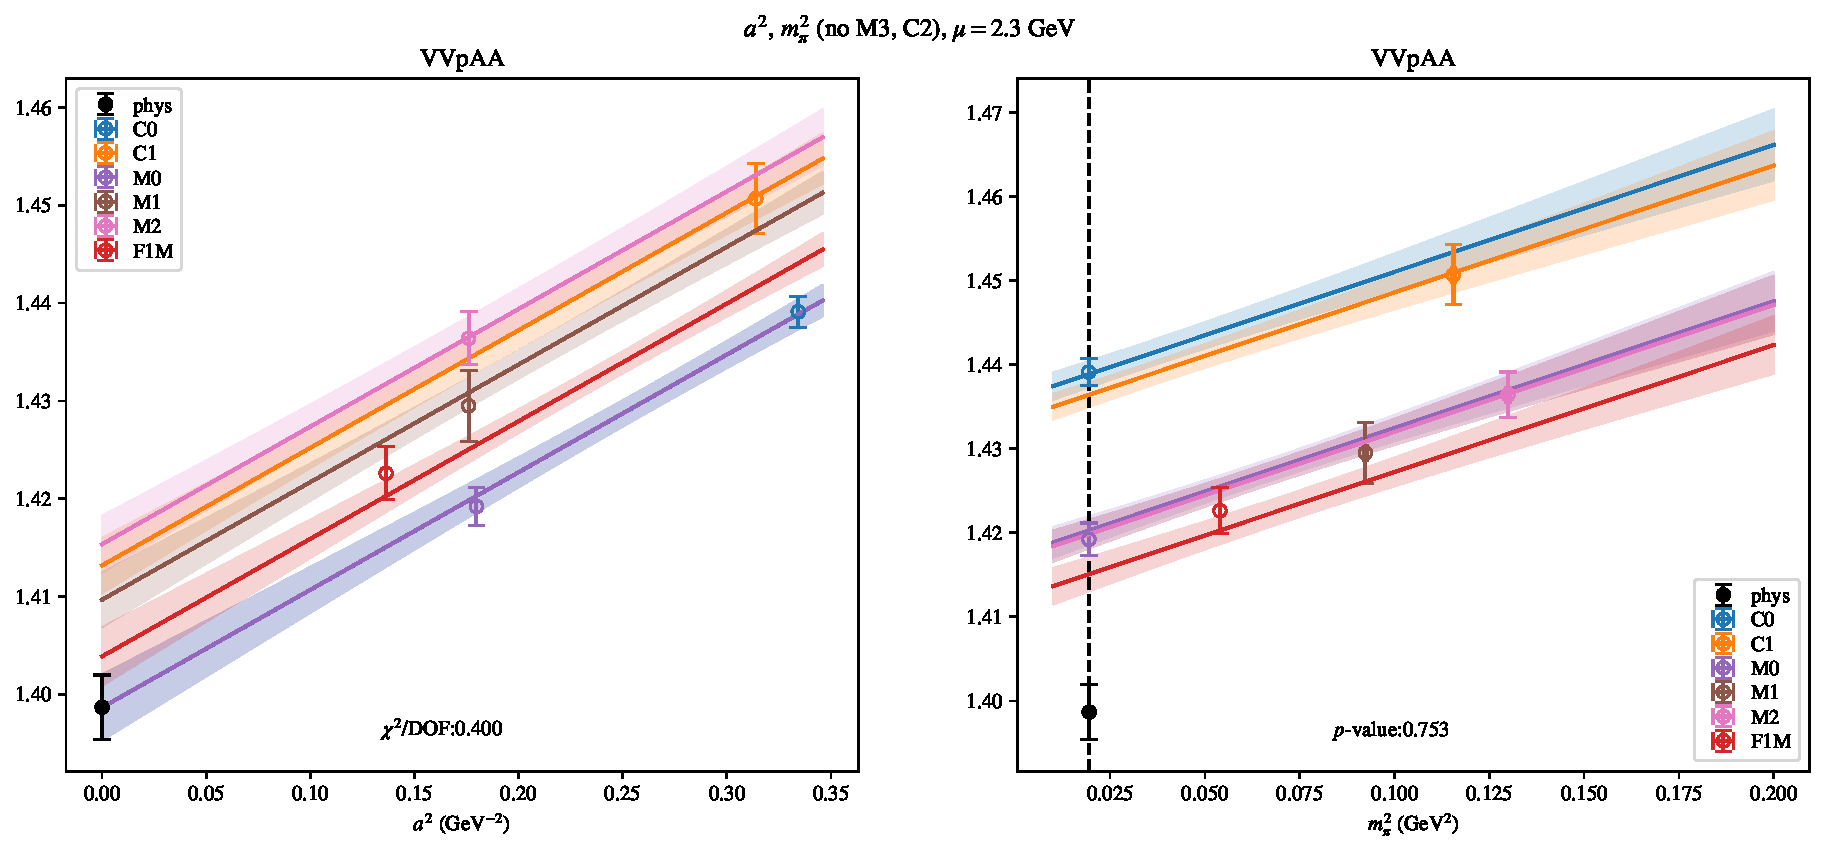
\includepdf[link, pages=-]{VVpAA/SUSY/a2m2mcut_23.pdf}
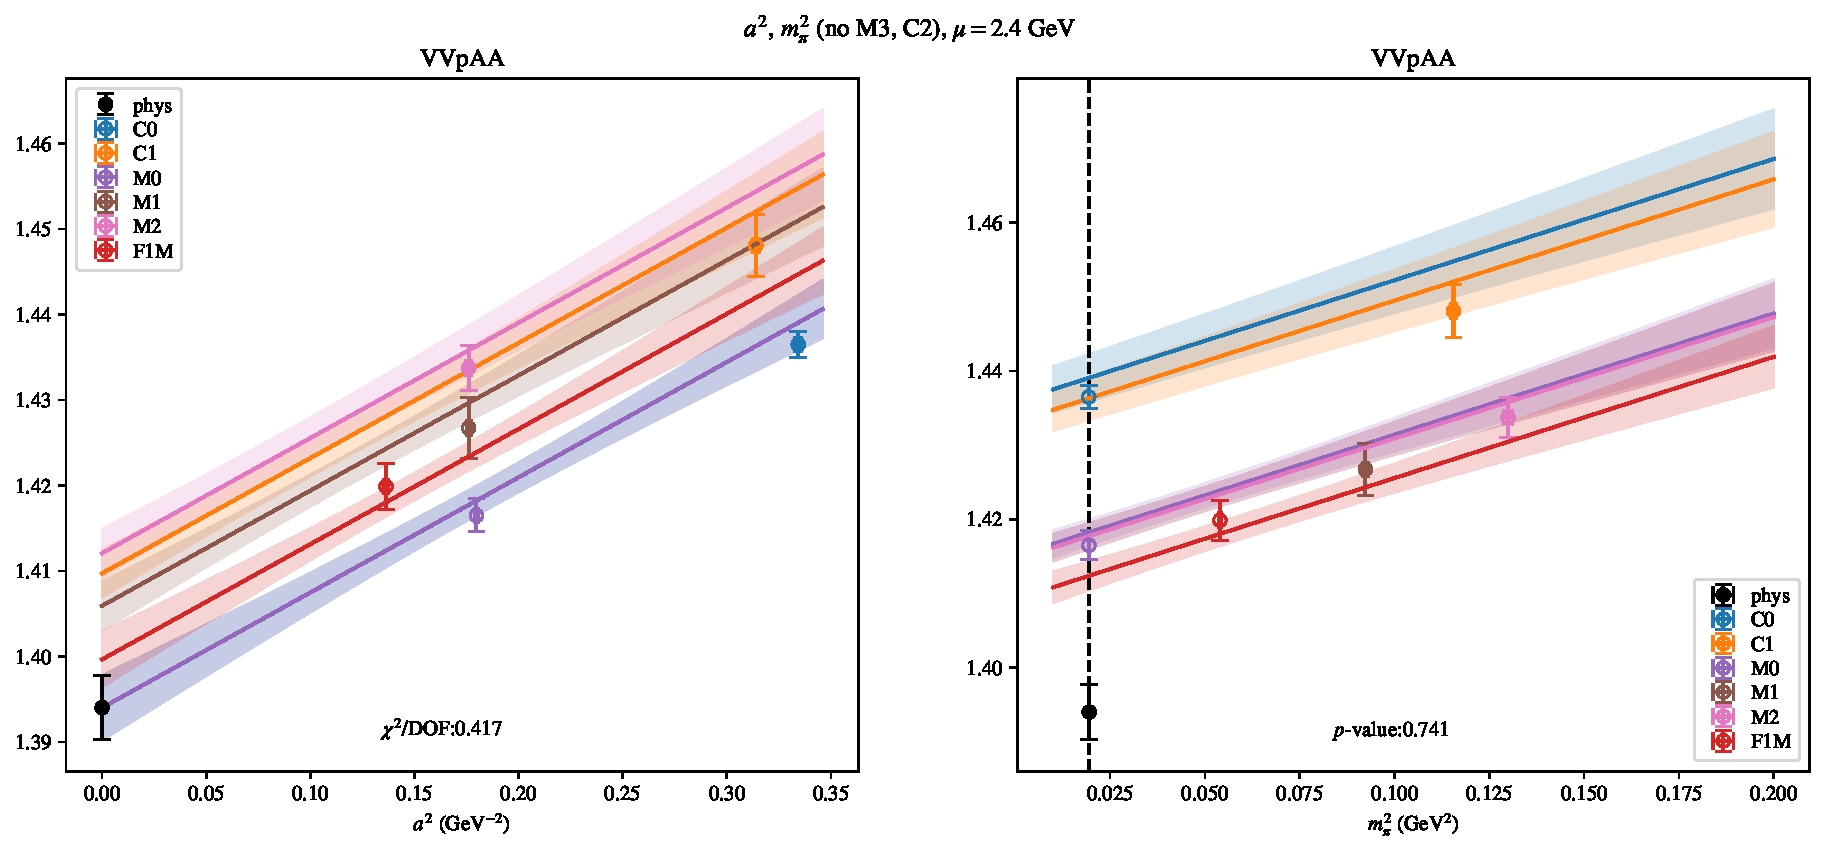
\includepdf[link, pages=-]{VVpAA/SUSY/a2m2mcut_24.pdf}
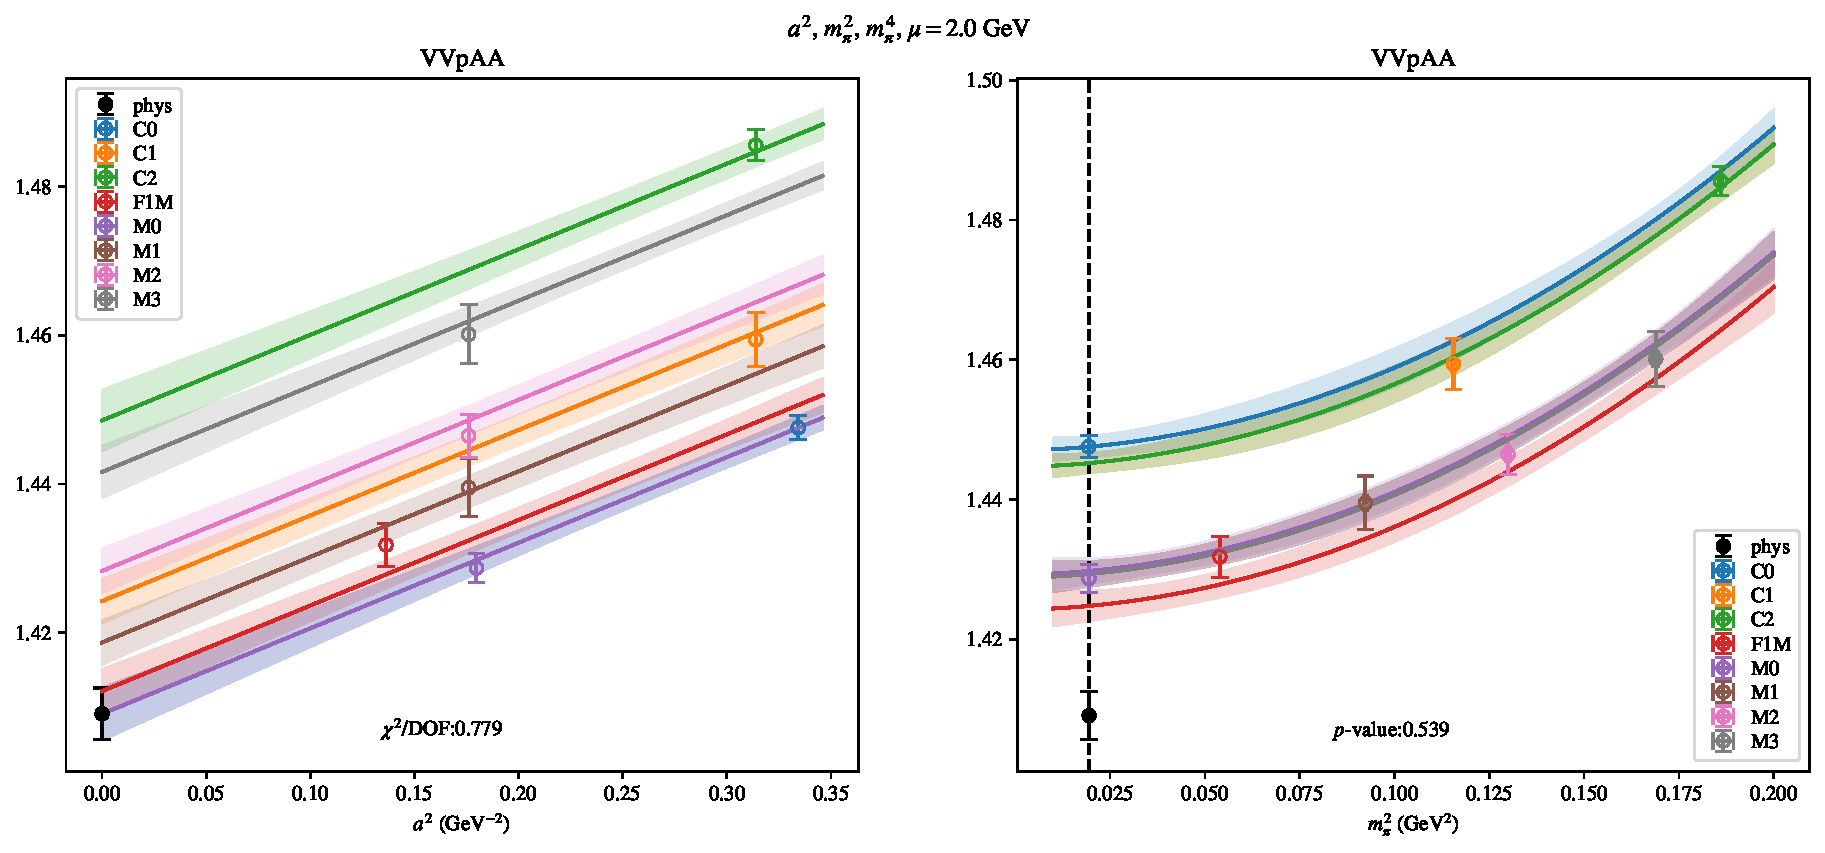
\includepdf[link, pages=-]{VVpAA/SUSY/a2m2m4_20.pdf}
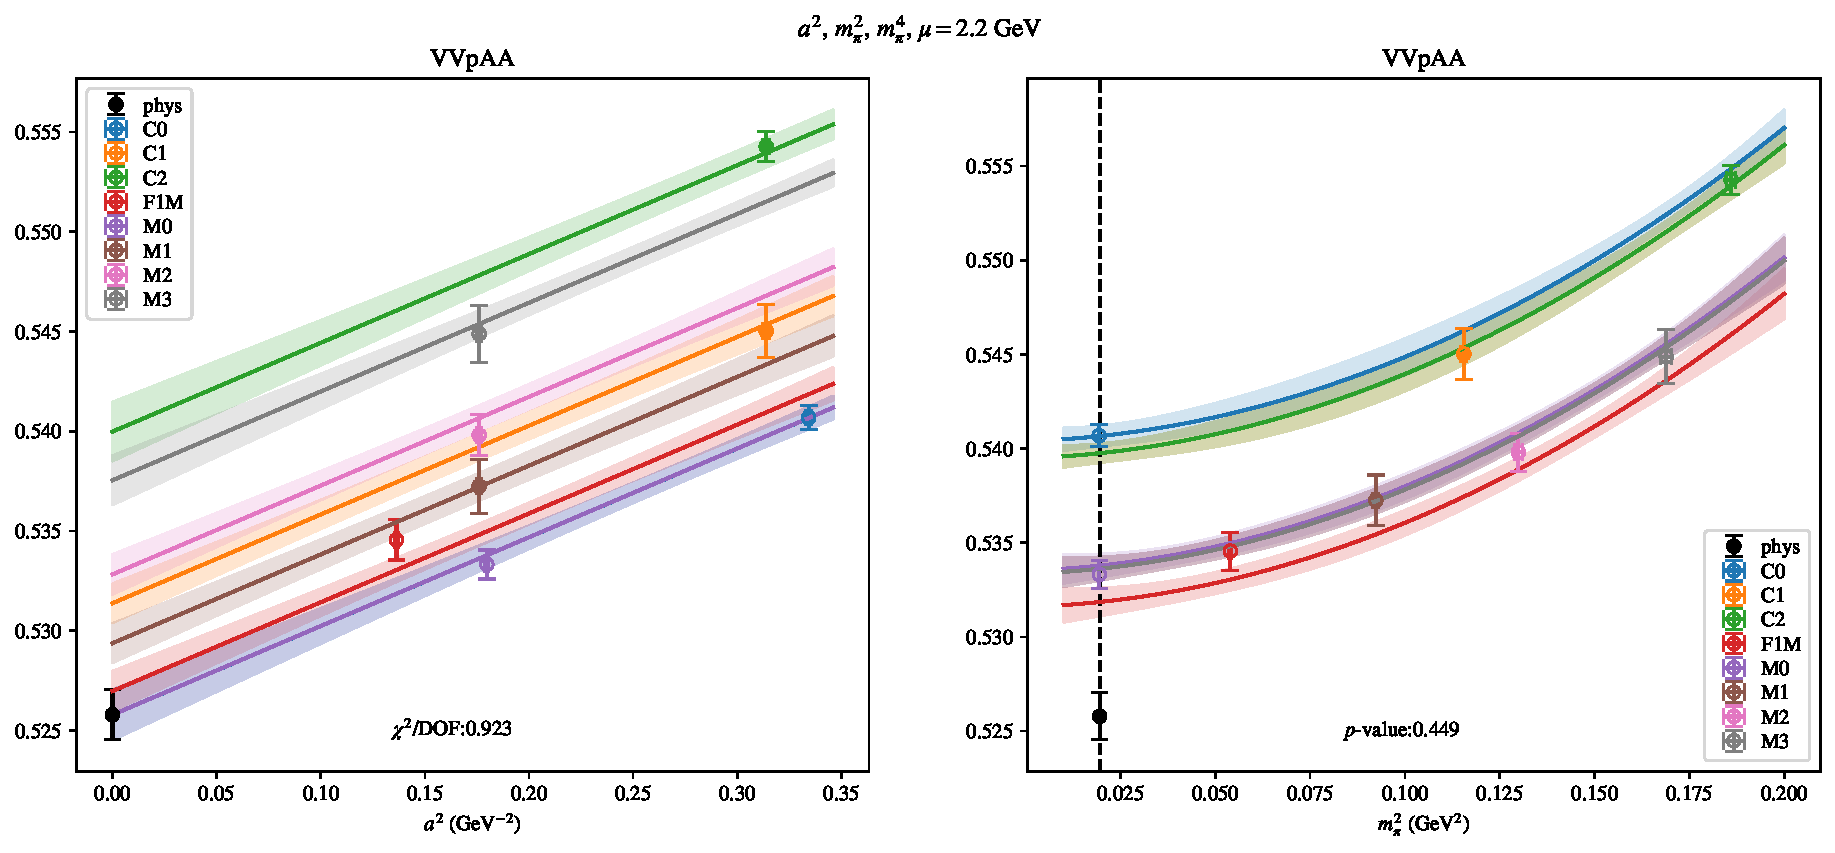
\includepdf[link, pages=-]{VVpAA/SUSY/a2m2m4_22.pdf}
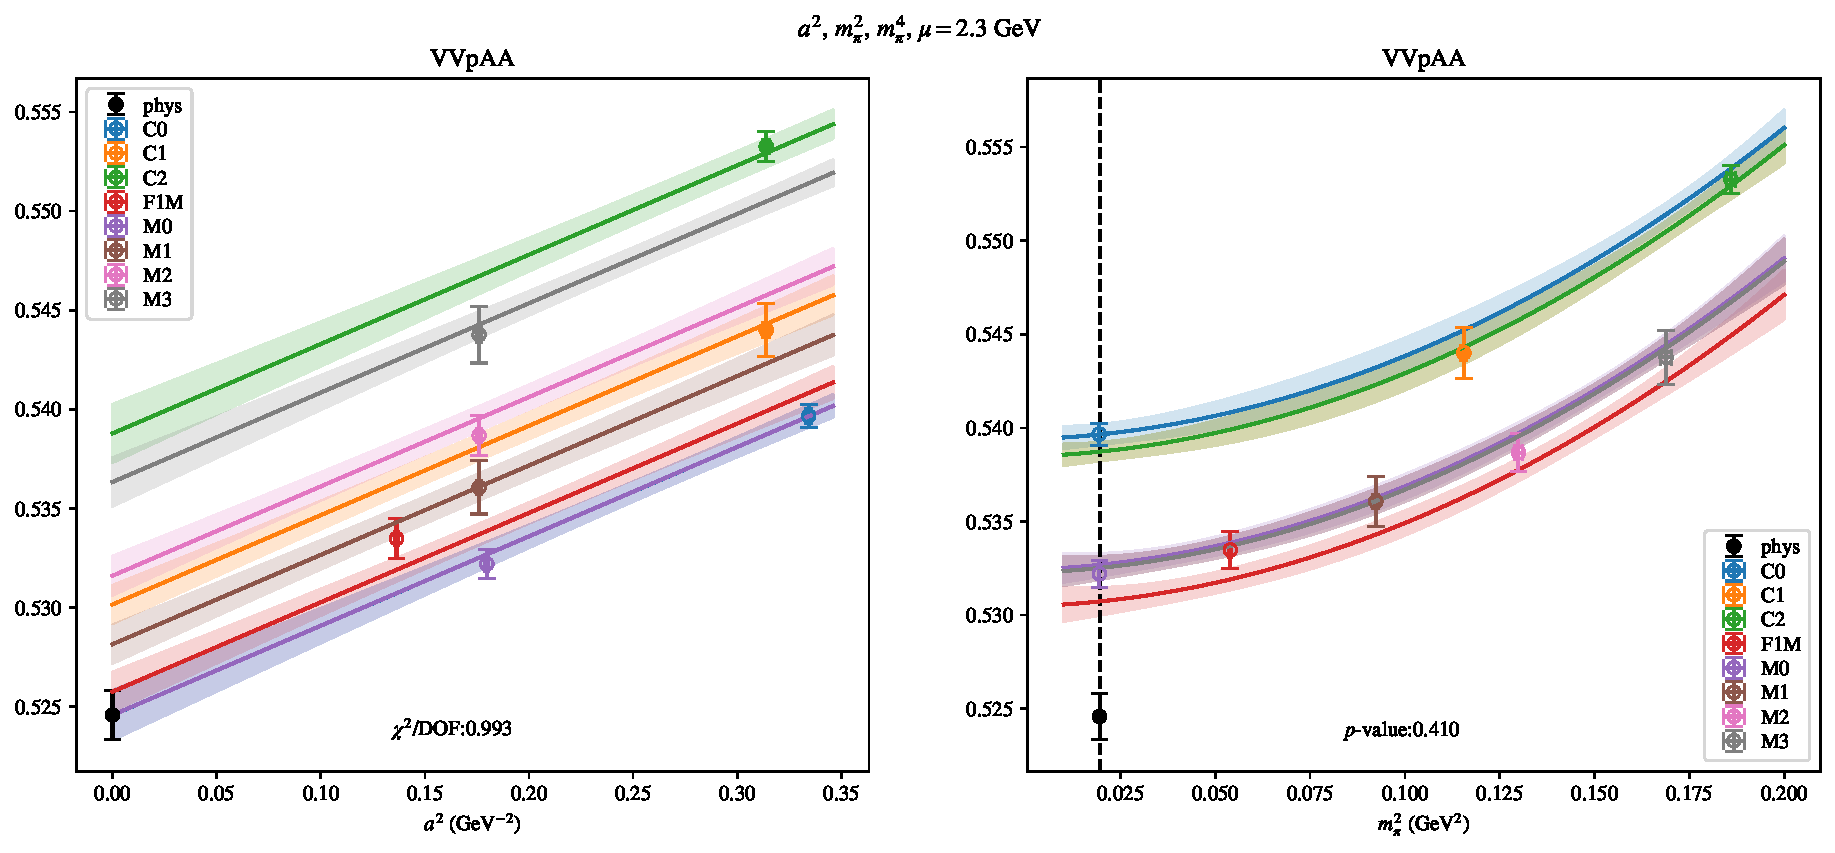
\includepdf[link, pages=-]{VVpAA/SUSY/a2m2m4_23.pdf}
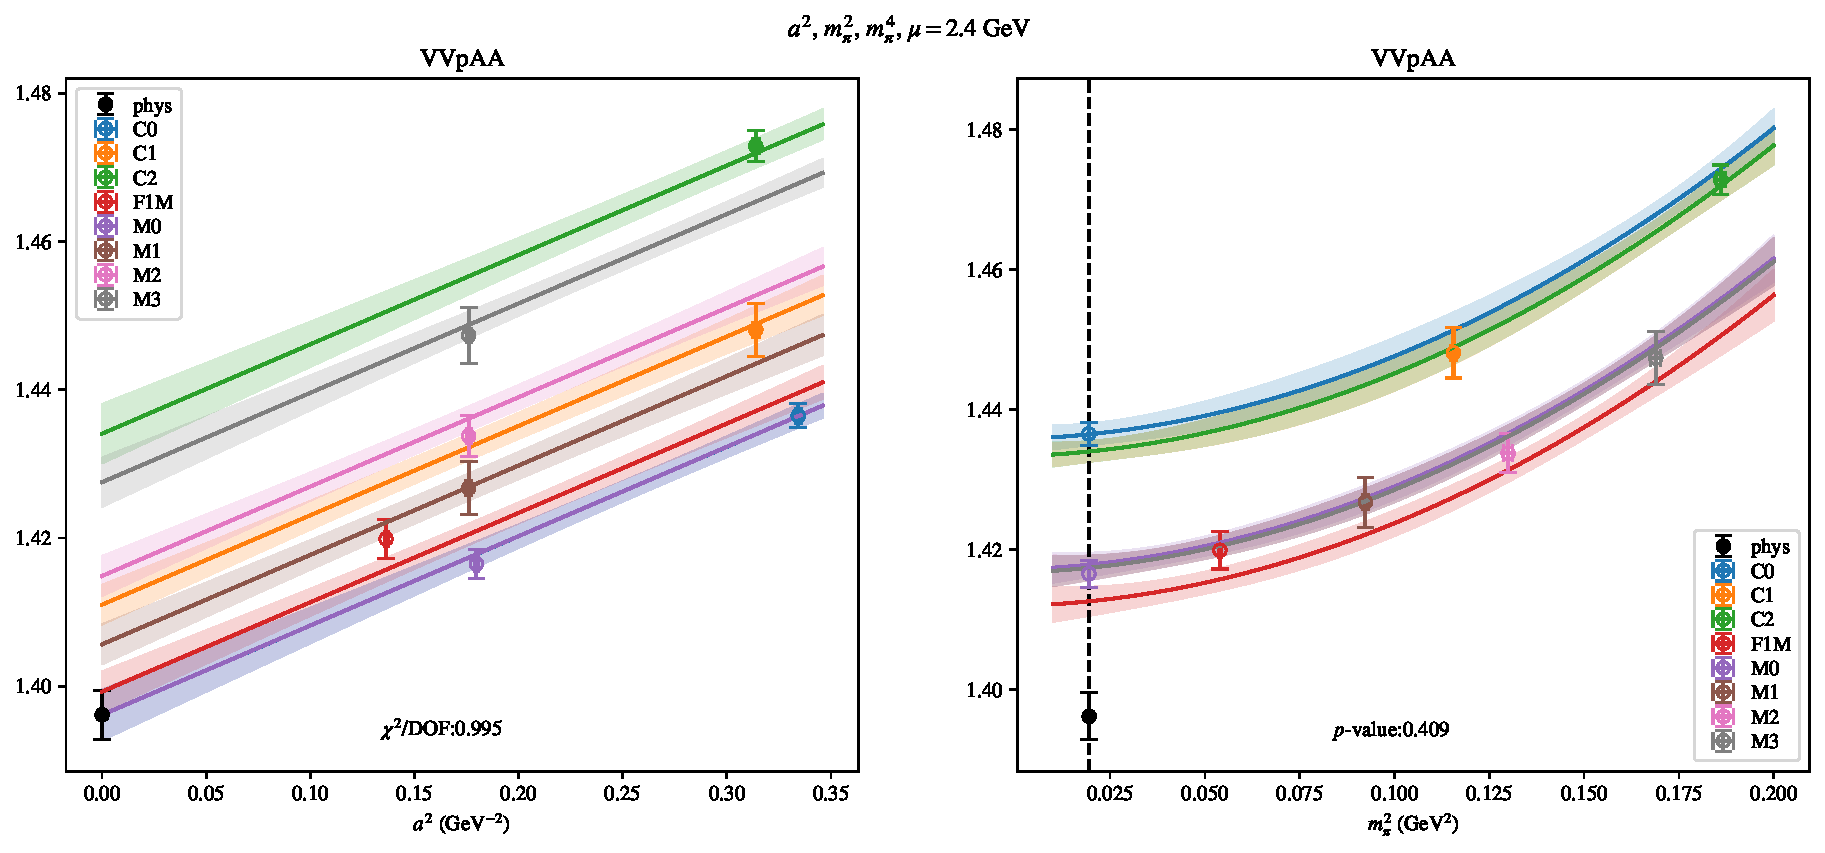
\includepdf[link, pages=-]{VVpAA/SUSY/a2m2m4_24.pdf}
\clearpage
\section{$B_2$}
\begin{table}[h!]
\begin{center}
\begin{tabular}{|c|c|c|c|c|c|}
\hline
$\mu$ (GeV) & $a^2$, $m_\pi^2$& $a^2$, $m_\pi^2$ (no C)& $a^2$, $a^4$, $m_\pi^2$& $a^2$, $m_\pi^2$ (no M3, C2)& $a^2$, $m_\pi^2$, $m_\pi^4$\\
\hline
2.0& \hyperlink{VVmAA/SUSY/a2m2_20.pdf.1}{\textbf{0.56578(95)}: 5.496 (0.0)} & \hyperlink{VVmAA/SUSY/a2m2noC_20.pdf.1}{\textbf{0.5920(52)}: 0.746 (0.474)} & \hyperlink{VVmAA/SUSY/a2a4m2_20.pdf.1}{\textbf{0.6035(85)}: 2.308 (0.056)} & \hyperlink{VVmAA/SUSY/a2m2mcut_20.pdf.1}{\textbf{0.56535(99)}: 7.896 (0.0)} & \hyperlink{VVmAA/SUSY/a2m2m4_20.pdf.1}{\textbf{0.5643(10)}: 4.612 (0.001)}\\
2.2& \hyperlink{VVmAA/SUSY/a2m2_22.pdf.1}{\textbf{0.54762(97)}: 5.529 (0.0)} & \hyperlink{VVmAA/SUSY/a2m2noC_22.pdf.1}{\textbf{0.5728(51)}: 1.04 (0.353)} & \hyperlink{VVmAA/SUSY/a2a4m2_22.pdf.1}{\textbf{0.5802(83)}: 3.438 (0.008)} & \hyperlink{VVmAA/SUSY/a2m2mcut_22.pdf.1}{\textbf{0.5473(10)}: 7.756 (0.0)} & \hyperlink{VVmAA/SUSY/a2m2m4_22.pdf.1}{\textbf{0.54634(99)}: 4.674 (0.001)}\\
2.3& \hyperlink{VVmAA/SUSY/a2m2_23.pdf.1}{\textbf{0.53989(93)}: 5.578 (0.0)} & \hyperlink{VVmAA/SUSY/a2m2noC_23.pdf.1}{\textbf{0.5646(50)}: 1.222 (0.295)} & \hyperlink{VVmAA/SUSY/a2a4m2_23.pdf.1}{\textbf{0.5721(82)}: 3.356 (0.009)} & \hyperlink{VVmAA/SUSY/a2m2mcut_23.pdf.1}{\textbf{0.53960(97)}: 7.889 (0.0)} & \hyperlink{VVmAA/SUSY/a2m2m4_23.pdf.1}{\textbf{0.53866(96)}: 4.739 (0.001)}\\
2.4& \hyperlink{VVmAA/SUSY/a2m2_24.pdf.1}{\textbf{0.53375(91)}: 5.117 (0.0)} & \hyperlink{VVmAA/SUSY/a2m2noC_24.pdf.1}{\textbf{0.5558(49)}: 1.203 (0.3)} & \hyperlink{VVmAA/SUSY/a2a4m2_24.pdf.1}{\textbf{0.5610(80)}: 3.681 (0.005)} & \hyperlink{VVmAA/SUSY/a2m2mcut_24.pdf.1}{\textbf{0.53353(97)}: 7.248 (0.0)} & \hyperlink{VVmAA/SUSY/a2m2m4_24.pdf.1}{\textbf{0.53256(96)}: 4.519 (0.001)}\\
\hline
\end{tabular}
\caption{Physical point value from chiral and continuum extrapolation at renormalisation scale $\mu$. Entries are \textbf{value(error)}: $\chi^2/\text{DOF}$ ($p$-value).}
\end{center}
\end{table}
\begin{table}[h!]
\begin{center}
\begin{tabular}{|c c|c|c|c|c|c|}
\hline
$\mu$ (GeV) &  & $a^2$, $m_\pi^2$& $a^2$, $m_\pi^2$ (no C)& $a^2$, $a^4$, $m_\pi^2$& $a^2$, $m_\pi^2$ (no M3, C2)& $a^2$, $m_\pi^2$, $m_\pi^4$\\
\hline
\multirow{2}{0.5in}{2.0} & $\alpha$ & 0.1118(60)& -0.14(50)& -0.4(12)& 0.1139(65)& 0.1200(65)\\
 & $\beta$ & 0.00726(17)& 0.00682(25)& 0.00701(16)& 0.00771(27)& 0.00976(69)\\
\hline
\multirow{2}{0.5in}{2.2} & $\alpha$ & 0.1318(63)& -0.12(50)& -0.3(12)& 0.1331(67)& 0.1394(66)\\
 & $\beta$ & 0.00693(14)& 0.00641(23)& 0.00673(14)& 0.00740(26)& 0.00936(72)\\
\hline
\multirow{2}{0.5in}{2.3} & $\alpha$ & 0.1426(64)& -0.11(50)& -0.3(12)& 0.1439(67)& 0.1501(67)\\
 & $\beta$ & 0.00688(15)& 0.00637(23)& 0.00668(14)& 0.00732(26)& 0.00925(71)\\
\hline
\multirow{2}{0.5in}{2.4} & $\alpha$ & 0.1481(63)& -0.08(50)& -0.2(12)& 0.1489(68)& 0.1554(68)\\
 & $\beta$ & 0.00686(13)& 0.00634(21)& 0.00669(13)& 0.00723(24)& 0.00896(67)\\
\hline
\end{tabular}
\caption{Fit values of coefficients in $B = B_{phys} + \mathbf{\alpha} a^2 + \mathbf{\beta}\left(\frac{m_\pi^2}{f_\pi^2}-\frac{m_{\pi,PDG}^2}{f_\pi^2}\right) + \ldots$.}
\end{center}
\end{table}
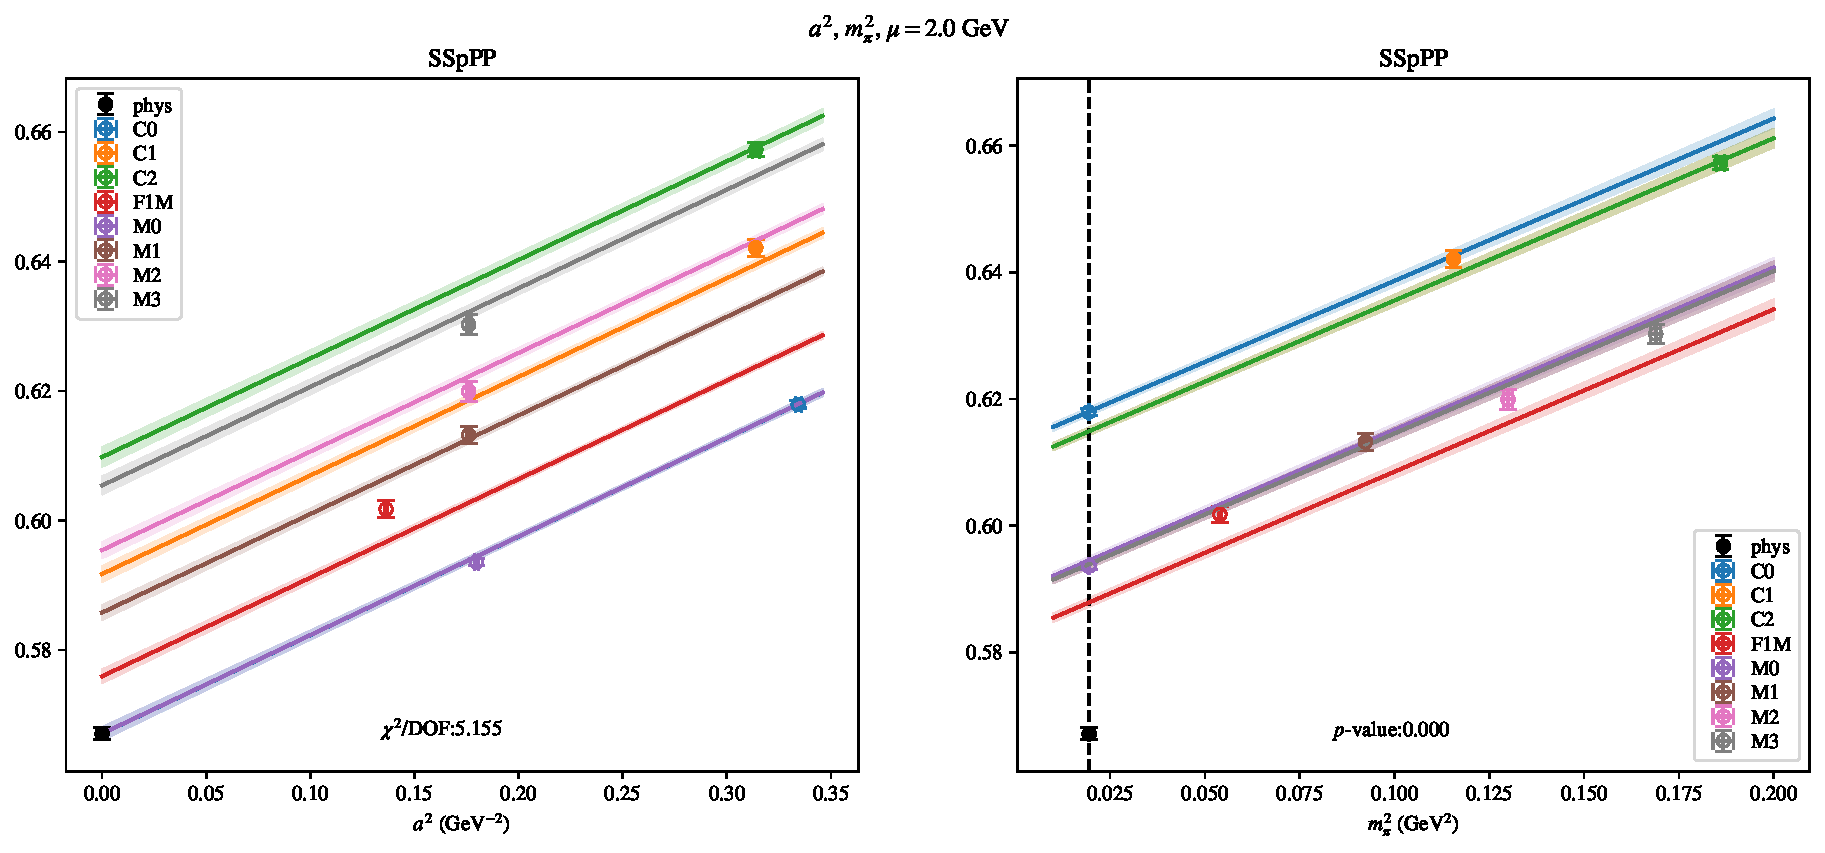
\includepdf[link, pages=-]{VVmAA/SUSY/a2m2_20.pdf}
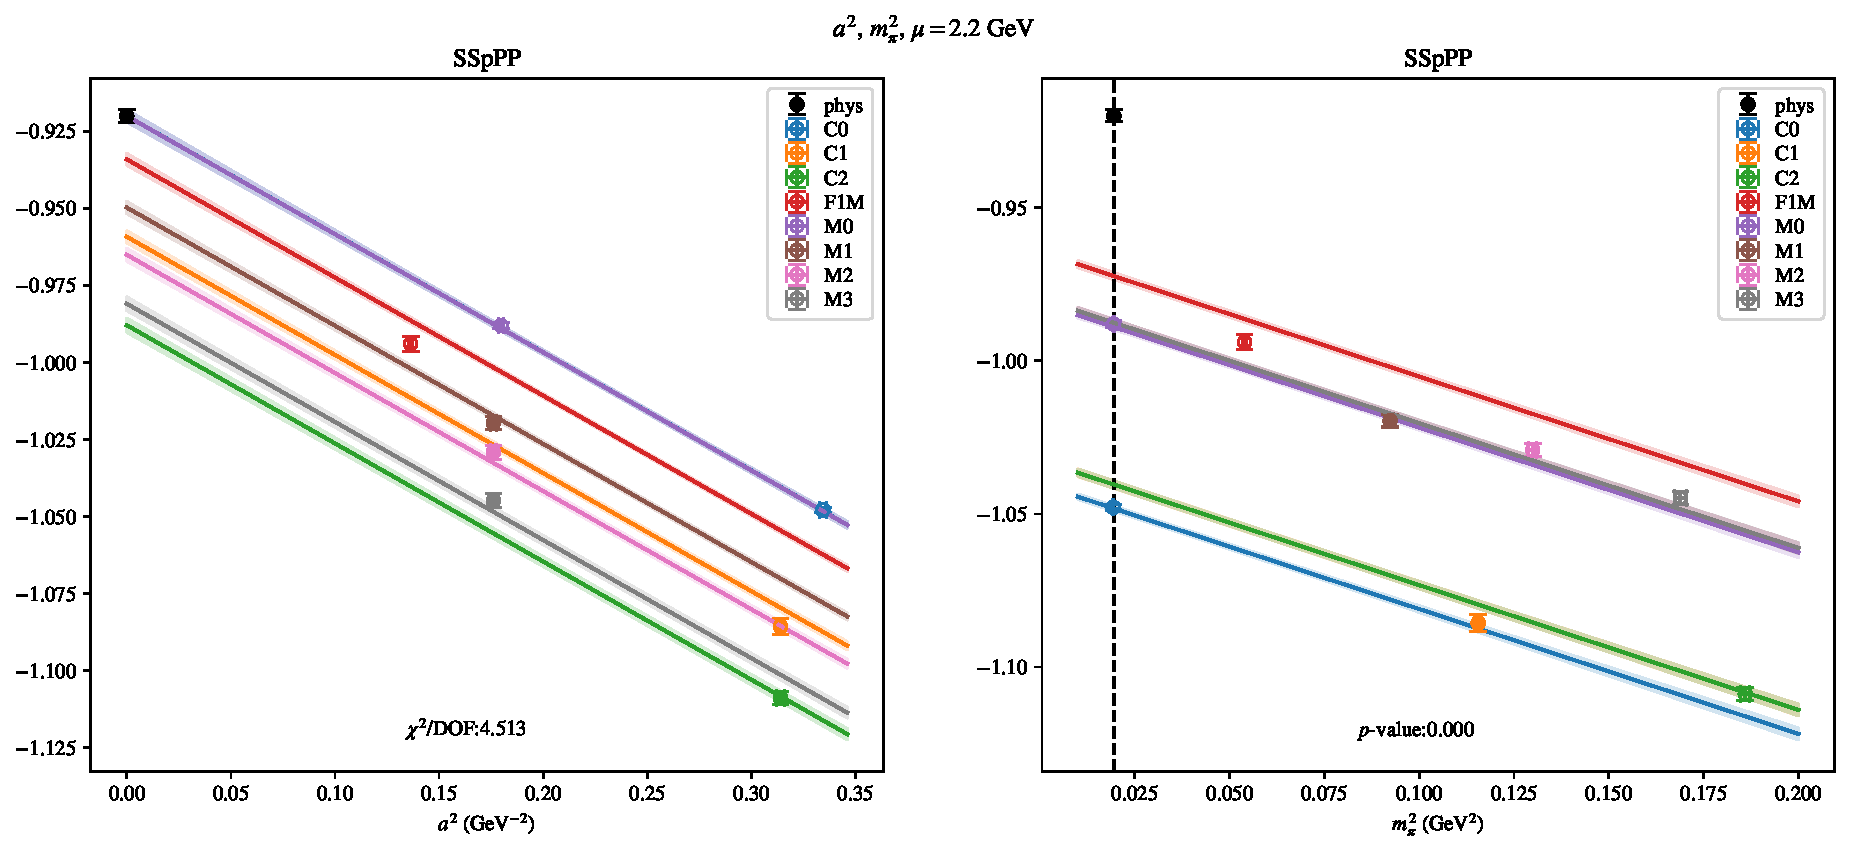
\includepdf[link, pages=-]{VVmAA/SUSY/a2m2_22.pdf}
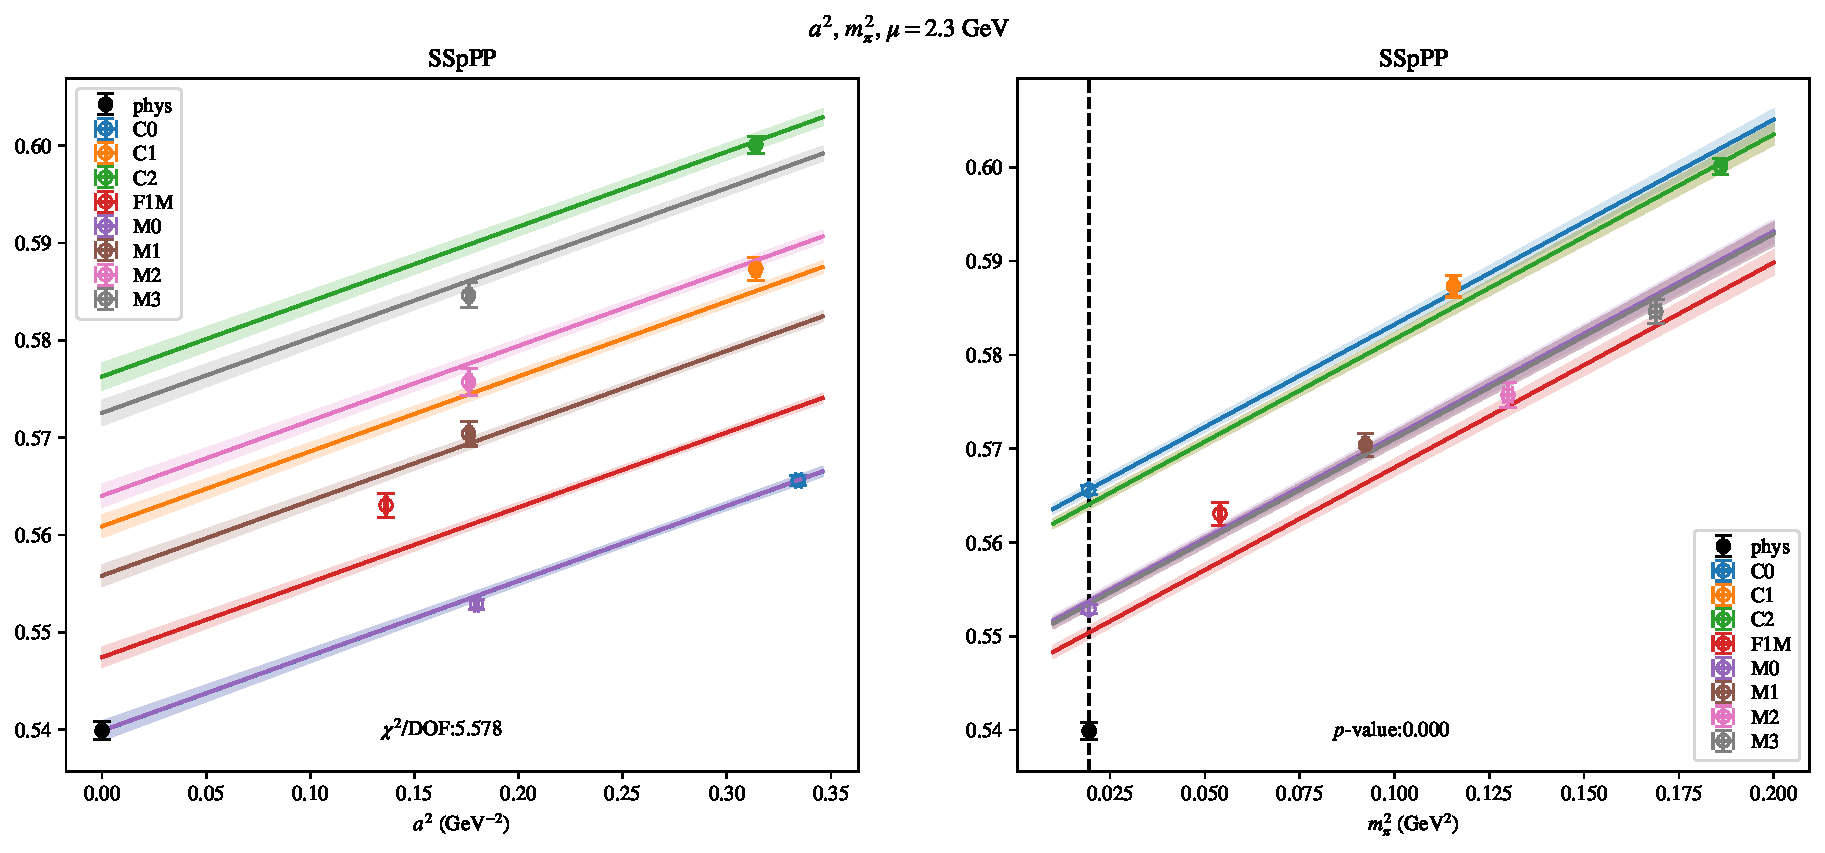
\includepdf[link, pages=-]{VVmAA/SUSY/a2m2_23.pdf}
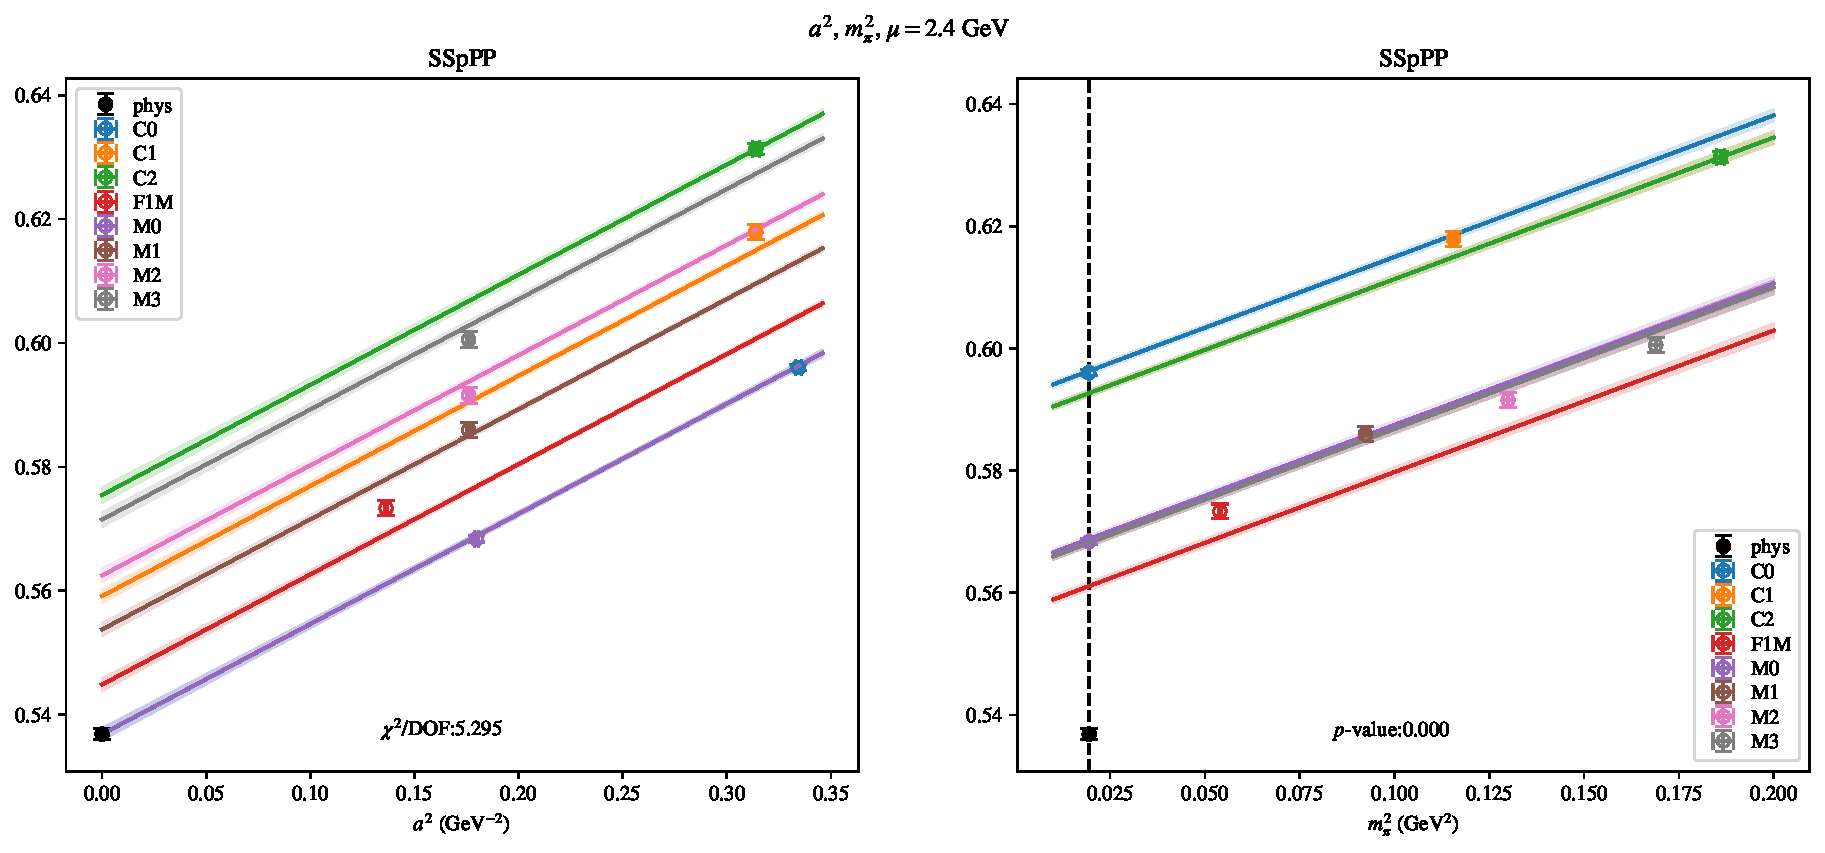
\includepdf[link, pages=-]{VVmAA/SUSY/a2m2_24.pdf}
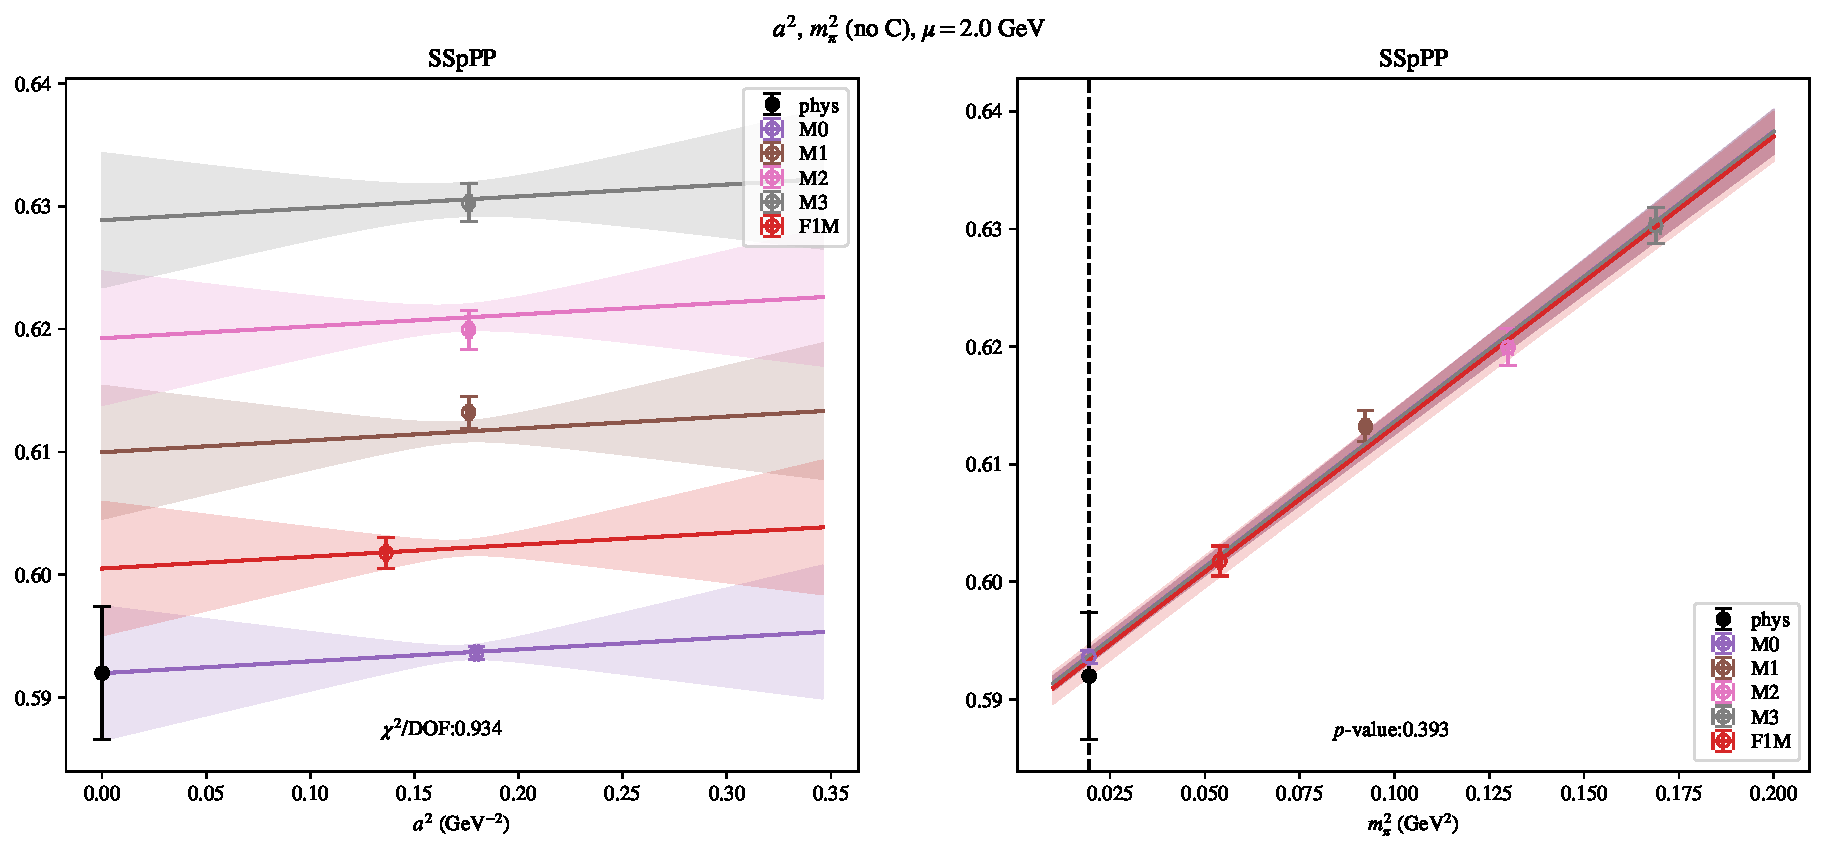
\includepdf[link, pages=-]{VVmAA/SUSY/a2m2noC_20.pdf}
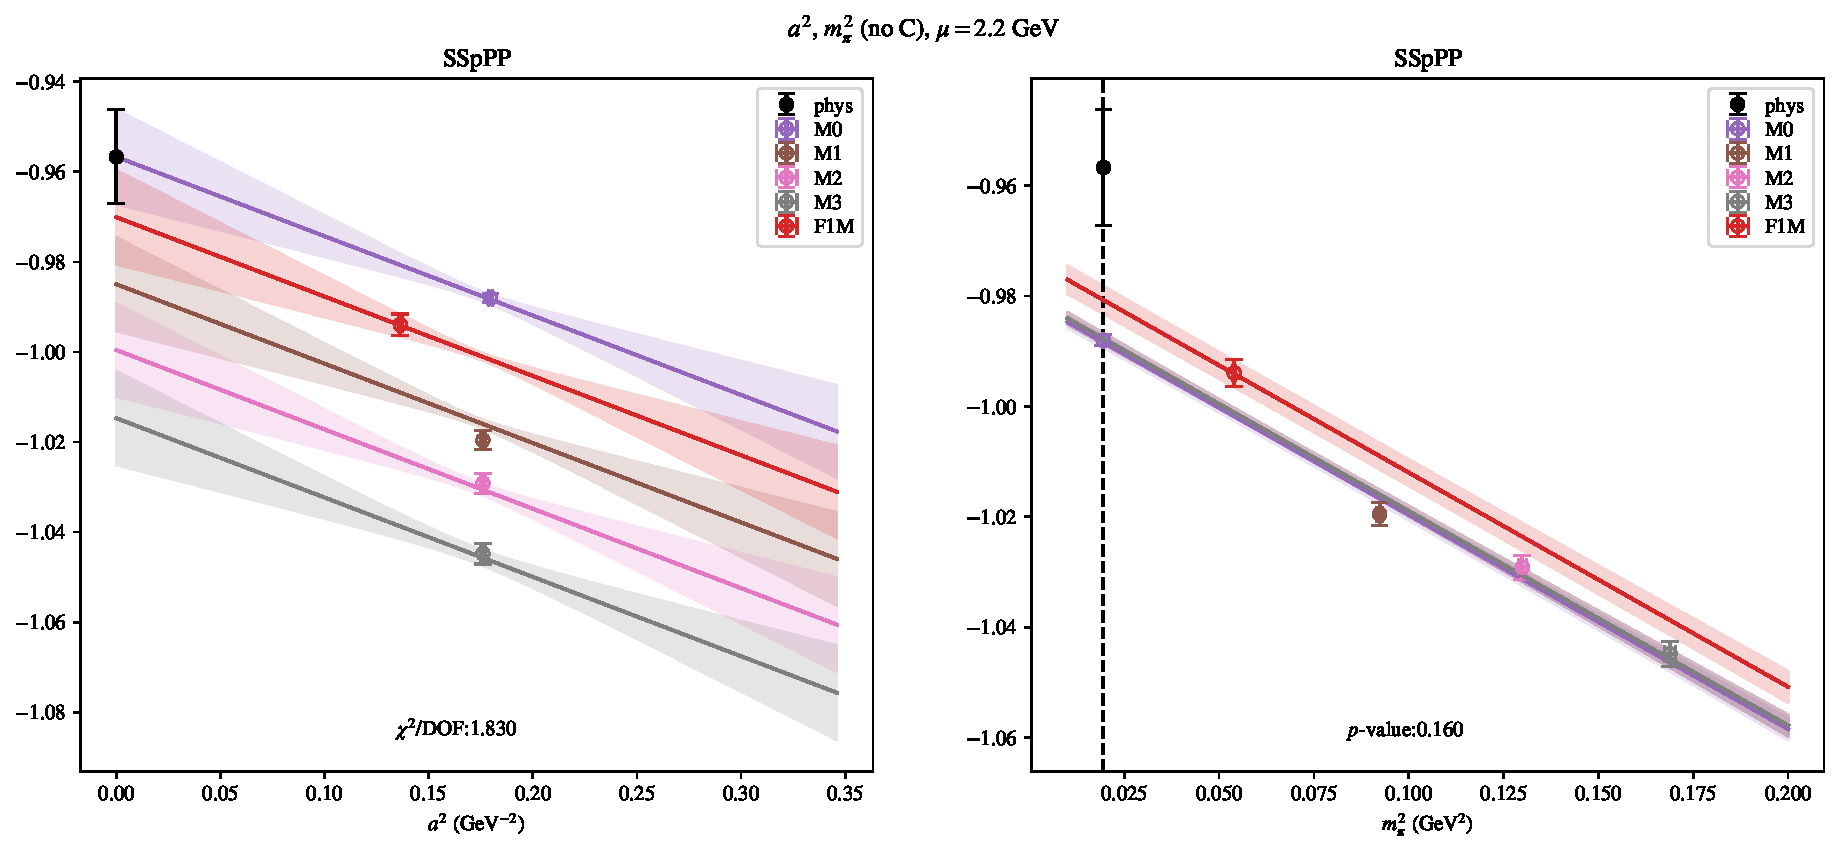
\includepdf[link, pages=-]{VVmAA/SUSY/a2m2noC_22.pdf}
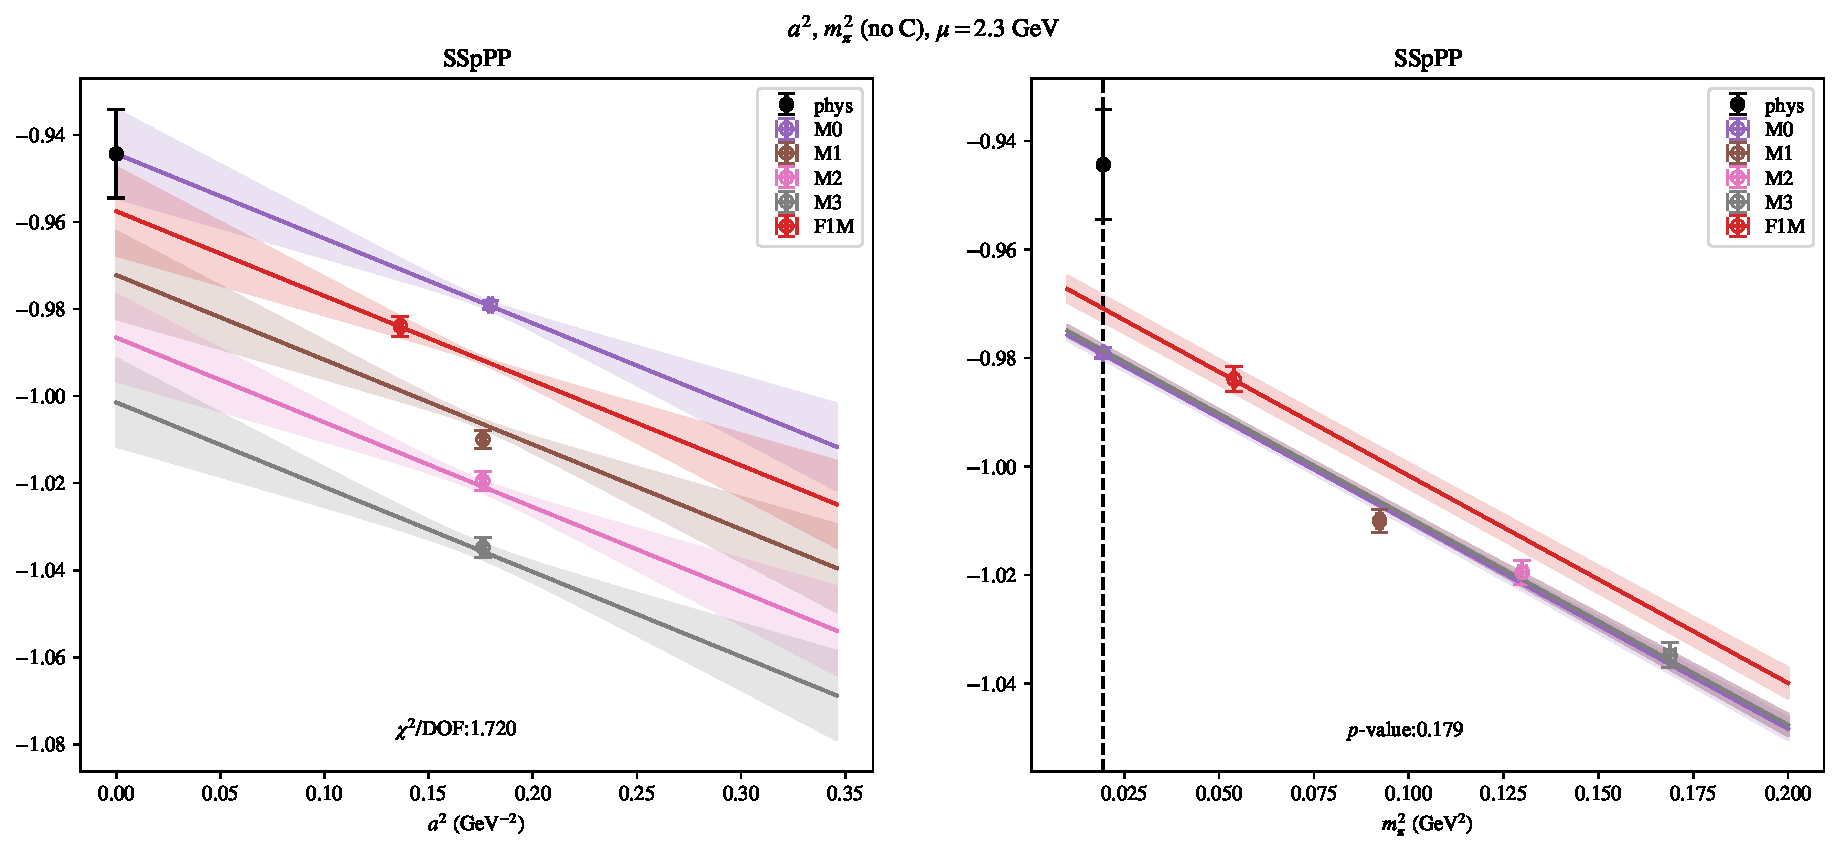
\includepdf[link, pages=-]{VVmAA/SUSY/a2m2noC_23.pdf}
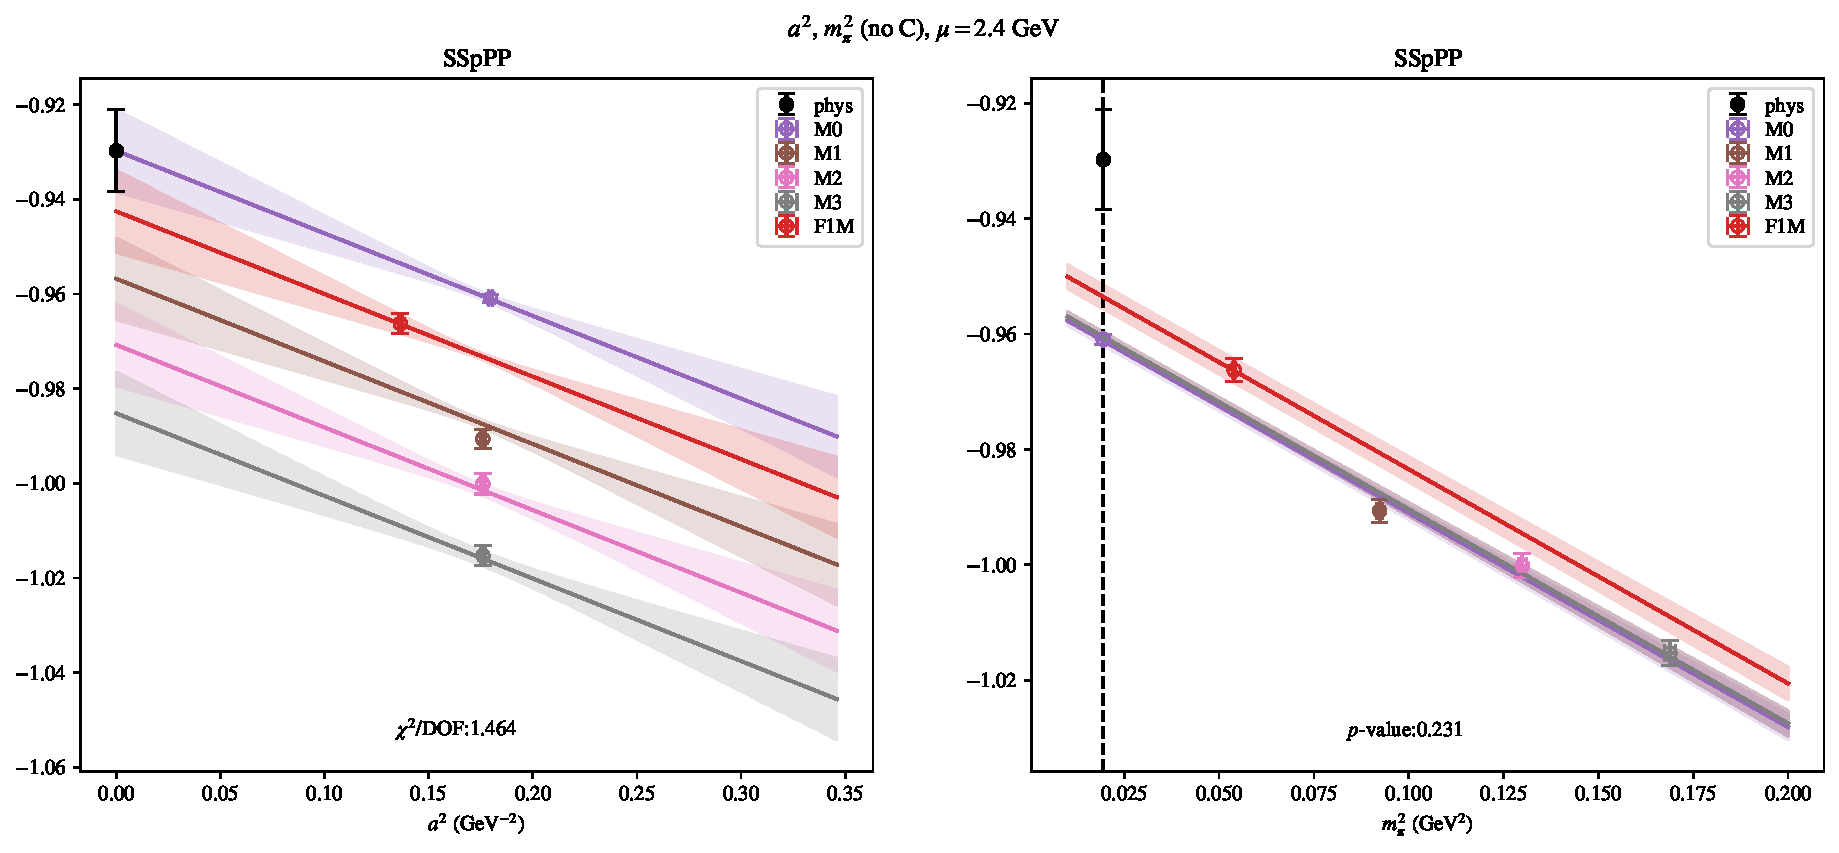
\includepdf[link, pages=-]{VVmAA/SUSY/a2m2noC_24.pdf}
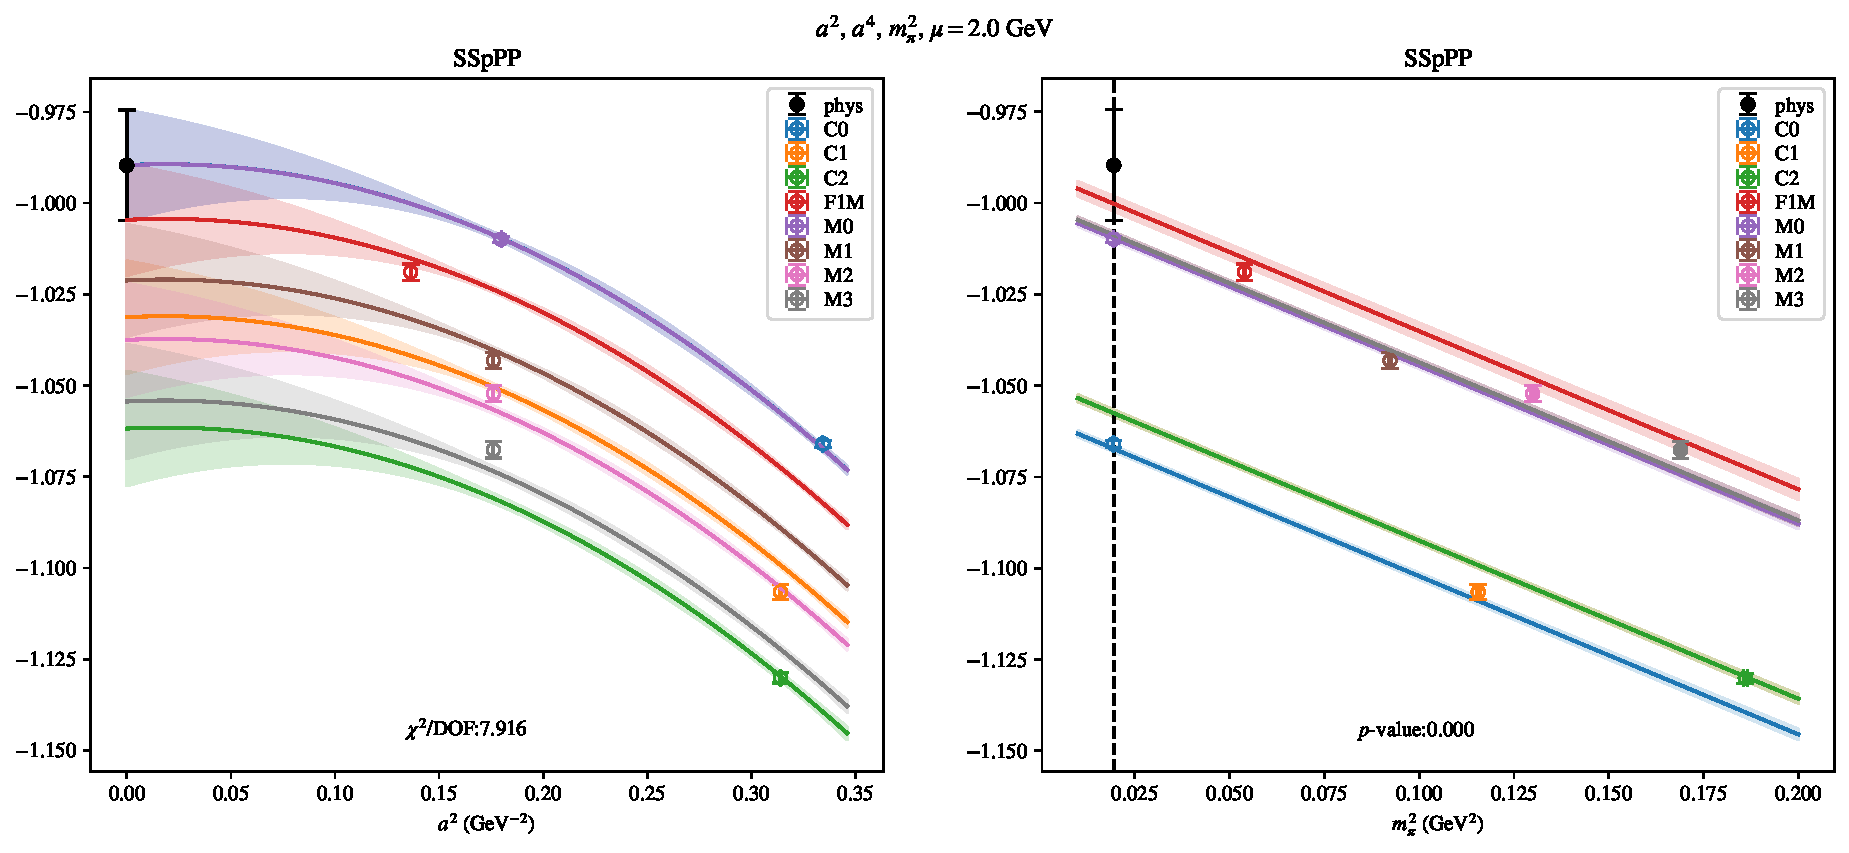
\includepdf[link, pages=-]{VVmAA/SUSY/a2a4m2_20.pdf}
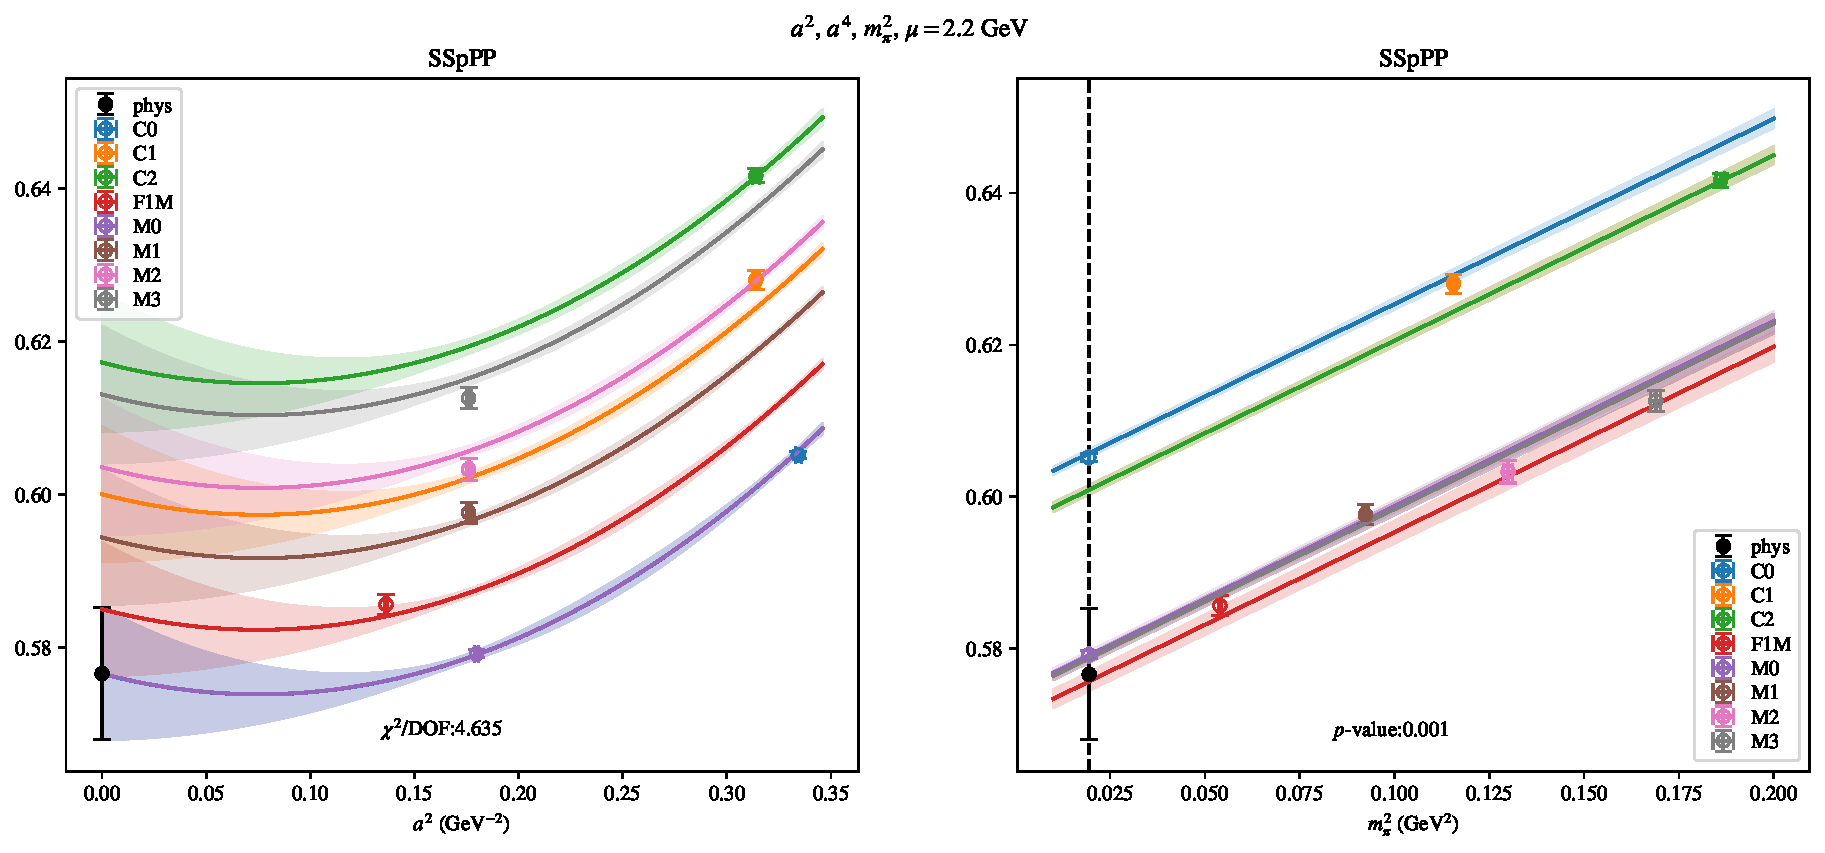
\includepdf[link, pages=-]{VVmAA/SUSY/a2a4m2_22.pdf}
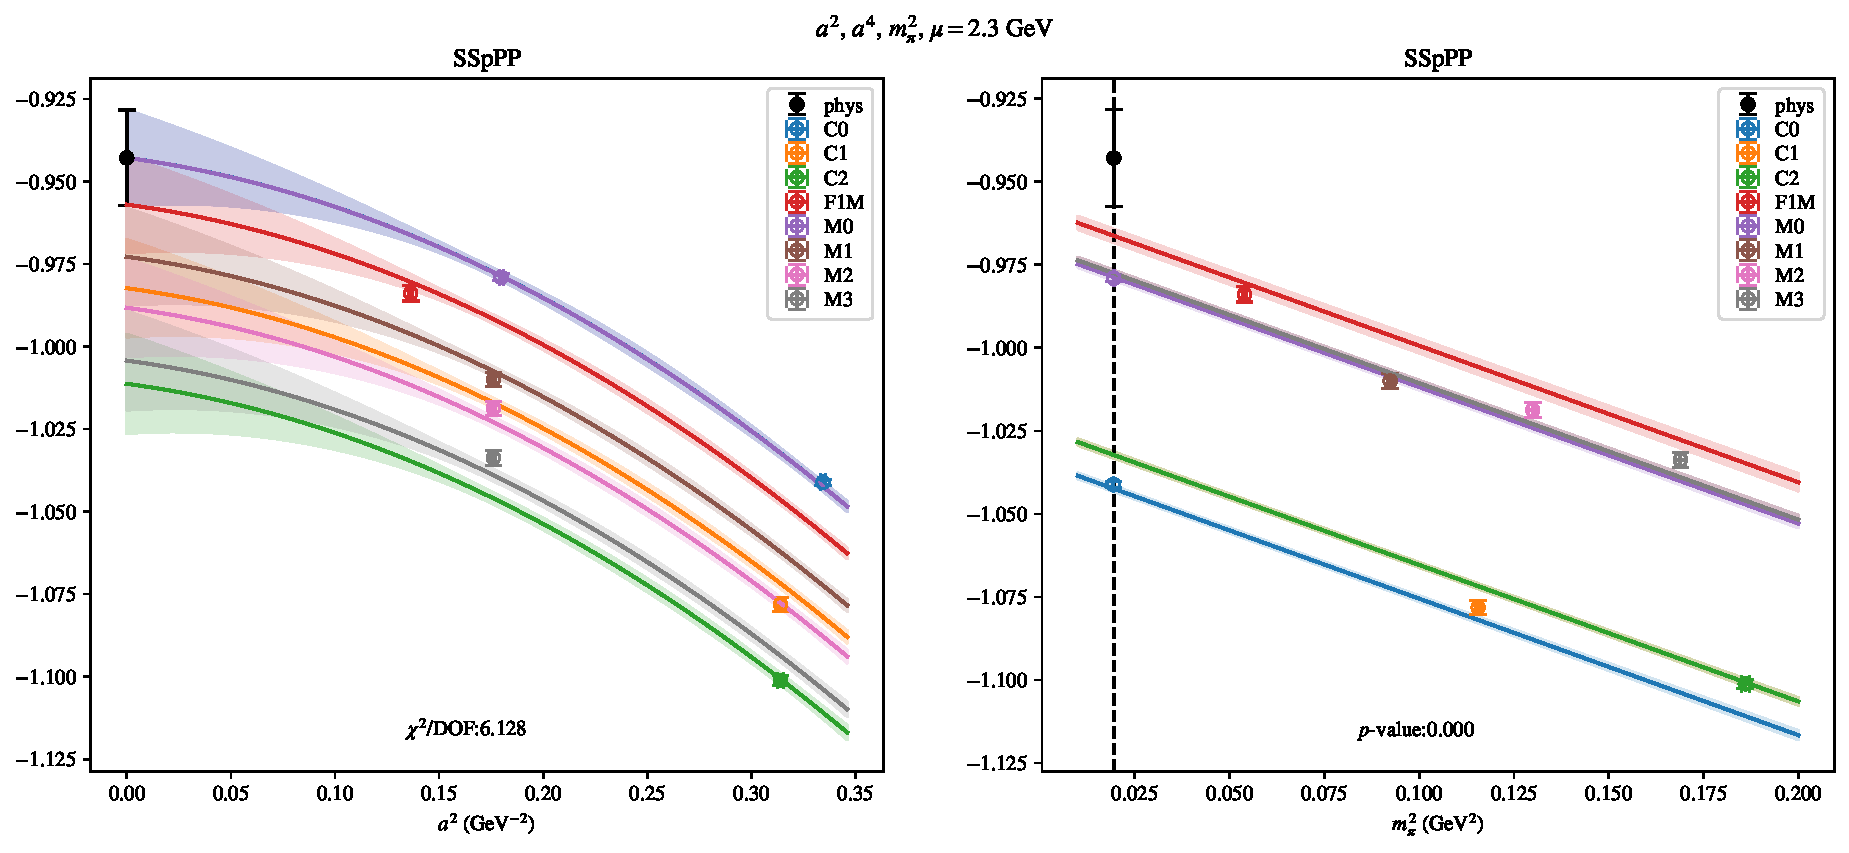
\includepdf[link, pages=-]{VVmAA/SUSY/a2a4m2_23.pdf}
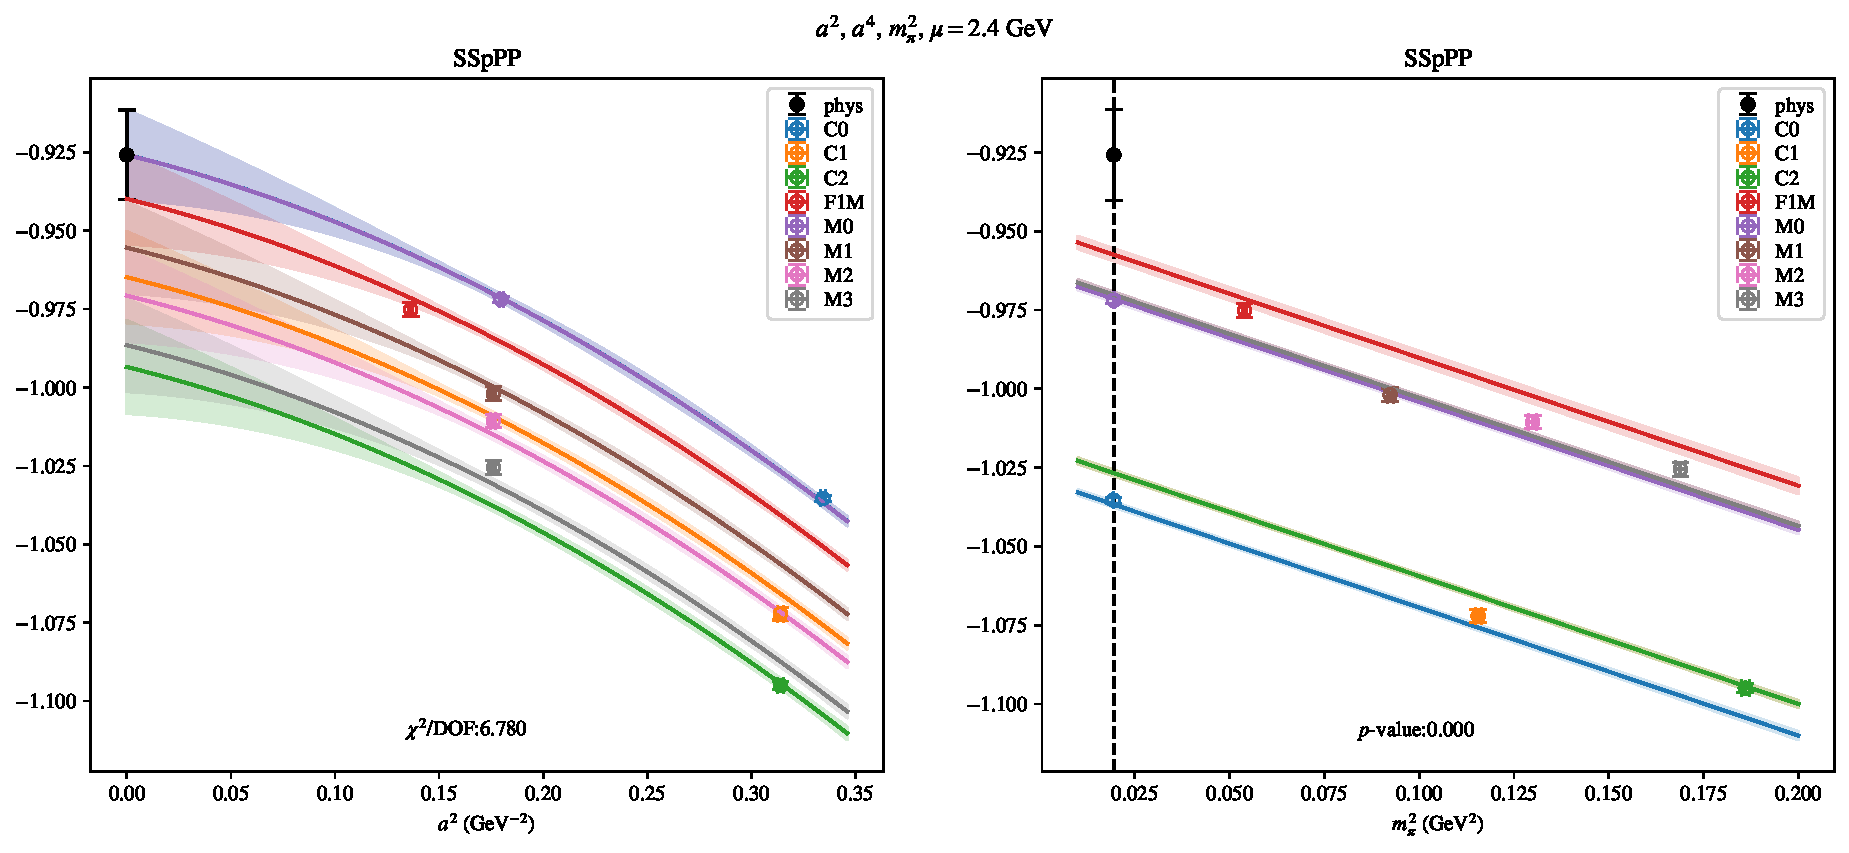
\includepdf[link, pages=-]{VVmAA/SUSY/a2a4m2_24.pdf}
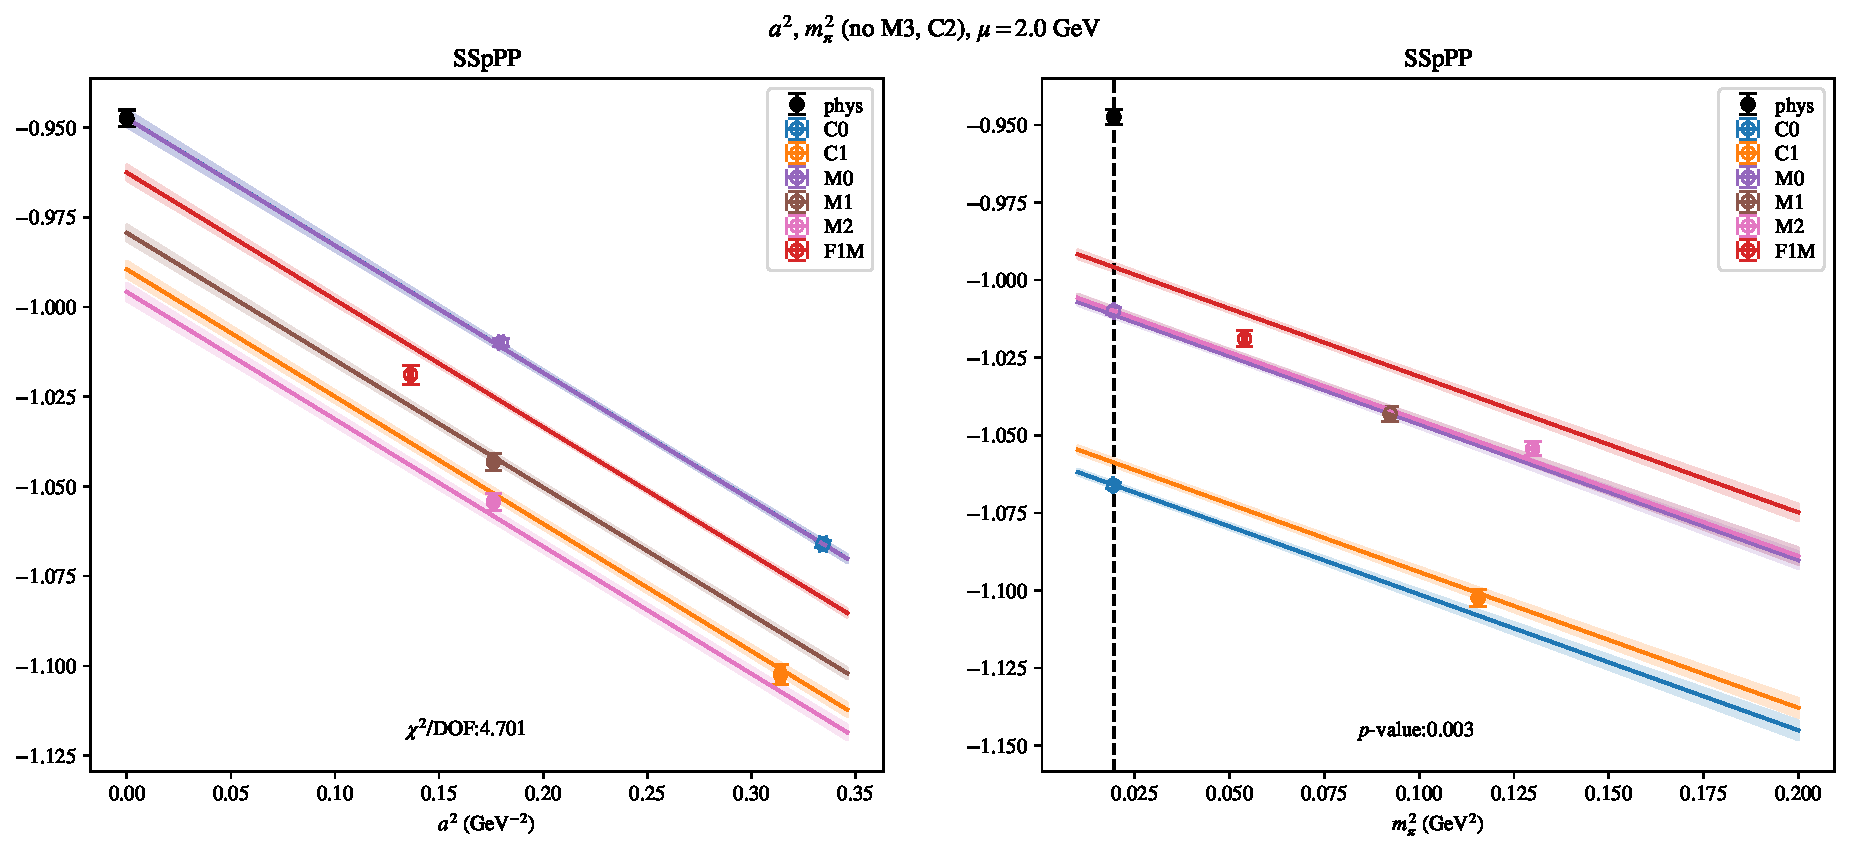
\includepdf[link, pages=-]{VVmAA/SUSY/a2m2mcut_20.pdf}
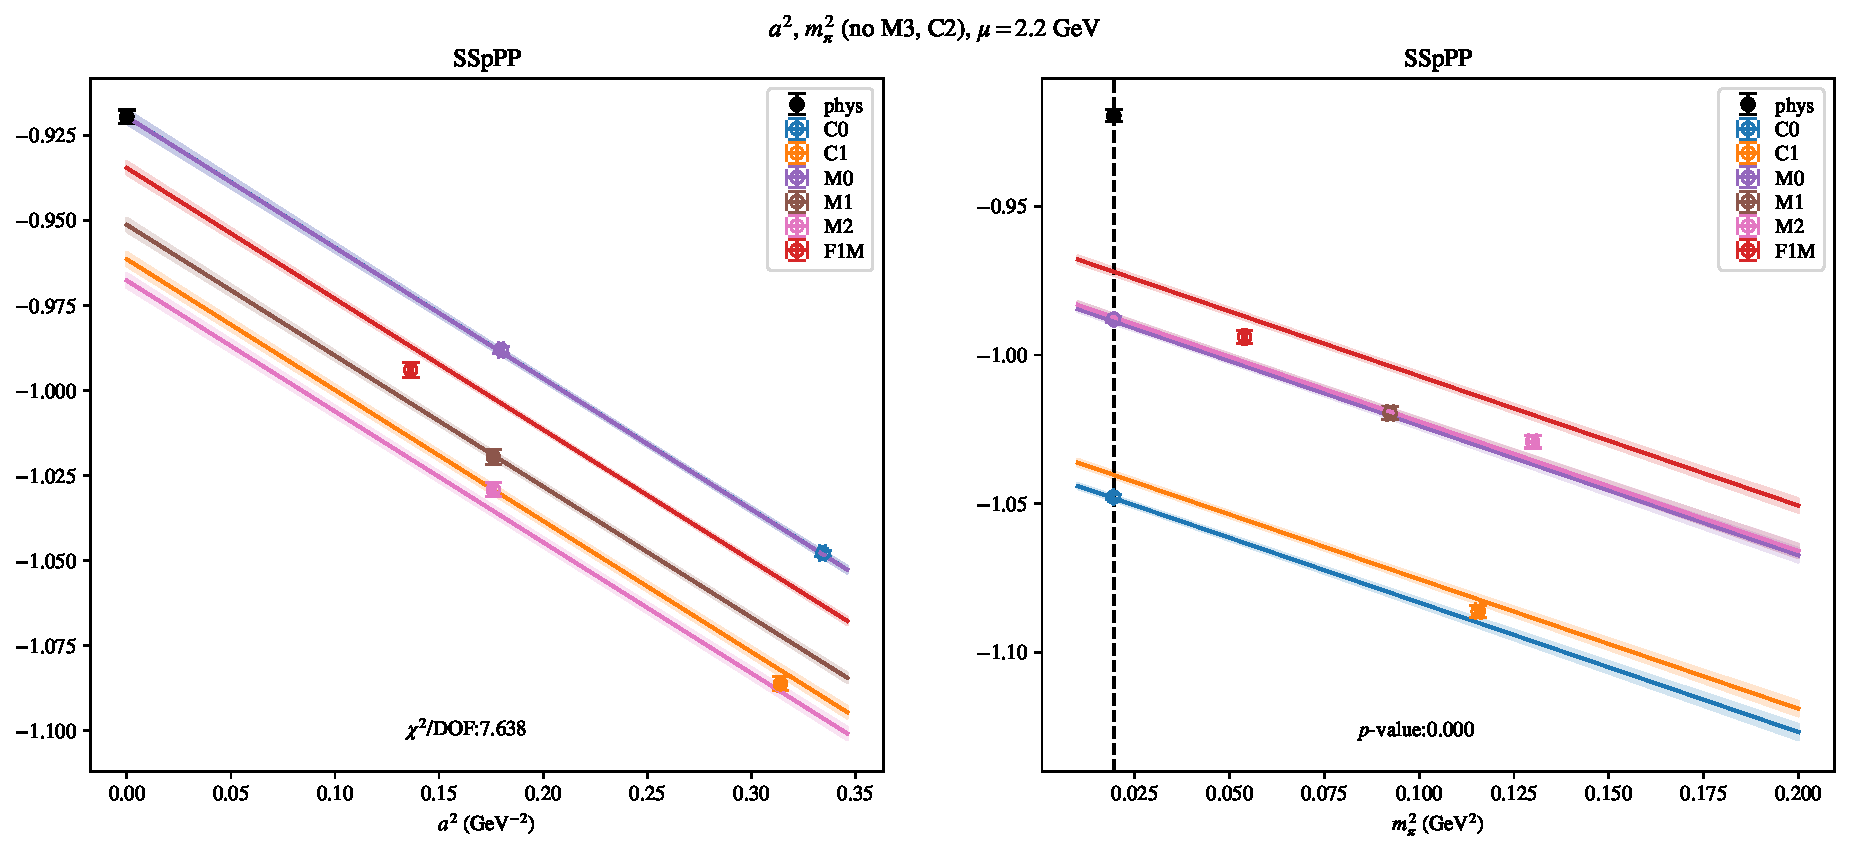
\includepdf[link, pages=-]{VVmAA/SUSY/a2m2mcut_22.pdf}
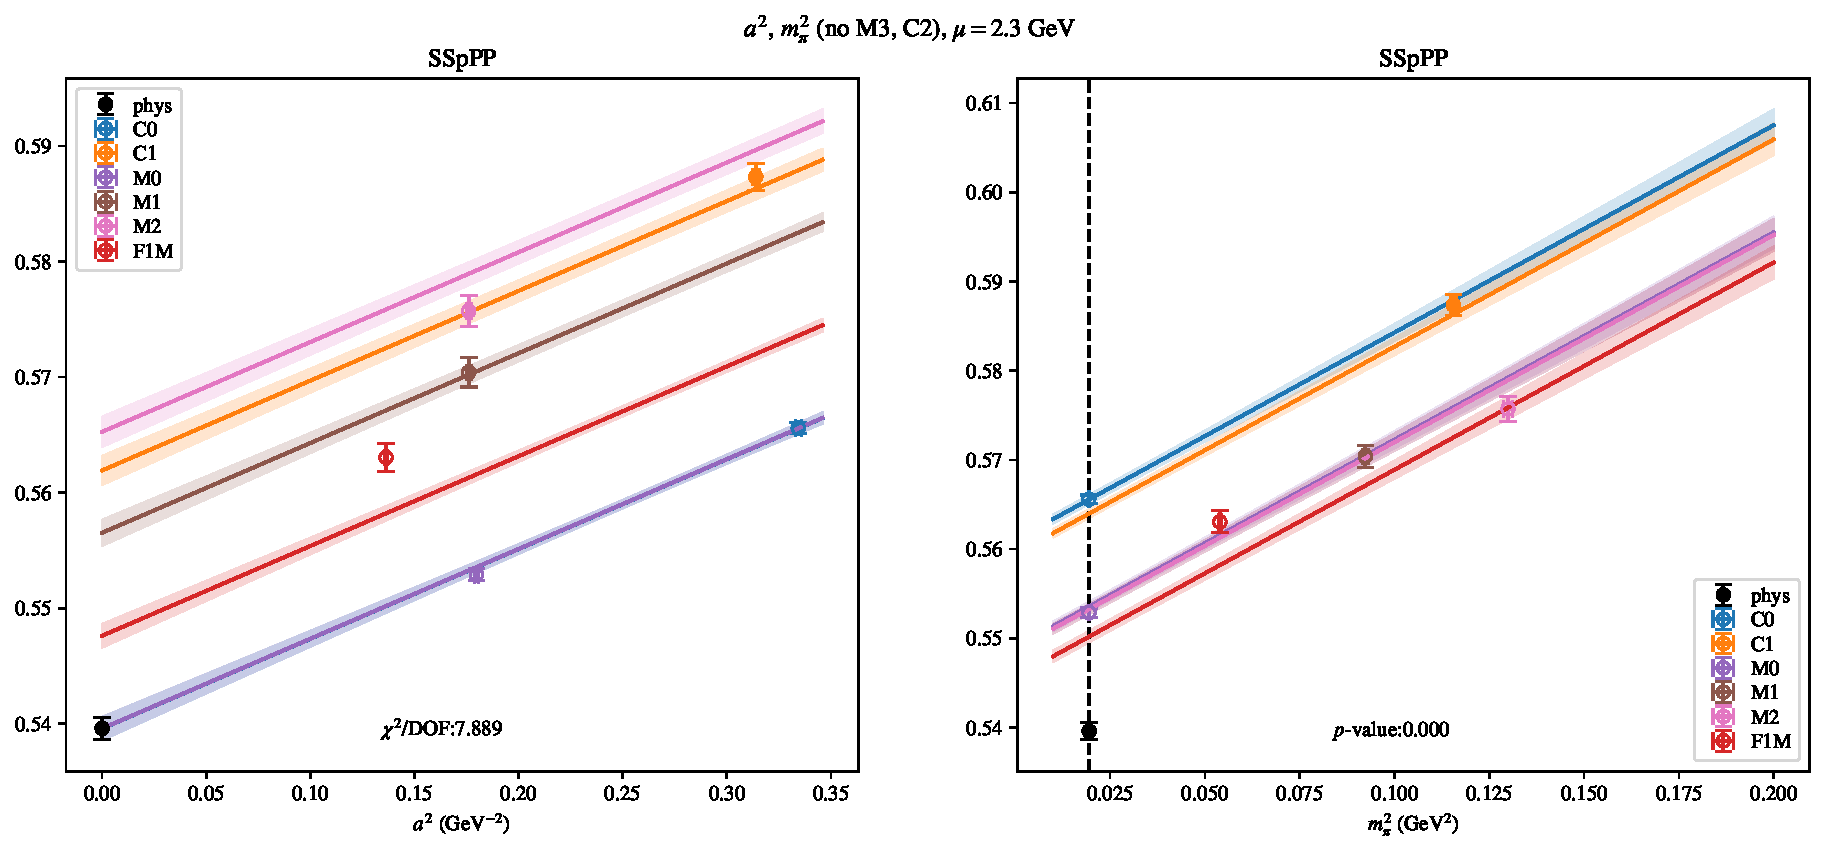
\includepdf[link, pages=-]{VVmAA/SUSY/a2m2mcut_23.pdf}
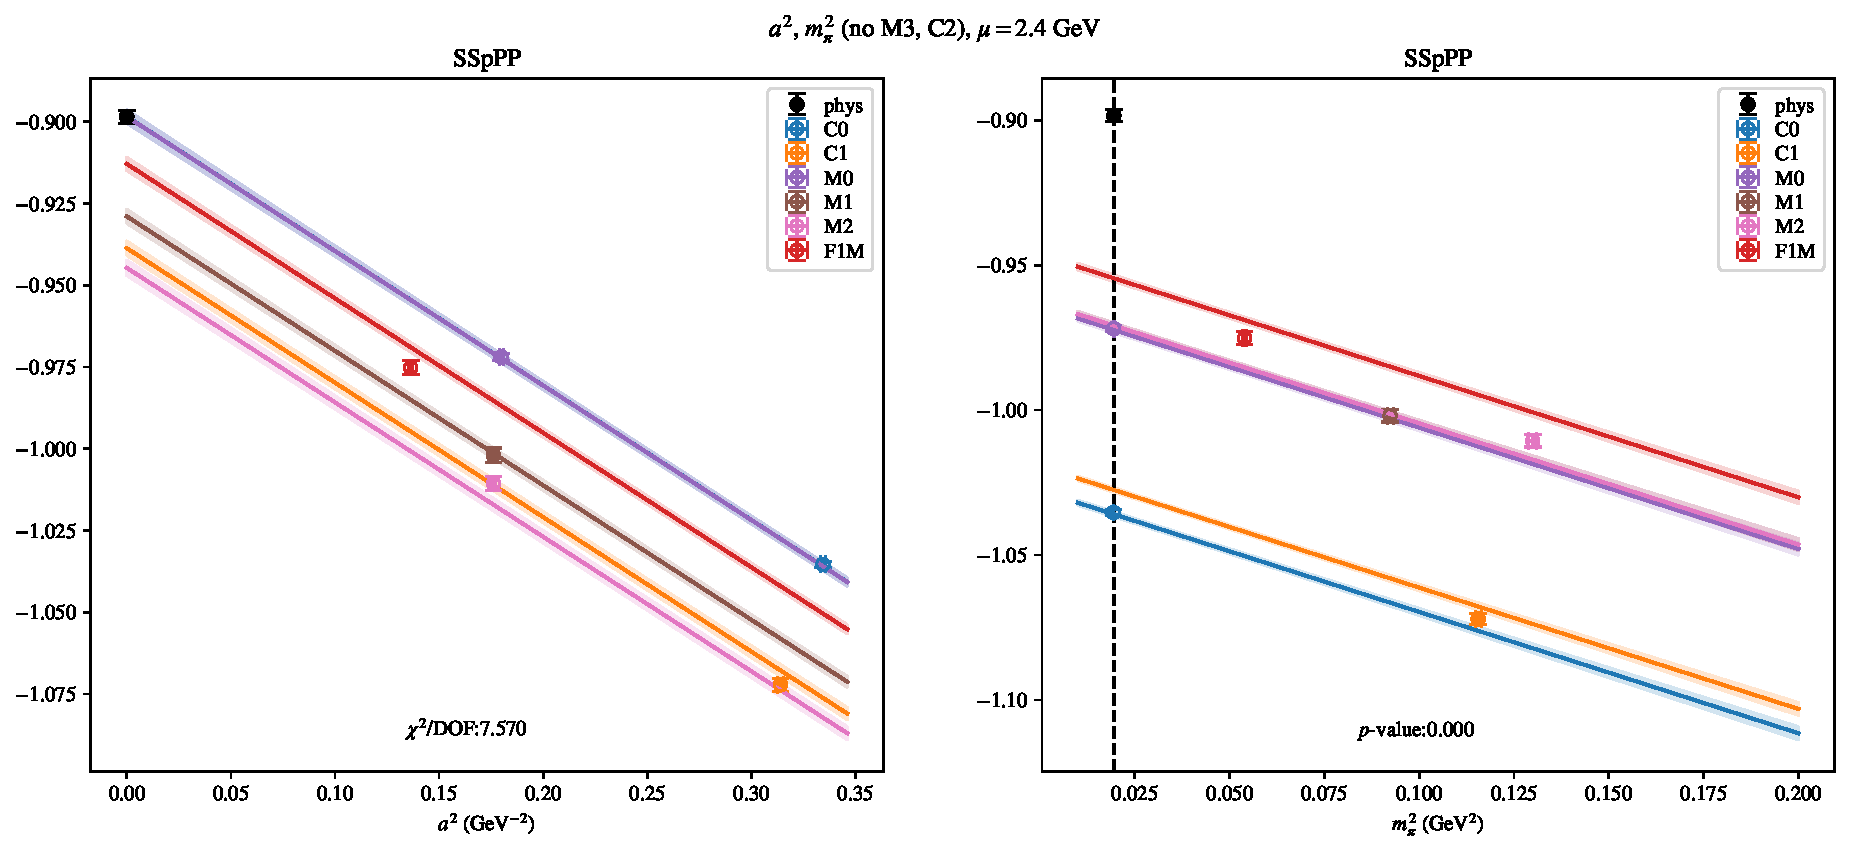
\includepdf[link, pages=-]{VVmAA/SUSY/a2m2mcut_24.pdf}
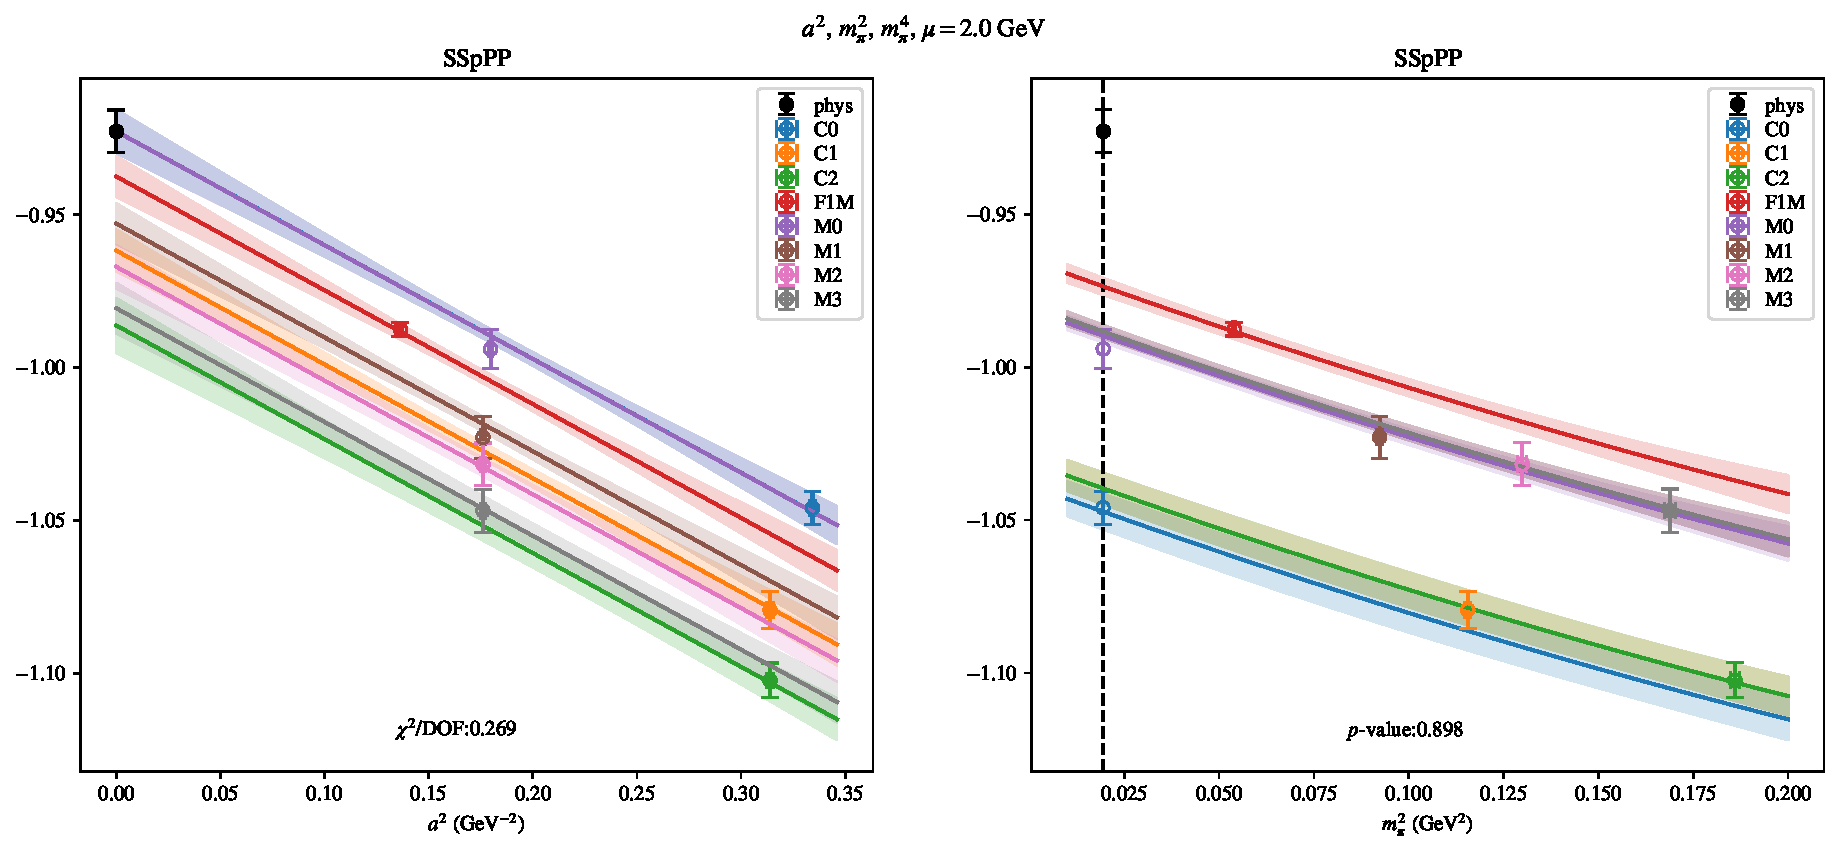
\includepdf[link, pages=-]{VVmAA/SUSY/a2m2m4_20.pdf}
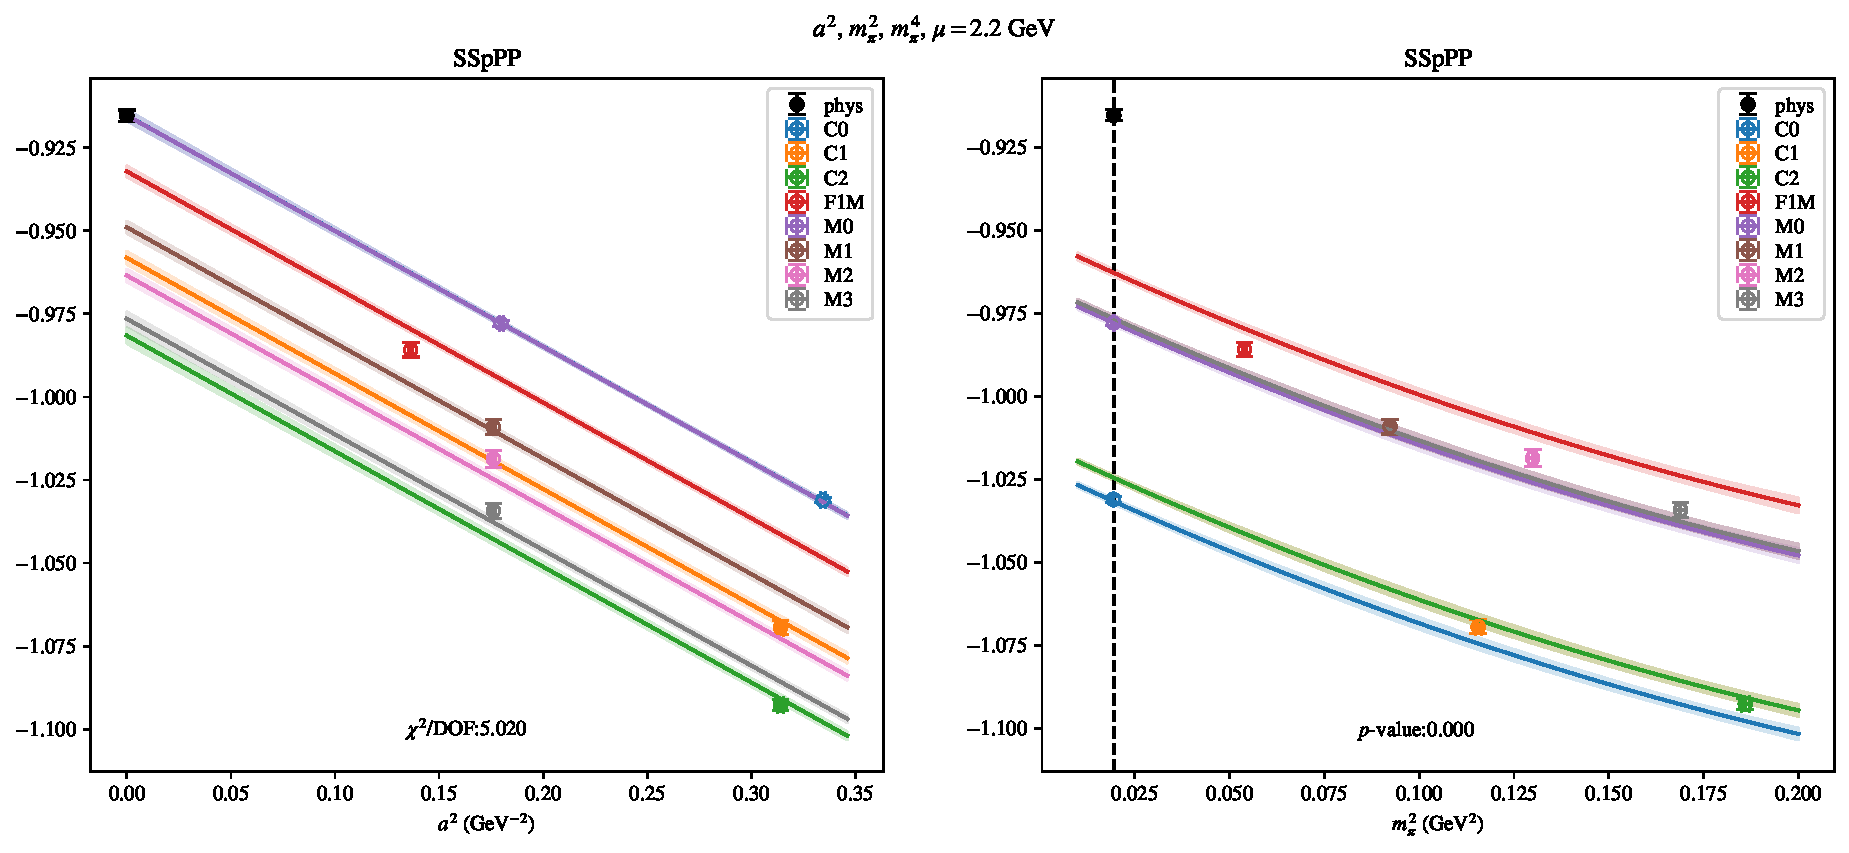
\includepdf[link, pages=-]{VVmAA/SUSY/a2m2m4_22.pdf}
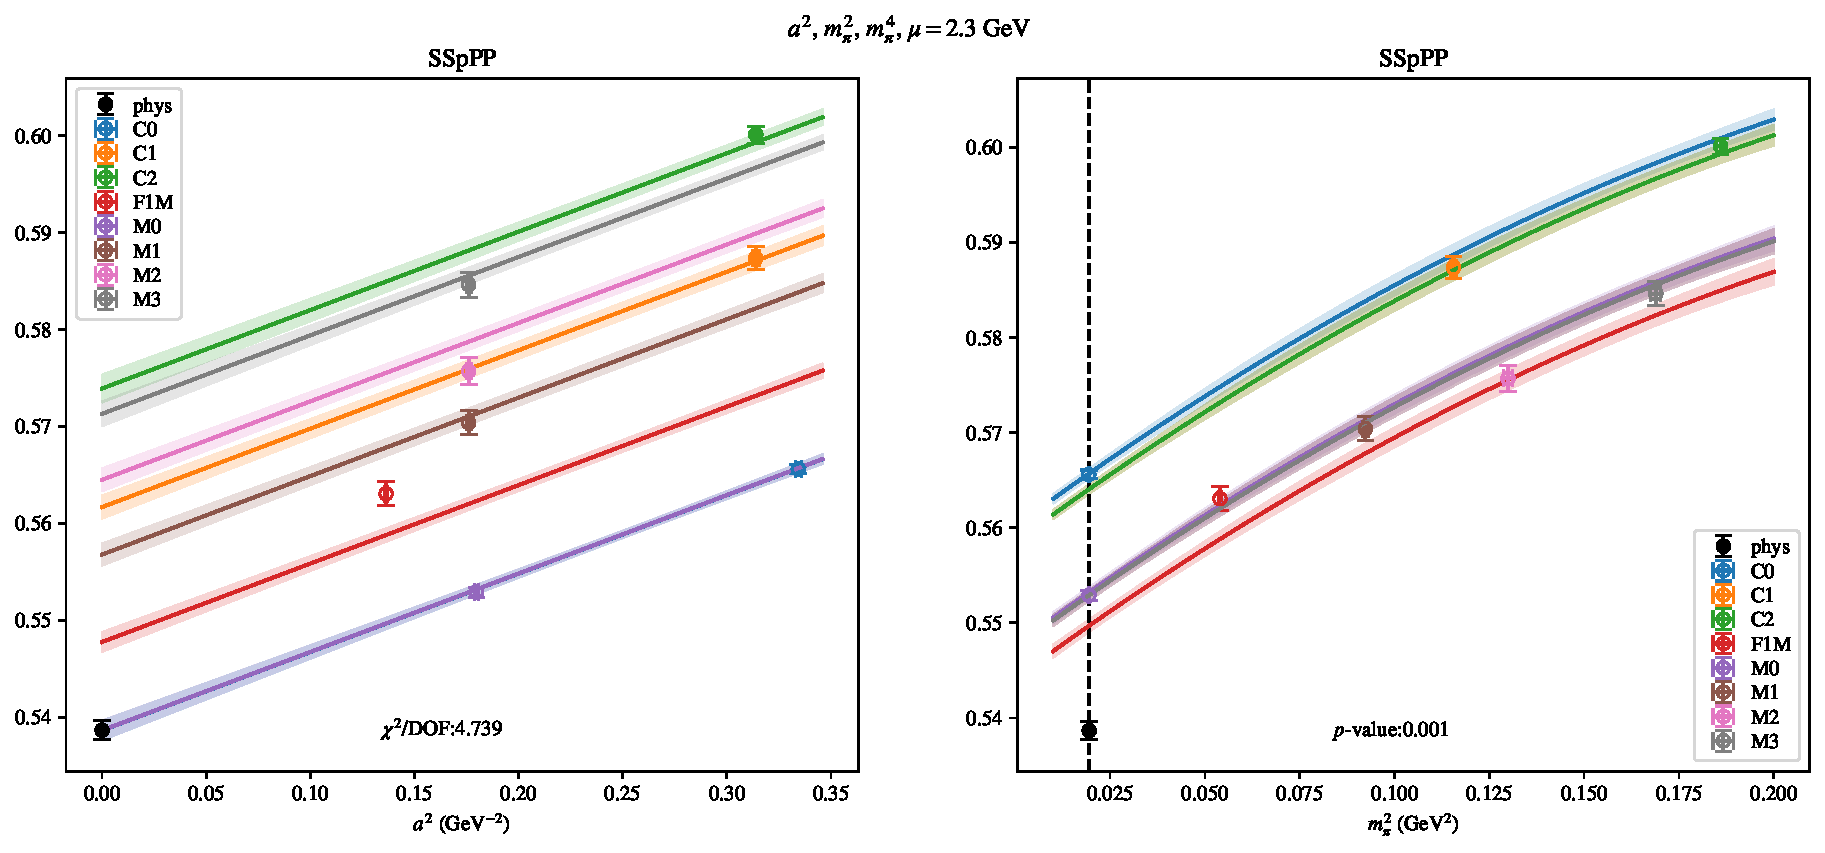
\includepdf[link, pages=-]{VVmAA/SUSY/a2m2m4_23.pdf}
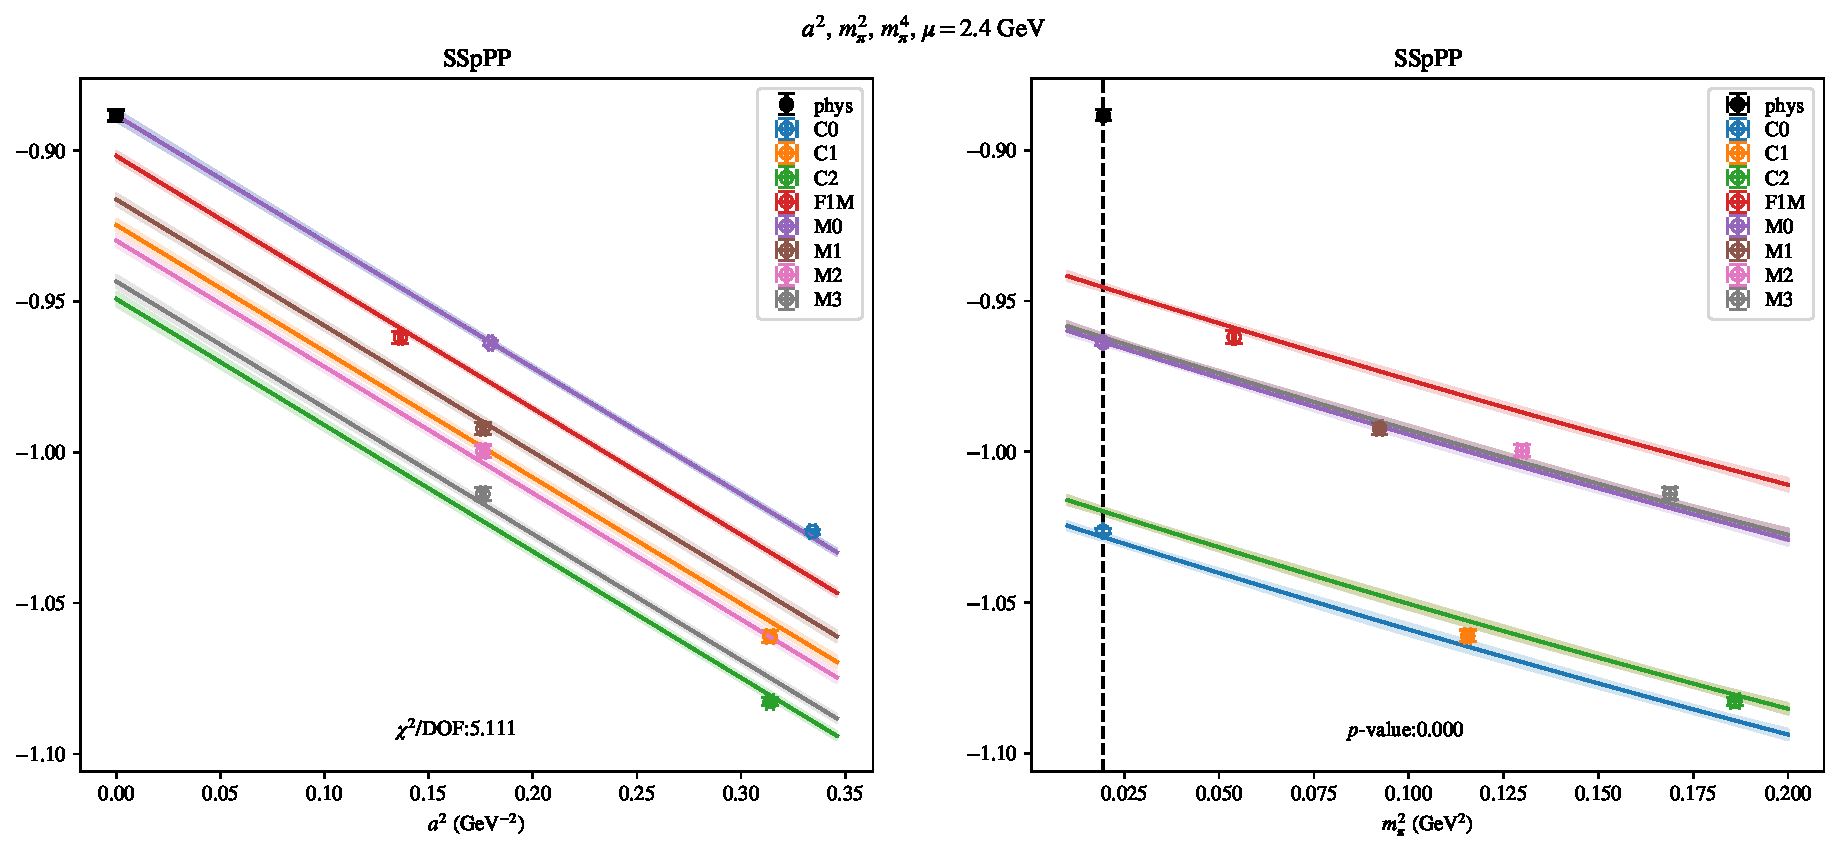
\includepdf[link, pages=-]{VVmAA/SUSY/a2m2m4_24.pdf}
\clearpage
\section{$B_3$}
\begin{table}[h!]
\begin{center}
\begin{tabular}{|c|c|c|c|c|c|}
\hline
$\mu$ (GeV) & $a^2$, $m_\pi^2$& $a^2$, $m_\pi^2$ (no C)& $a^2$, $a^4$, $m_\pi^2$& $a^2$, $m_\pi^2$ (no M3, C2)& $a^2$, $m_\pi^2$, $m_\pi^4$\\
\hline
2.0& \hyperlink{SSmPP/SUSY/a2m2_20.pdf.1}{\textbf{1.4242(59)}: 6.678 (0.0)} & \hyperlink{SSmPP/SUSY/a2m2noC_20.pdf.1}{\textbf{1.538(13)}: 1.548 (0.213)} & \hyperlink{SSmPP/SUSY/a2a4m2_20.pdf.1}{\textbf{1.617(22)}: 1.737 (0.139)} & \hyperlink{SSmPP/SUSY/a2m2mcut_20.pdf.1}{\textbf{1.4218(57)}: 10.396 (0.0)} & \hyperlink{SSmPP/SUSY/a2m2m4_20.pdf.1}{\textbf{1.4169(57)}: 6.379 (0.0)}\\
2.2& \hyperlink{SSmPP/SUSY/a2m2_22.pdf.1}{\textbf{1.2699(57)}: 6.439 (0.0)} & \hyperlink{SSmPP/SUSY/a2m2noC_22.pdf.1}{\textbf{1.384(13)}: 1.173 (0.309)} & \hyperlink{SSmPP/SUSY/a2a4m2_22.pdf.1}{\textbf{1.441(21)}: 2.431 (0.045)} & \hyperlink{SSmPP/SUSY/a2m2mcut_22.pdf.1}{\textbf{1.2684(55)}: 9.623 (0.0)} & \hyperlink{SSmPP/SUSY/a2m2m4_22.pdf.1}{\textbf{1.2640(54)}: 6.06 (0.0)}\\
2.3& \hyperlink{SSmPP/SUSY/a2m2_23.pdf.1}{\textbf{1.2061(51)}: 7.898 (0.0)} & \hyperlink{SSmPP/SUSY/a2m2noC_23.pdf.1}{\textbf{1.321(12)}: 1.016 (0.362)} & \hyperlink{SSmPP/SUSY/a2a4m2_23.pdf.1}{\textbf{1.385(20)}: 2.208 (0.065)} & \hyperlink{SSmPP/SUSY/a2m2mcut_23.pdf.1}{\textbf{1.2044(48)}: 12.011 (0.0)} & \hyperlink{SSmPP/SUSY/a2m2m4_23.pdf.1}{\textbf{1.2004(47)}: 7.491 (0.0)}\\
2.4& \hyperlink{SSmPP/SUSY/a2m2_24.pdf.1}{\textbf{1.1559(48)}: 7.08 (0.0)} & \hyperlink{SSmPP/SUSY/a2m2noC_24.pdf.1}{\textbf{1.255(11)}: 0.938 (0.391)} & \hyperlink{SSmPP/SUSY/a2a4m2_24.pdf.1}{\textbf{1.303(18)}: 2.848 (0.022)} & \hyperlink{SSmPP/SUSY/a2m2mcut_24.pdf.1}{\textbf{1.1547(47)}: 10.751 (0.0)} & \hyperlink{SSmPP/SUSY/a2m2m4_24.pdf.1}{\textbf{1.1503(46)}: 6.884 (0.0)}\\
\hline
\end{tabular}
\caption{Physical point value from chiral and continuum extrapolation at renormalisation scale $\mu$. Entries are \textbf{value(error)}: $\chi^2/\text{DOF}$ ($p$-value).}
\end{center}
\end{table}
\begin{table}[h!]
\begin{center}
\begin{tabular}{|c c|c|c|c|c|c|}
\hline
$\mu$ (GeV) &  & $a^2$, $m_\pi^2$& $a^2$, $m_\pi^2$ (no C)& $a^2$, $a^4$, $m_\pi^2$& $a^2$, $m_\pi^2$ (no M3, C2)& $a^2$, $m_\pi^2$, $m_\pi^4$\\
\hline
\multirow{2}{0.5in}{2.0} & $\alpha$ & -0.532(54)& -0.94(42)& -1.5(10)& -0.529(57)& -0.521(55)\\
 & $\beta$ & 0.00669(17)& 0.00674(27)& 0.00651(15)& 0.00725(27)& 0.01042(64)\\
\hline
\multirow{2}{0.5in}{2.2} & $\alpha$ & -0.476(64)& -0.92(42)& -1.5(10)& -0.475(65)& -0.466(63)\\
 & $\beta$ & 0.00657(14)& 0.00622(23)& 0.00637(12)& 0.00720(26)& 0.01013(68)\\
\hline
\multirow{2}{0.5in}{2.3} & $\alpha$ & -0.445(65)& -0.92(42)& -1.56(99)& -0.443(64)& -0.434(63)\\
 & $\beta$ & 0.00653(18)& 0.00622(27)& 0.00630(15)& 0.00718(30)& 0.01045(74)\\
\hline
\multirow{2}{0.5in}{2.4} & $\alpha$ & -0.428(67)& -0.86(42)& -1.4(10)& -0.427(69)& -0.417(67)\\
 & $\beta$ & 0.00657(14)& 0.00619(21)& 0.00642(12)& 0.00711(24)& 0.00989(65)\\
\hline
\end{tabular}
\caption{Fit values of coefficients in $B = B_{phys} + \mathbf{\alpha} a^2 + \mathbf{\beta}\left(\frac{m_\pi^2}{f_\pi^2}-\frac{m_{\pi,PDG}^2}{f_\pi^2}\right) + \ldots$.}
\end{center}
\end{table}
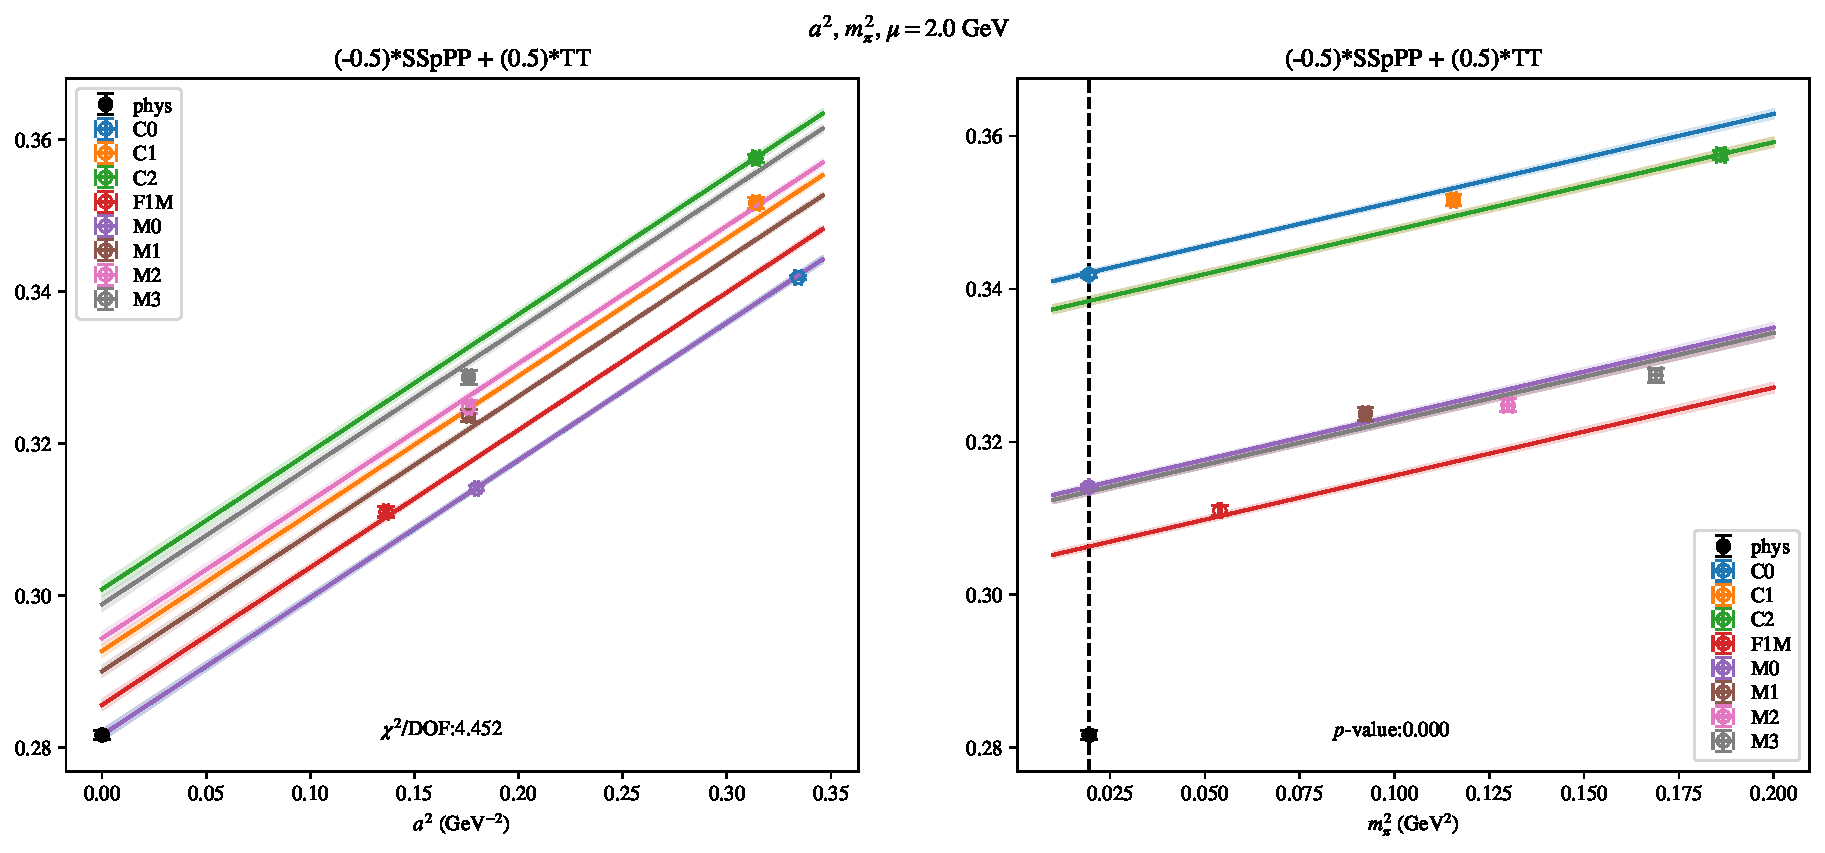
\includepdf[link, pages=-]{SSmPP/SUSY/a2m2_20.pdf}
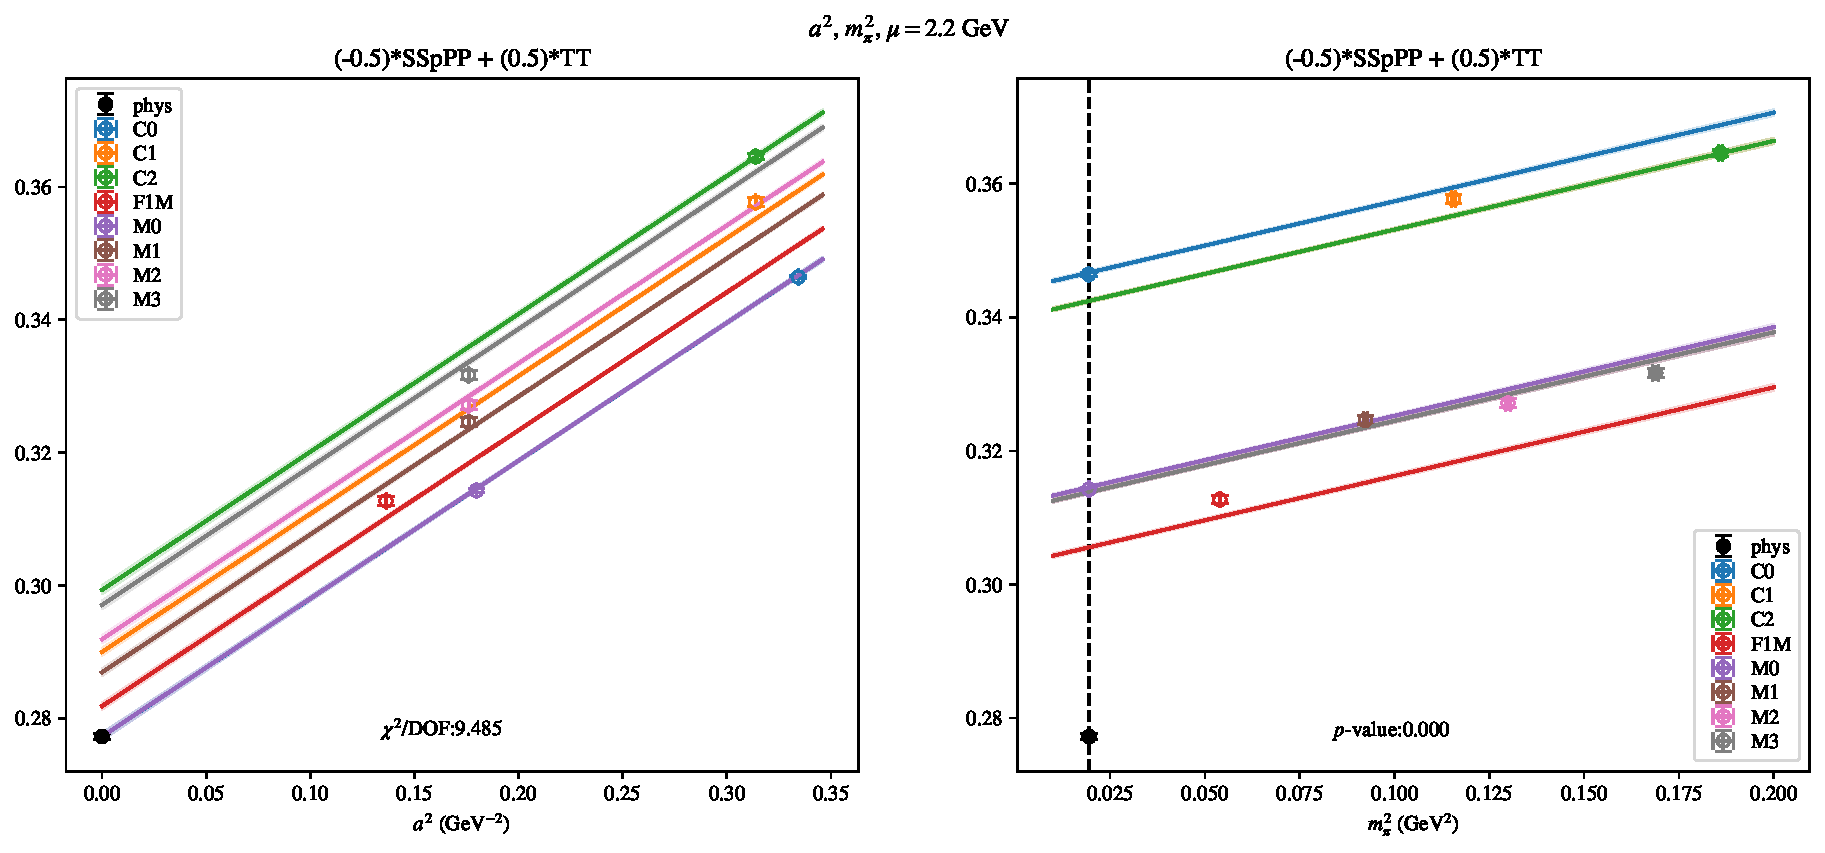
\includepdf[link, pages=-]{SSmPP/SUSY/a2m2_22.pdf}
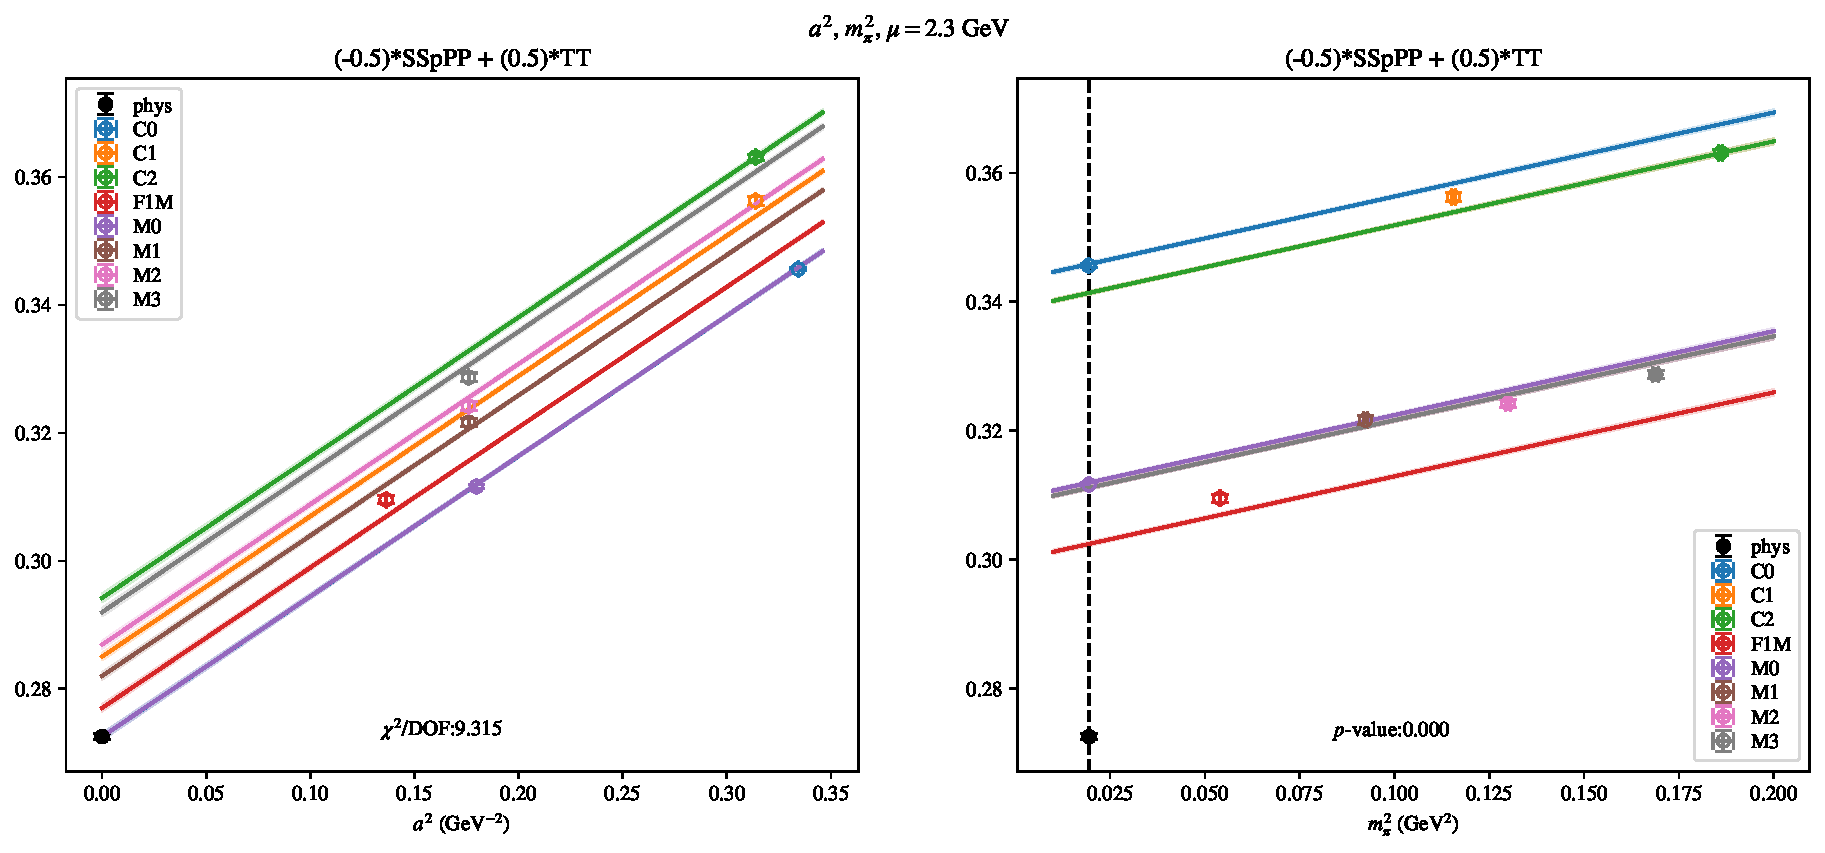
\includepdf[link, pages=-]{SSmPP/SUSY/a2m2_23.pdf}
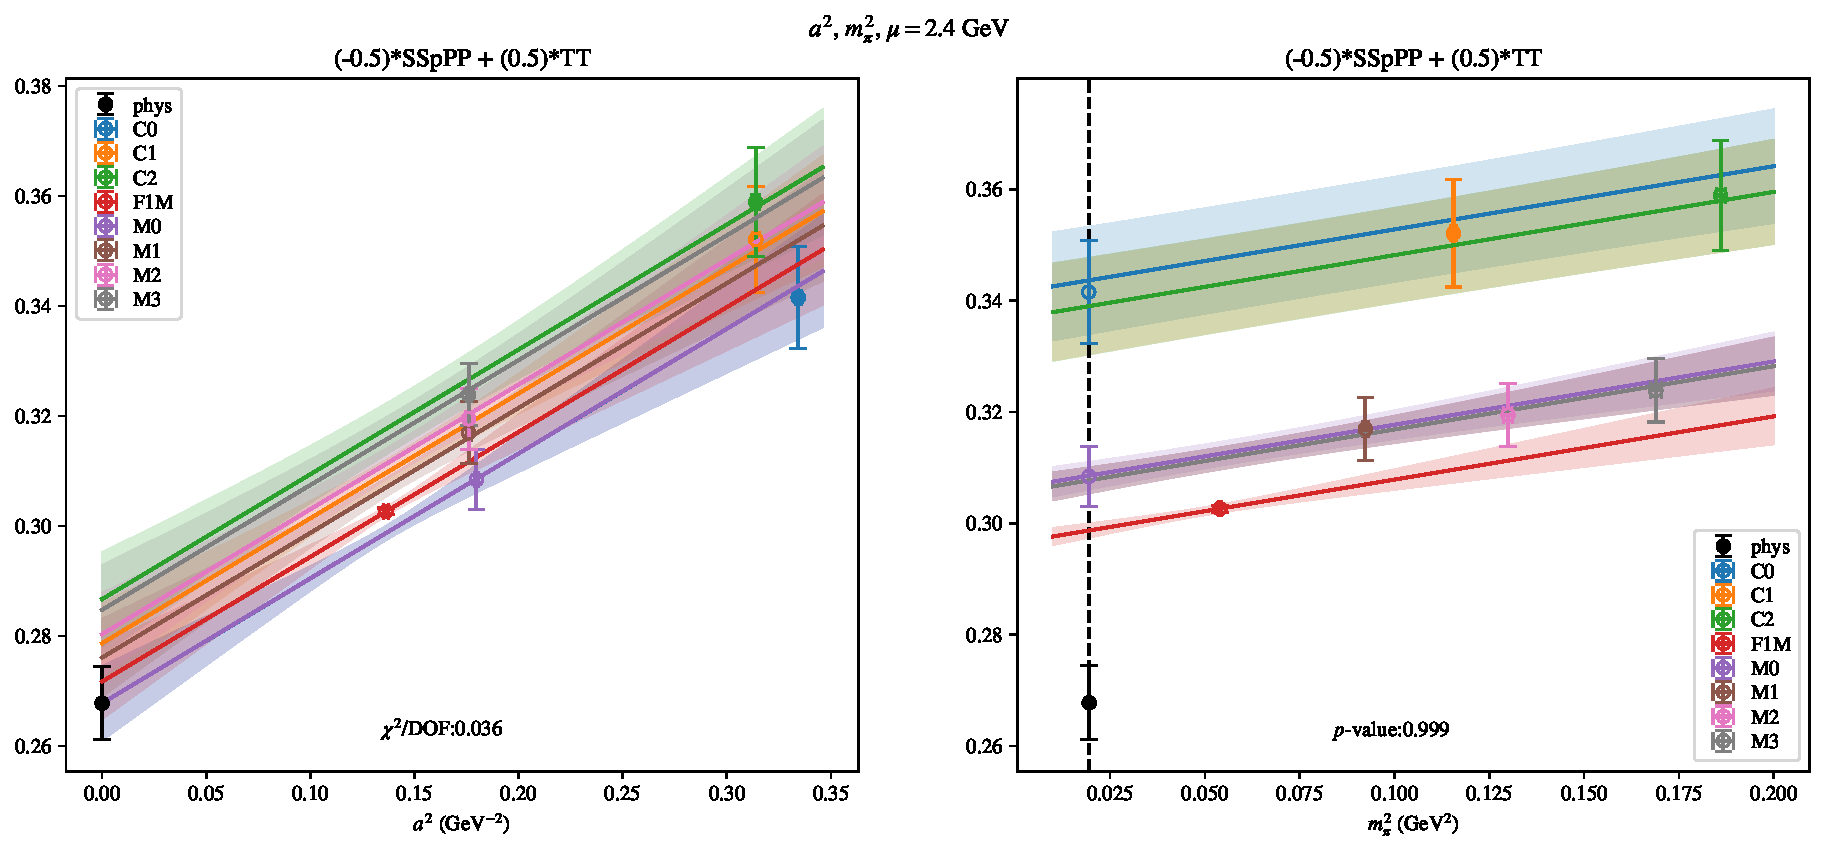
\includepdf[link, pages=-]{SSmPP/SUSY/a2m2_24.pdf}
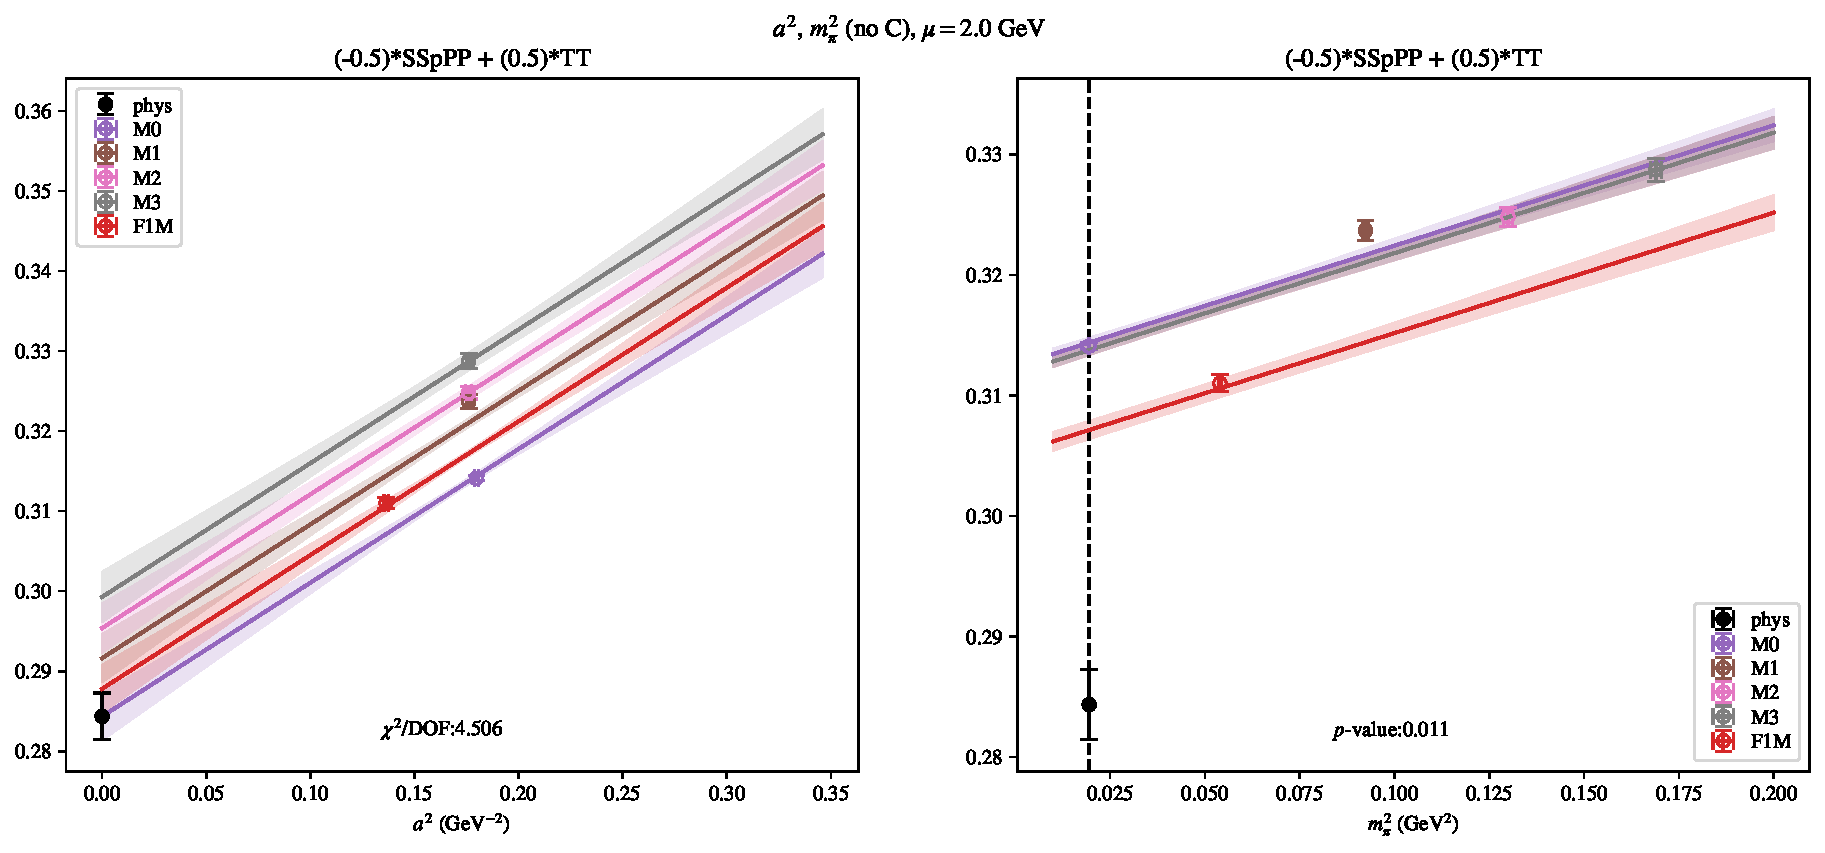
\includepdf[link, pages=-]{SSmPP/SUSY/a2m2noC_20.pdf}
\includepdf[link, pages=-]{SSmPP/SUSY/a2m2noC_22.pdf}
\includepdf[link, pages=-]{SSmPP/SUSY/a2m2noC_23.pdf}
\includepdf[link, pages=-]{SSmPP/SUSY/a2m2noC_24.pdf}
\includepdf[link, pages=-]{SSmPP/SUSY/a2a4m2_20.pdf}
\includepdf[link, pages=-]{SSmPP/SUSY/a2a4m2_22.pdf}
\includepdf[link, pages=-]{SSmPP/SUSY/a2a4m2_23.pdf}
\includepdf[link, pages=-]{SSmPP/SUSY/a2a4m2_24.pdf}
\includepdf[link, pages=-]{SSmPP/SUSY/a2m2mcut_20.pdf}
\includepdf[link, pages=-]{SSmPP/SUSY/a2m2mcut_22.pdf}
\includepdf[link, pages=-]{SSmPP/SUSY/a2m2mcut_23.pdf}
\includepdf[link, pages=-]{SSmPP/SUSY/a2m2mcut_24.pdf}
\includepdf[link, pages=-]{SSmPP/SUSY/a2m2m4_20.pdf}
\includepdf[link, pages=-]{SSmPP/SUSY/a2m2m4_22.pdf}
\includepdf[link, pages=-]{SSmPP/SUSY/a2m2m4_23.pdf}
\includepdf[link, pages=-]{SSmPP/SUSY/a2m2m4_24.pdf}
\clearpage
\section{$B_4$}
\begin{table}[h!]
\begin{center}
\begin{tabular}{|c|c|c|c|c|c|}
\hline
$\mu$ (GeV) & $a^2$, $m_\pi^2$& $a^2$, $m_\pi^2$ (no C)& $a^2$, $a^4$, $m_\pi^2$& $a^2$, $m_\pi^2$ (no M3, C2)& $a^2$, $m_\pi^2$, $m_\pi^4$\\
\hline
2.0& \hyperlink{SSpPP/SUSY/a2m2_20.pdf.1}{\textbf{0.8933(12)}: 5.868 (0.0)} & \hyperlink{SSpPP/SUSY/a2m2noC_20.pdf.1}{\textbf{0.8650(63)}: 3.742 (0.024)} & \hyperlink{SSpPP/SUSY/a2a4m2_20.pdf.1}{\textbf{0.8487(99)}: 2.386 (0.049)} & \hyperlink{SSpPP/SUSY/a2m2mcut_20.pdf.1}{\textbf{0.8936(14)}: 8.105 (0.0)} & \hyperlink{SSpPP/SUSY/a2m2m4_20.pdf.1}{\textbf{0.8952(13)}: 4.901 (0.001)}\\
2.2& \hyperlink{SSpPP/SUSY/a2m2_22.pdf.1}{\textbf{0.8914(12)}: 5.589 (0.0)} & \hyperlink{SSpPP/SUSY/a2m2noC_22.pdf.1}{\textbf{0.8625(61)}: 2.292 (0.101)} & \hyperlink{SSpPP/SUSY/a2a4m2_22.pdf.1}{\textbf{0.8455(97)}: 1.6 (0.171)} & \hyperlink{SSpPP/SUSY/a2m2mcut_22.pdf.1}{\textbf{0.8916(13)}: 8.056 (0.0)} & \hyperlink{SSpPP/SUSY/a2m2m4_22.pdf.1}{\textbf{0.8930(13)}: 5.111 (0.0)}\\
2.3& \hyperlink{SSpPP/SUSY/a2m2_23.pdf.1}{\textbf{0.8907(12)}: 5.937 (0.0)} & \hyperlink{SSpPP/SUSY/a2m2noC_23.pdf.1}{\textbf{0.8609(61)}: 2.329 (0.097)} & \hyperlink{SSpPP/SUSY/a2a4m2_23.pdf.1}{\textbf{0.8437(97)}: 1.748 (0.136)} & \hyperlink{SSpPP/SUSY/a2m2mcut_23.pdf.1}{\textbf{0.8910(13)}: 8.55 (0.0)} & \hyperlink{SSpPP/SUSY/a2m2m4_23.pdf.1}{\textbf{0.8925(13)}: 5.346 (0.0)}\\
2.4& \hyperlink{SSpPP/SUSY/a2m2_24.pdf.1}{\textbf{0.8903(12)}: 6.602 (0.0)} & \hyperlink{SSpPP/SUSY/a2m2noC_24.pdf.1}{\textbf{0.8592(60)}: 2.687 (0.068)} & \hyperlink{SSpPP/SUSY/a2a4m2_24.pdf.1}{\textbf{0.8411(96)}: 1.962 (0.097)} & \hyperlink{SSpPP/SUSY/a2m2mcut_24.pdf.1}{\textbf{0.8906(13)}: 9.521 (0.0)} & \hyperlink{SSpPP/SUSY/a2m2m4_24.pdf.1}{\textbf{0.8922(13)}: 5.918 (0.0)}\\
\hline
\end{tabular}
\caption{Physical point value from chiral and continuum extrapolation at renormalisation scale $\mu$. Entries are \textbf{value(error)}: $\chi^2/\text{DOF}$ ($p$-value).}
\end{center}
\end{table}
\begin{table}[h!]
\begin{center}
\begin{tabular}{|c c|c|c|c|c|c|}
\hline
$\mu$ (GeV) &  & $a^2$, $m_\pi^2$& $a^2$, $m_\pi^2$ (no C)& $a^2$, $a^4$, $m_\pi^2$& $a^2$, $m_\pi^2$ (no M3, C2)& $a^2$, $m_\pi^2$, $m_\pi^4$\\
\hline
\multirow{2}{0.5in}{2.0} & $\alpha$ & 0.0113(53)& 0.201(42)& 0.48(11)& 0.0106(59)& 0.0043(58)\\
 & $\beta$ & -0.0& -0.0& -0.0002(14)& -0.0003(23)& -0.0020(63)\\
\hline
\multirow{2}{0.5in}{2.2} & $\alpha$ & 0.0015(51)& 0.196(41)& 0.48(10)& 0.0011(56)& -0.004(57)\\
 & $\beta$ & -0.0003(12)& -0.0003(22)& -0.0005(13)& -0.0006(23)& -0.0020(66)\\
\hline
\multirow{2}{0.5in}{2.3} & $\alpha$ & -0.002(51)& 0.198(41)& 0.49(10)& -0.003(56)& -0.009(56)\\
 & $\beta$ & -0.0004(11)& -0.0003(20)& -0.0006(13)& -0.0007(21)& -0.0021(63)\\
\hline
\multirow{2}{0.5in}{2.4} & $\alpha$ & -0.006(51)& 0.203(41)& 0.51(10)& -0.007(56)& -0.013(56)\\
 & $\beta$ & -0.0004(11)& -0.0004(20)& -0.0006(12)& -0.0007(20)& -0.0023(61)\\
\hline
\end{tabular}
\caption{Fit values of coefficients in $B = B_{phys} + \mathbf{\alpha} a^2 + \mathbf{\beta}\left(\frac{m_\pi^2}{f_\pi^2}-\frac{m_{\pi,PDG}^2}{f_\pi^2}\right) + \ldots$.}
\end{center}
\end{table}
\includepdf[link, pages=-]{SSpPP/SUSY/a2m2_20.pdf}
\includepdf[link, pages=-]{SSpPP/SUSY/a2m2_22.pdf}
\includepdf[link, pages=-]{SSpPP/SUSY/a2m2_23.pdf}
\includepdf[link, pages=-]{SSpPP/SUSY/a2m2_24.pdf}
\includepdf[link, pages=-]{SSpPP/SUSY/a2m2noC_20.pdf}
\includepdf[link, pages=-]{SSpPP/SUSY/a2m2noC_22.pdf}
\includepdf[link, pages=-]{SSpPP/SUSY/a2m2noC_23.pdf}
\includepdf[link, pages=-]{SSpPP/SUSY/a2m2noC_24.pdf}
\includepdf[link, pages=-]{SSpPP/SUSY/a2a4m2_20.pdf}
\includepdf[link, pages=-]{SSpPP/SUSY/a2a4m2_22.pdf}
\includepdf[link, pages=-]{SSpPP/SUSY/a2a4m2_23.pdf}
\includepdf[link, pages=-]{SSpPP/SUSY/a2a4m2_24.pdf}
\includepdf[link, pages=-]{SSpPP/SUSY/a2m2mcut_20.pdf}
\includepdf[link, pages=-]{SSpPP/SUSY/a2m2mcut_22.pdf}
\includepdf[link, pages=-]{SSpPP/SUSY/a2m2mcut_23.pdf}
\includepdf[link, pages=-]{SSpPP/SUSY/a2m2mcut_24.pdf}
\includepdf[link, pages=-]{SSpPP/SUSY/a2m2m4_20.pdf}
\includepdf[link, pages=-]{SSpPP/SUSY/a2m2m4_22.pdf}
\includepdf[link, pages=-]{SSpPP/SUSY/a2m2m4_23.pdf}
\includepdf[link, pages=-]{SSpPP/SUSY/a2m2m4_24.pdf}
\clearpage
\section{$B_5$}
\begin{table}[h!]
\begin{center}
\begin{tabular}{|c|c|c|c|c|c|}
\hline
$\mu$ (GeV) & $a^2$, $m_\pi^2$& $a^2$, $m_\pi^2$ (no C)& $a^2$, $a^4$, $m_\pi^2$& $a^2$, $m_\pi^2$ (no M3, C2)& $a^2$, $m_\pi^2$, $m_\pi^4$\\
\hline
2.0& \hyperlink{TT/SUSY/a2m2_20.pdf.1}{\textbf{1.4071(37)}: 1.075 (0.372)} & \hyperlink{TT/SUSY/a2m2noC_20.pdf.1}{\textbf{1.429(10)}: 0.442 (0.643)} & \hyperlink{TT/SUSY/a2a4m2_20.pdf.1}{\textbf{1.455(16)}: 0.346 (0.847)} & \hyperlink{TT/SUSY/a2m2mcut_20.pdf.1}{\textbf{1.4063(34)}: 1.389 (0.244)} & \hyperlink{TT/SUSY/a2m2m4_20.pdf.1}{\textbf{1.4069(34)}: 1.341 (0.252)}\\
2.2& \hyperlink{TT/SUSY/a2m2_22.pdf.1}{\textbf{1.3216(37)}: 0.812 (0.541)} & \hyperlink{TT/SUSY/a2m2noC_22.pdf.1}{\textbf{1.346(10)}: 0.387 (0.679)} & \hyperlink{TT/SUSY/a2a4m2_22.pdf.1}{\textbf{1.364(16)}: 0.204 (0.936)} & \hyperlink{TT/SUSY/a2m2mcut_22.pdf.1}{\textbf{1.3211(34)}: 1.233 (0.296)} & \hyperlink{TT/SUSY/a2m2m4_22.pdf.1}{\textbf{1.3214(34)}: 1.01 (0.401)}\\
2.3& \hyperlink{TT/SUSY/a2m2_23.pdf.1}{\textbf{1.2852(33)}: 1.099 (0.358)} & \hyperlink{TT/SUSY/a2m2noC_23.pdf.1}{\textbf{1.310(10)}: 0.477 (0.62)} & \hyperlink{TT/SUSY/a2a4m2_23.pdf.1}{\textbf{1.332(15)}: 0.246 (0.912)} & \hyperlink{TT/SUSY/a2m2mcut_23.pdf.1}{\textbf{1.2847(31)}: 1.649 (0.176)} & \hyperlink{TT/SUSY/a2m2m4_23.pdf.1}{\textbf{1.2849(30)}: 1.363 (0.244)}\\
2.4& \hyperlink{TT/SUSY/a2m2_24.pdf.1}{\textbf{1.2556(32)}: 0.88 (0.494)} & \hyperlink{TT/SUSY/a2m2noC_24.pdf.1}{\textbf{1.2744(97)}: 0.94 (0.391)} & \hyperlink{TT/SUSY/a2a4m2_24.pdf.1}{\textbf{1.288(14)}: 0.474 (0.755)} & \hyperlink{TT/SUSY/a2m2mcut_24.pdf.1}{\textbf{1.2553(30)}: 1.247 (0.291)} & \hyperlink{TT/SUSY/a2m2m4_24.pdf.1}{\textbf{1.2559(30)}: 1.09 (0.36)}\\
\hline
\end{tabular}
\caption{Physical point value from chiral and continuum extrapolation at renormalisation scale $\mu$. Entries are \textbf{value(error)}: $\chi^2/\text{DOF}$ ($p$-value).}
\end{center}
\end{table}
\begin{table}[h!]
\begin{center}
\begin{tabular}{|c c|c|c|c|c|c|}
\hline
$\mu$ (GeV) &  & $a^2$, $m_\pi^2$& $a^2$, $m_\pi^2$ (no C)& $a^2$, $a^4$, $m_\pi^2$& $a^2$, $m_\pi^2$ (no M3, C2)& $a^2$, $m_\pi^2$, $m_\pi^4$\\
\hline
\multirow{2}{0.5in}{2.0} & $\alpha$ & -0.523(42)& -0.61(37)& -0.80(91)& -0.521(45)& -0.522(44)\\
 & $\beta$ & 0.00146(15)& 0.00177(25)& 0.00156(14)& 0.00140(25)& 0.00156(64)\\
\hline
\multirow{2}{0.5in}{2.2} & $\alpha$ & -0.493(45)& -0.59(37)& -0.76(92)& -0.491(45)& -0.492(45)\\
 & $\beta$ & 0.00117(12)& 0.00129(22)& 0.00128(12)& 0.00114(25)& 0.00130(68)\\
\hline
\multirow{2}{0.5in}{2.3} & $\alpha$ & -0.475(44)& -0.58(37)& -0.77(91)& -0.474(44)& -0.475(44)\\
 & $\beta$ & 0.00108(13)& 0.00123(23)& 0.00119(13)& 0.00105(25)& 0.00126(68)\\
\hline
\multirow{2}{0.5in}{2.4} & $\alpha$ & -0.465(45)& -0.54(37)& -0.68(92)& -0.464(46)& -0.466(46)\\
 & $\beta$ & 0.00109(11)& 0.00117(20)& 0.00118(11)& 0.00100(22)& 0.00093(63)\\
\hline
\end{tabular}
\caption{Fit values of coefficients in $B = B_{phys} + \mathbf{\alpha} a^2 + \mathbf{\beta}\left(\frac{m_\pi^2}{f_\pi^2}-\frac{m_{\pi,PDG}^2}{f_\pi^2}\right) + \ldots$.}
\end{center}
\end{table}
\includepdf[link, pages=-]{TT/SUSY/a2m2_20.pdf}
\includepdf[link, pages=-]{TT/SUSY/a2m2_22.pdf}
\includepdf[link, pages=-]{TT/SUSY/a2m2_23.pdf}
\includepdf[link, pages=-]{TT/SUSY/a2m2_24.pdf}
\includepdf[link, pages=-]{TT/SUSY/a2m2noC_20.pdf}
\includepdf[link, pages=-]{TT/SUSY/a2m2noC_22.pdf}
\includepdf[link, pages=-]{TT/SUSY/a2m2noC_23.pdf}
\includepdf[link, pages=-]{TT/SUSY/a2m2noC_24.pdf}
\includepdf[link, pages=-]{TT/SUSY/a2a4m2_20.pdf}
\includepdf[link, pages=-]{TT/SUSY/a2a4m2_22.pdf}
\includepdf[link, pages=-]{TT/SUSY/a2a4m2_23.pdf}
\includepdf[link, pages=-]{TT/SUSY/a2a4m2_24.pdf}
\includepdf[link, pages=-]{TT/SUSY/a2m2mcut_20.pdf}
\includepdf[link, pages=-]{TT/SUSY/a2m2mcut_22.pdf}
\includepdf[link, pages=-]{TT/SUSY/a2m2mcut_23.pdf}
\includepdf[link, pages=-]{TT/SUSY/a2m2mcut_24.pdf}
\includepdf[link, pages=-]{TT/SUSY/a2m2m4_20.pdf}
\includepdf[link, pages=-]{TT/SUSY/a2m2m4_22.pdf}
\includepdf[link, pages=-]{TT/SUSY/a2m2m4_23.pdf}
\includepdf[link, pages=-]{TT/SUSY/a2m2m4_24.pdf}
\clearpage
\end{document}